As we mentioned at the begining of chapter 4, The analysis is designed for maximum sensitivity to the SUSY simplified model T2tt, T1tttt, T1ttbb, T5tttt and T5ttcc topology (see Fig~\ref{Fig:signal_diagrams}) resulting in final states with multiple top quarks, hence multiple jets and b-tagged jets, produced in stop decay, no leptons, and large \MET. The T2tt, T5ttcc and T1tttt final states differ in the number of jets, b-tagged jets and top quarks produced. 

Targeting the above-mentioned final states, data are initially selected 
by requiring a number of jets and b-jets (\njets and \nbjets) and a large \MET. 
The search regions are ultimately defined in exclusive bins of 
\ntops, \nbjets, \HT, \MET and \MTTwo, with \MTTwo to be defined in 
Sec.~\ref{sec:searchregions}. SM backgrounds come from processes such as QCD
multijet events, Z+jets, W/top+jets, and smaller contributions from rare
processes.

The data selection process starts with the triggers and follows with a 
pre-selection and the definition of the search bins. The top reconstruction
and identification procedure (top tagging) is described in this section, 
as well as the Monte Carlo (MC) samples that model signal and backgrounds.

\subsection{Trigger}
\label{sec:trig}
Six search triggers are used to collect events for this analysis. They are
seeded by \MET seed in Level-1 trigger. 
\begin{itemize}
\item \texttt{ HLT\_PFMET100\_PFMHT100\_IDTight\_v*}
\item \texttt{ HLT\_PFMET110\_PFMHT110\_IDTight\_v*}
\item \texttt{ HLT\_PFMET120\_PFMHT120\_IDTight\_v*}
\item \texttt{ HLT\_PFMETNoMu100\_PFMHTNoMu100\_IDTight\_v*} 
\item \texttt{ HLT\_PFMETNoMu110\_PFMHTNoMu110\_IDTight\_v* }
\item \texttt{ HLT\_PFMETNoMu120\_PFMHTNoMu120\_IDTight\_v*}
\end{itemize}

The probability for these triggers to accept events (trigger efficiency) is
measured in a sample of events collected by the single-electron trigger
\begin{itemize}
  \item \texttt{HLT\_Ele27\_WPTight\_v*},
\end{itemize}
which has been commonly used within CMS for the \MET trigger efficiency measurement. 
Event from the single electron dataset is required to have
\texttt{HLT\_Ele27\_WPTright\_v*} trigger, also has at least one offline
reconstructed electron with $p_{T}>$ 30GeV. These selections ensure the single
electron trigger is efficient. 

To measure the search trigger efficiency, additional cuts to mimic the
pre-selection, defined in Sec.~\ref{sec:pre-selection}, are required.
\begin{itemize}
  \item Pass all filters
  \item Veto reconstructed muon
  \item $\njets\geq4$
  \item \nbjets $\ge$ 1
  \item \HT $\ge$ 300 GeV
  \item $\Delta\phi(\MET, j_{1,2,3})>$ 0.5, 0.5, 0.3
\end{itemize}

The trigger efficiency of the search triggers is measured as a function of
the offline \MET.  The events passed the above requirements are defined as the
denominator, while the above events also triggered the search triggers are
defined as the numerator. It has been found that the \MET trigger efficiency
has a non-trivial dependency on the offline $\HT$. The search trigger
efficiencies are measured in the low $\HT$ (300 $< \HT <$ 1000) and high
$\HT$ ($\HT >$ 1000) region, as shown in Fig.~\ref{fig:TrigMET}.
\begin{figure}[tbp]
 \begin{center}
   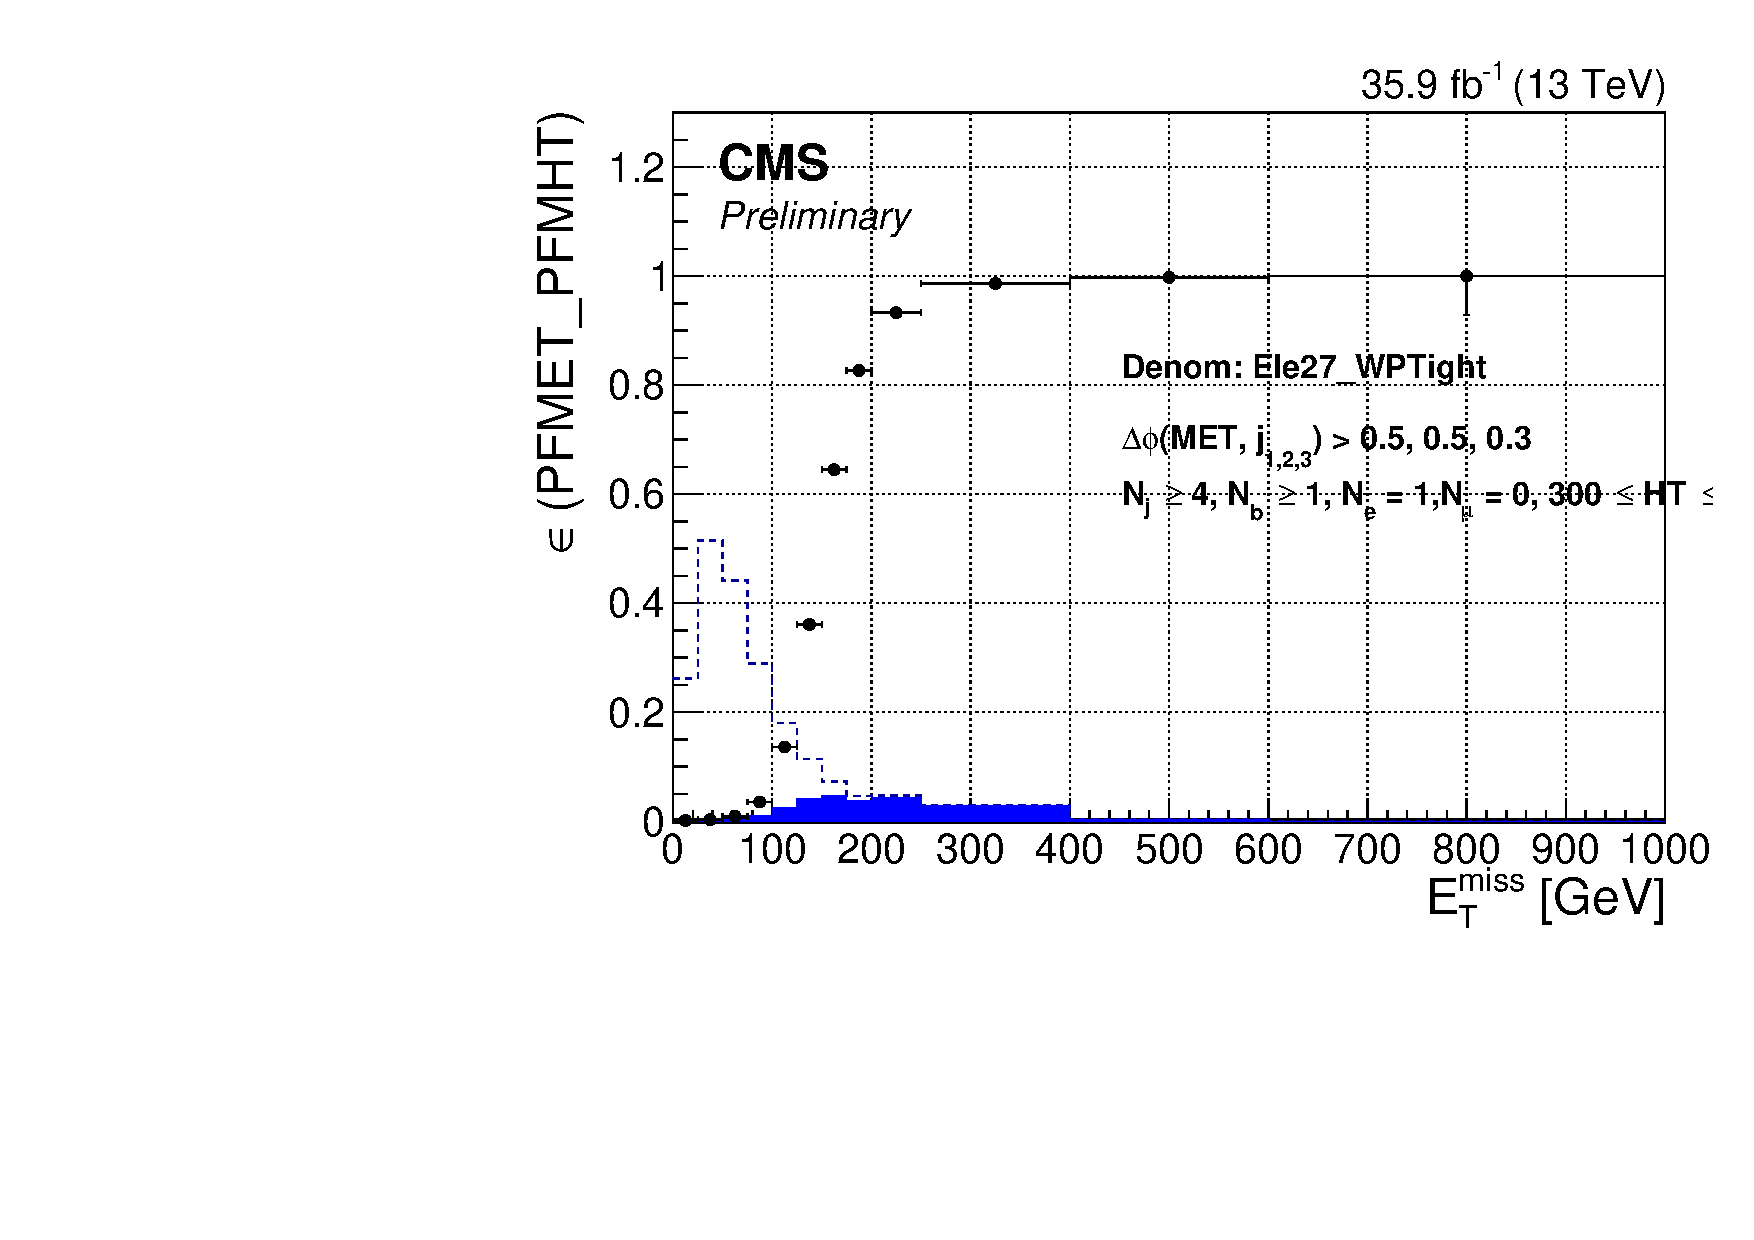
\includegraphics[width=0.49\linewidth]{sections/mc4/EvtSelSBOpt/figures/TrigEle_Stop_TrigMET_HTLess1000_9.pdf}
   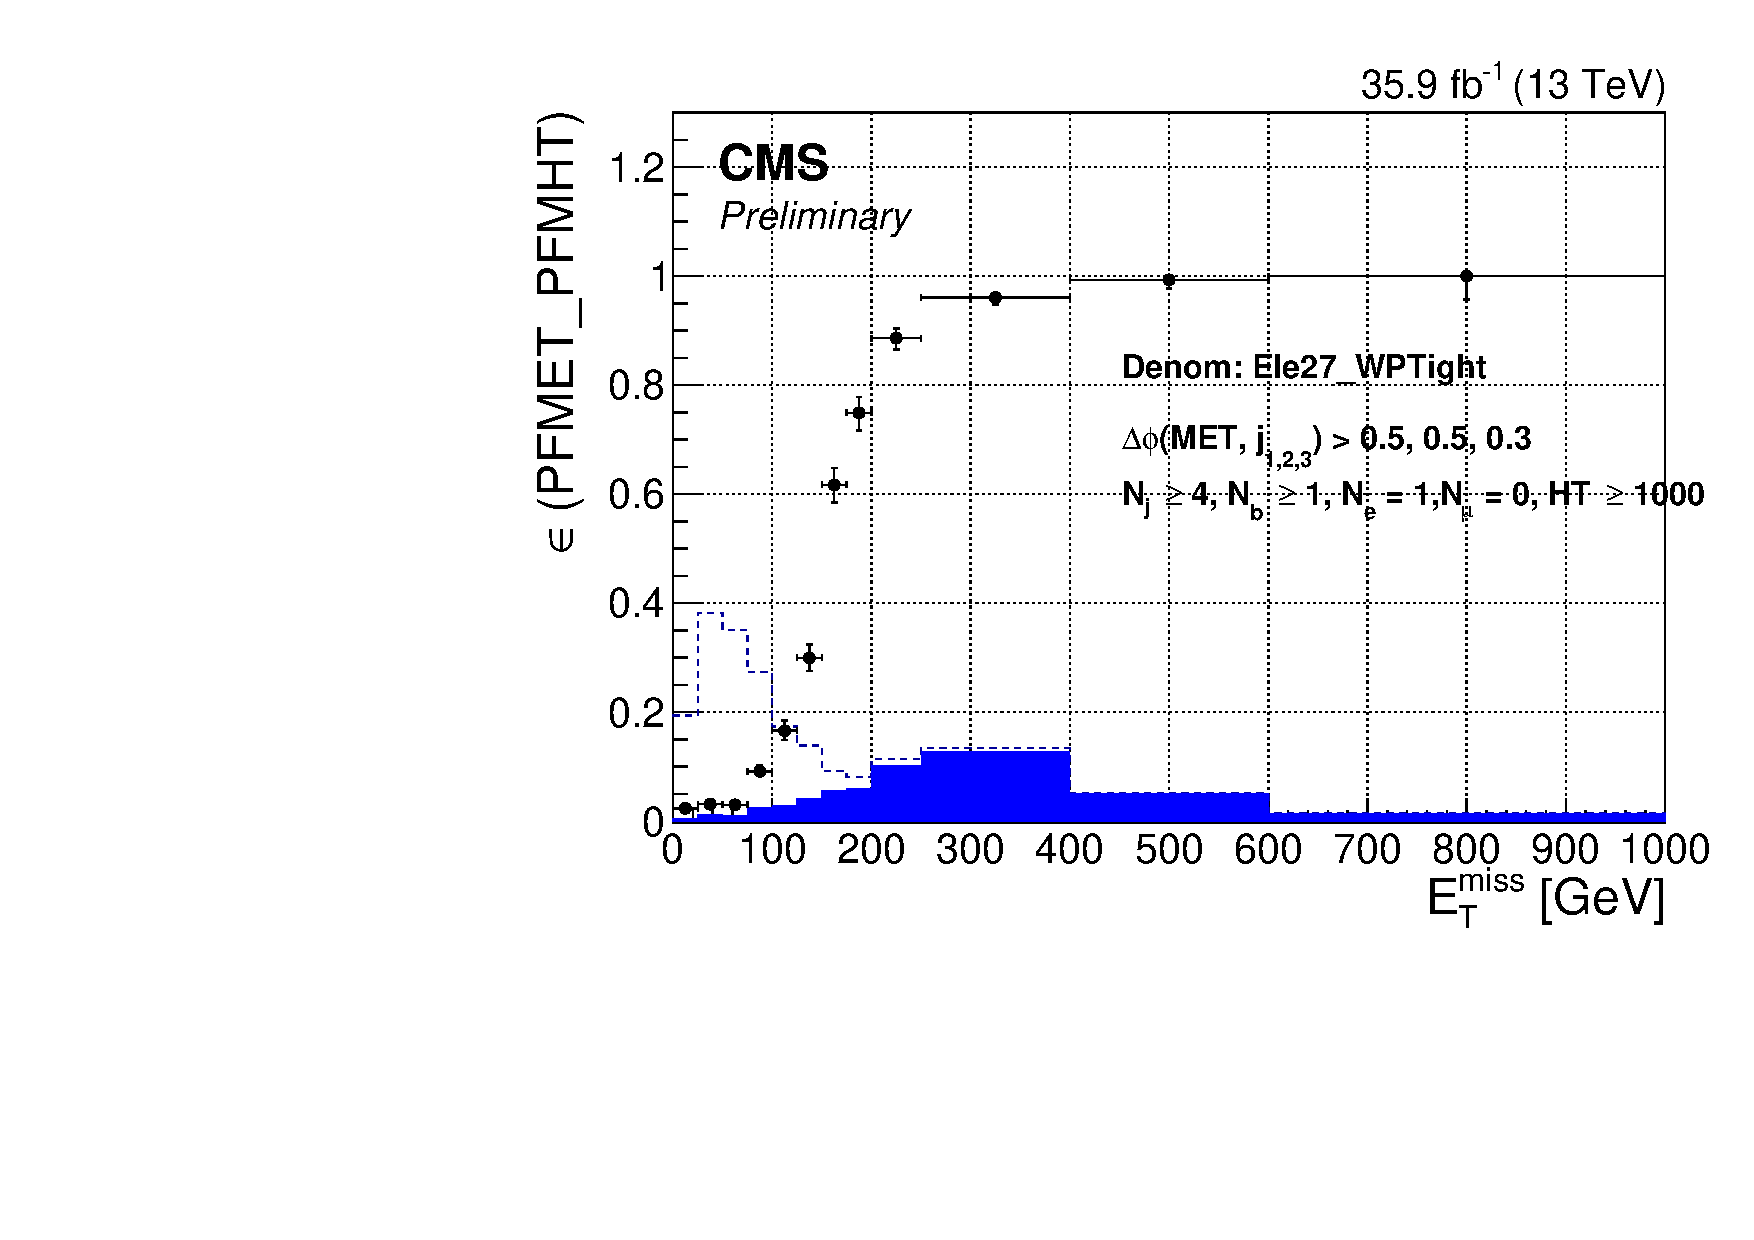
\includegraphics[width=0.49\linewidth]{sections/mc4/EvtSelSBOpt/figures/TrigEle_Stop_TrigMET_HTMore1000_9.pdf}
   \caption{ The trigger efficiency, denote by the black point, as a function
   of the offline \MET for (left) 300 $< \HT <$ 1000 and (right) $\HT >$ 1000.
   The error bar indicates the statistical uncertainty of the trigger
   efficiency. The dash blue line represents the denominator passing the
   selection, while the solid blue histogram represents the numerator where
   the denominator events also trigger the search triggers. }
   \label{fig:TrigMET}
 \end{center}
\end{figure}


Beside measuring the \MET trigger efficiency from the single electron dataset,
the same trigger efficiency can be measured from single muon and HTMHT
dataset. To account for possible bias from different measurements, we will
take the measurement from the single-electron dataset as the nominal and the
variation from the measurements from single-muon and HTMHT dataset as
systematic uncertainty of the trigger efficiency, as shown in
Fig.~\ref{fig:TrigMETSys}. For \MET above 250GeV, we observe similar \MET
trigger efficiency, with systematic uncertainty less than 1\%.

For \MET trigger efficiency measured from single-muon dataset, events are
collected by the single-muon trigger
\begin{itemize}
  \item \texttt{HLT\_Mu50\_v*},
\end{itemize}
with below requrements:
\begin{itemize}
  \item Pass all filters
	\item Leading reconstructed muon with $p_{T}>$ 50GeV
  \item Veto reconstructed electron
  \item $\njets\geq4$
  \item \nbjets $\ge$ 1
  \item \HT $\ge$ 300 GeV
  \item $\Delta\phi(\MET, j_{1,2,3})>$ 0.5, 0.5, 0.3
\end{itemize}
For \MET trigger efficiency measured from HTMHT dataset, events are
collected by the HT triggers
\begin{itemize}
  \item \texttt{HLT\_PFHT200\_v*},
  \item \texttt{HLT\_PFHT250\_v*},
  \item \texttt{HLT\_PFHT300\_v*},
  \item \texttt{HLT\_PFHT350\_v*},
  \item \texttt{HLT\_PFHT400\_v*},
  \item \texttt{HLT\_PFHT475\_v*},
  \item \texttt{HLT\_PFHT600\_v*},
  \item \texttt{HLT\_PFHT800\_v*},
  \item \texttt{HLT\_PFHT900\_v*},
  \item \texttt{HLT\_CaloJet500\_NoJetID\_v*},
\end{itemize}, 
in which \texttt{HLT\_CaloJet500\_NoJetID\_v*} is recommended by Level-1 for
recovering the inefficiency of L1\_HTT trigger during period H data taking.
Event are required to pass below selections:
\begin{itemize}
  \item Pass all filters
  \item Veto reconstructed electron
  \item Veto reconstructed muon
  \item $\njets\geq4$
  \item \nbjets $\ge$ 1
  \item \HT $\ge$ 300 GeV
  \item $\Delta\phi(\MET, j_{1,2,3})>$ 0.5, 0.5, 0.3
\end{itemize}


\begin{figure}[tbp]
 \begin{center}
   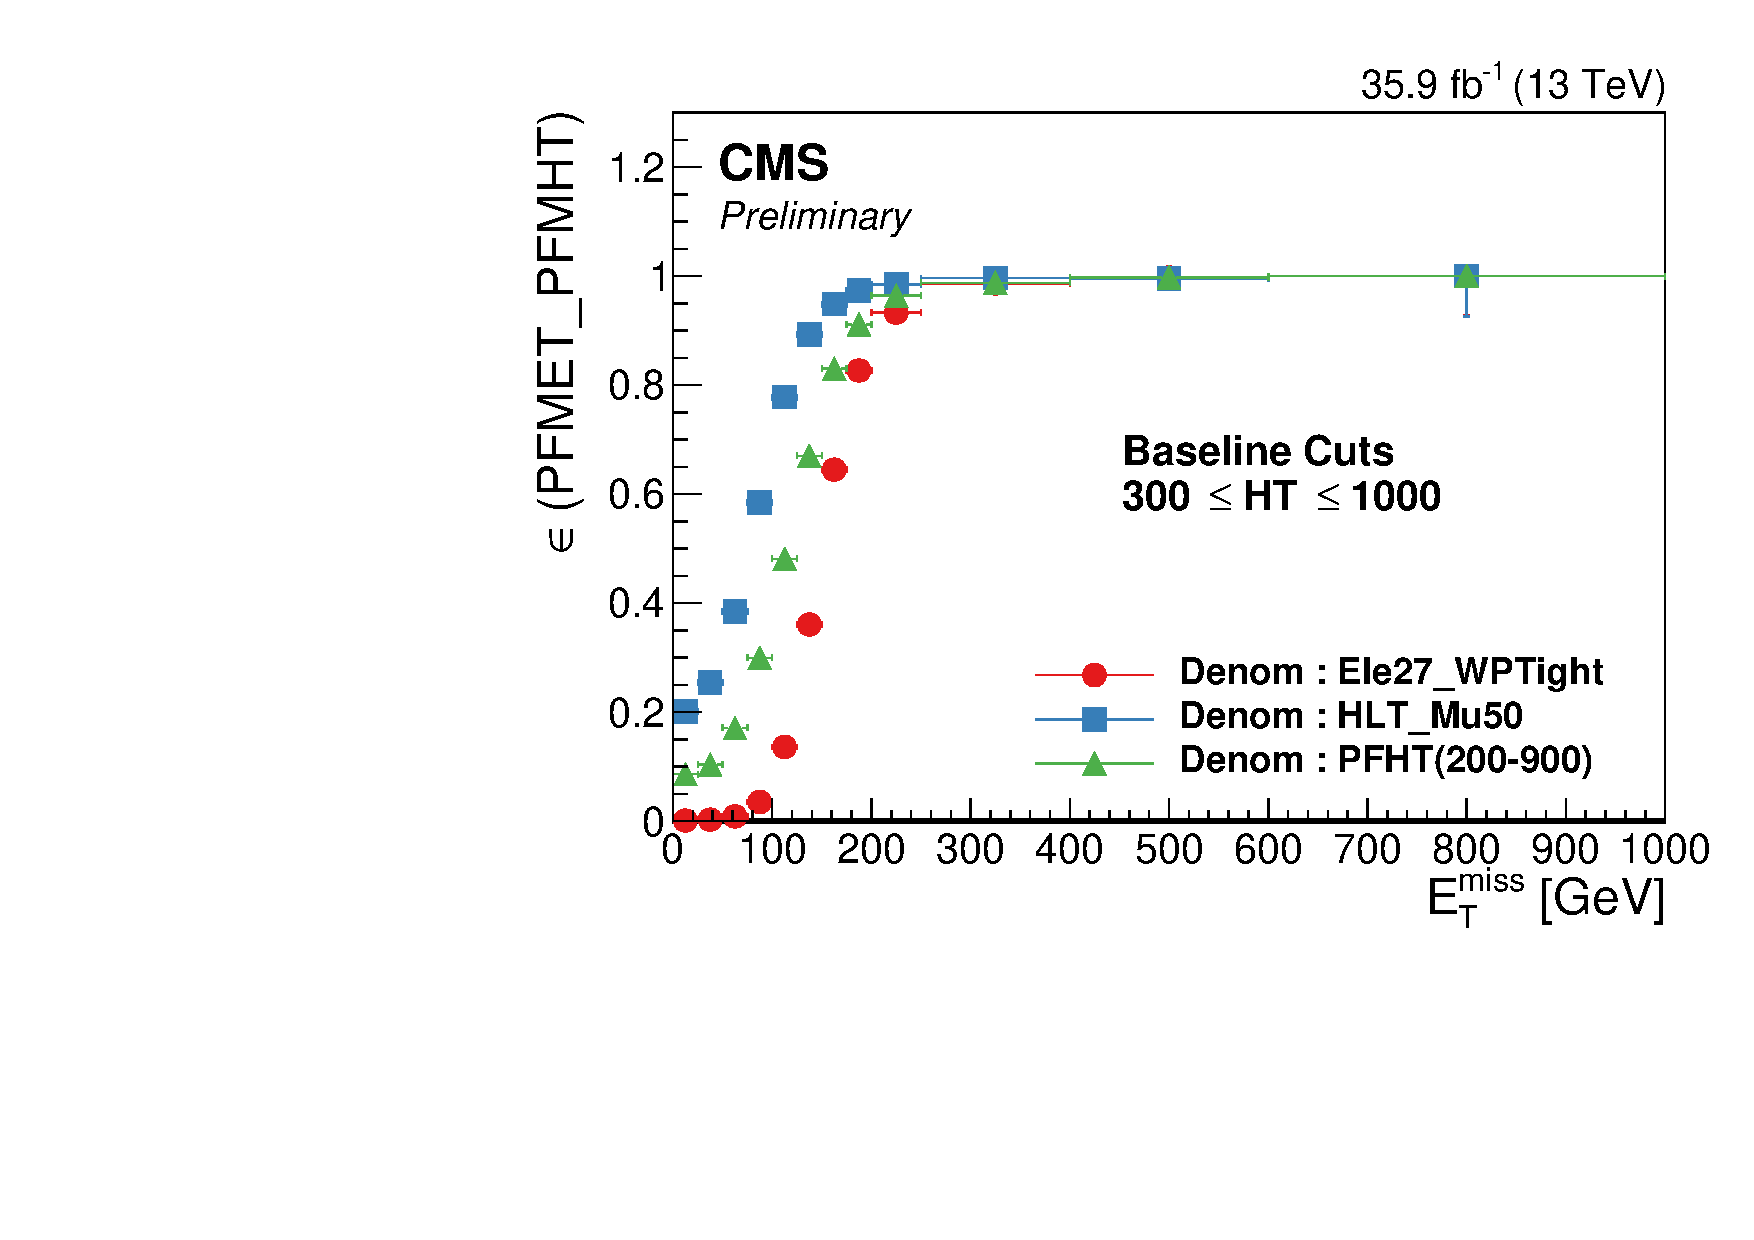
\includegraphics[width=0.49\linewidth]{sections/mc4/EvtSelSBOpt/figures/TrigMET_HTLess1000.pdf}
   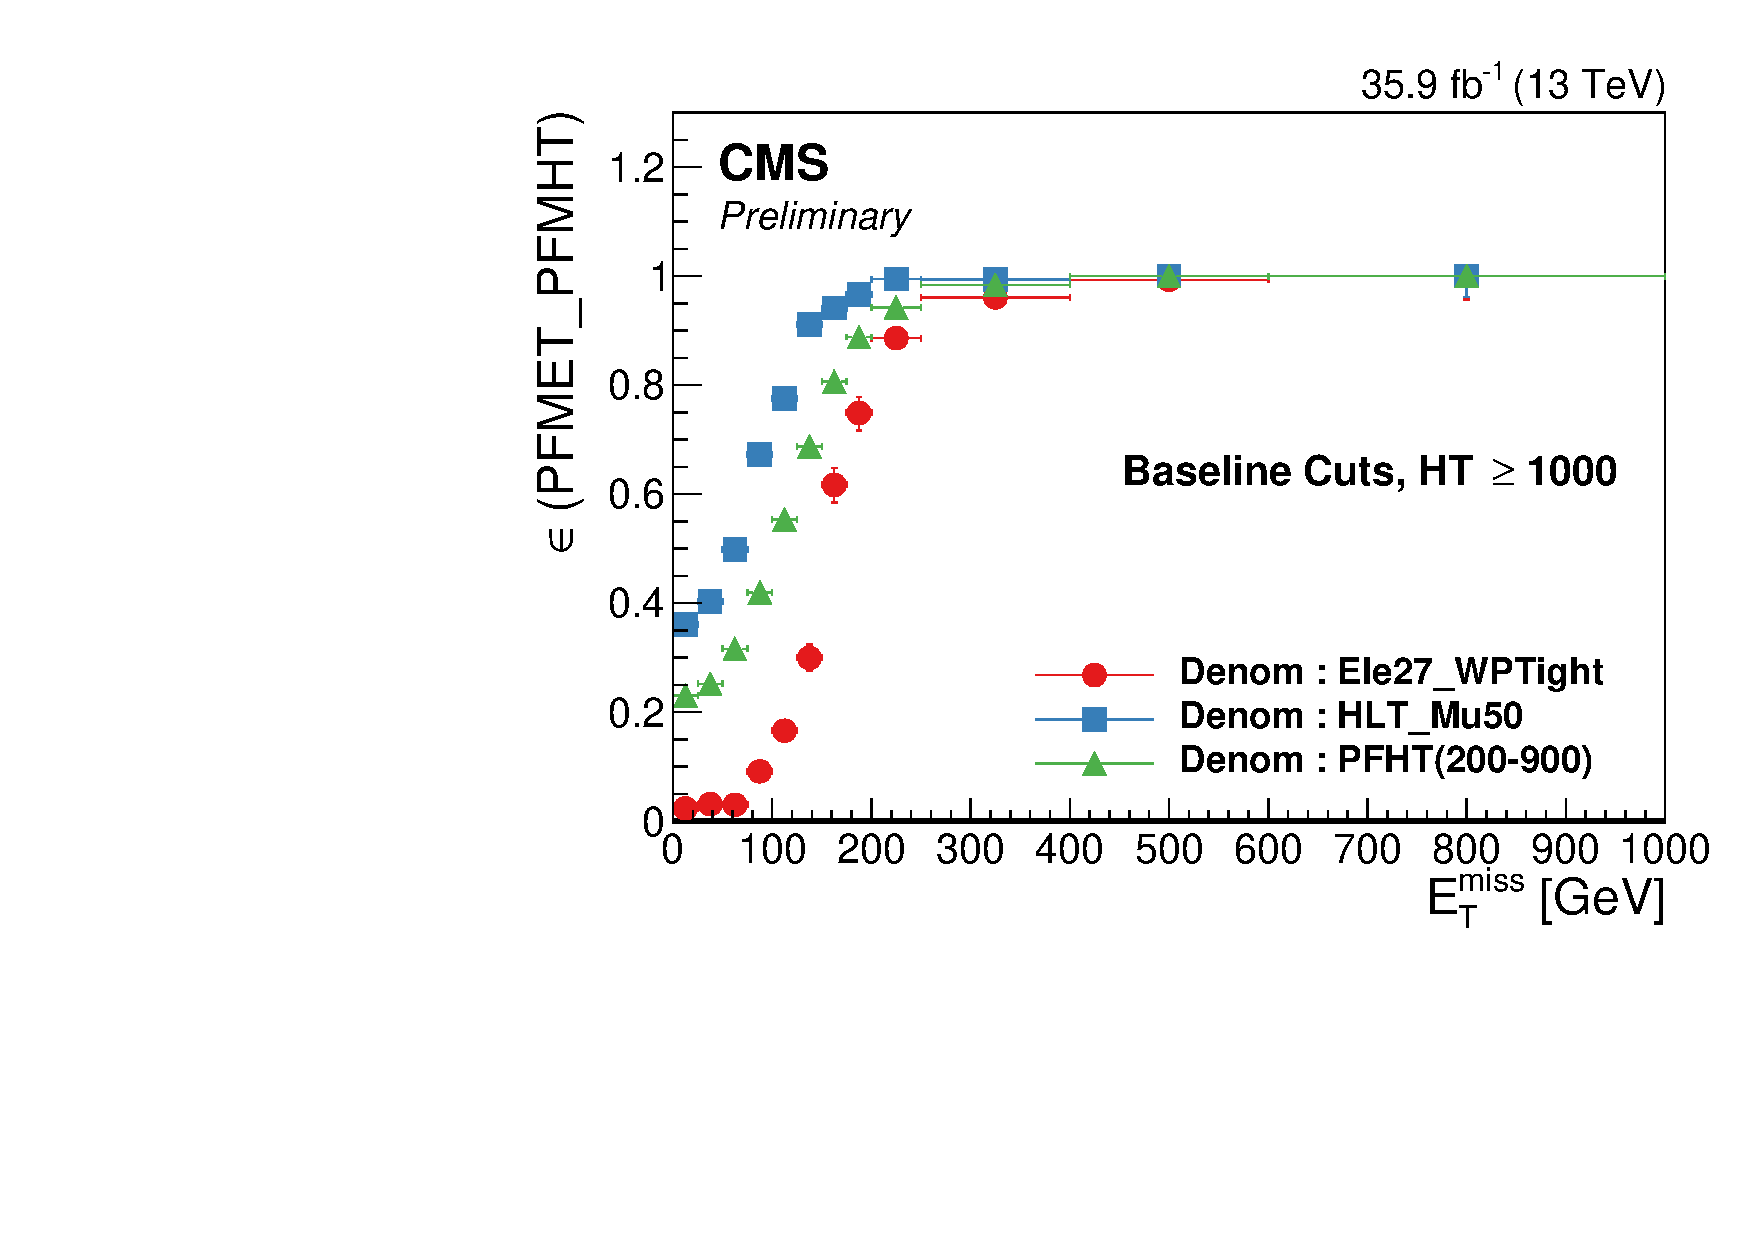
\includegraphics[width=0.49\linewidth]{sections/mc4/EvtSelSBOpt/figures/TrigMET_HTMore1000.pdf}
   \caption{ The trigger efficiency, denote by the black point, as a function
   of the offline \MET for (left) 300 $< \HT <$ 1000 and (right) $\HT >$ 1000.
   The error bar indicates the statistical uncertainty of the trigger
   efficiency. The blue square represents efficiency measured with
   single-muon dataset.  The red point represents efficiency measured
   with single-electron dataset while the green triangle represents
   efficiency measured with HT dataset.}
   \label{fig:TrigMETSys}
 \end{center}
\end{figure}

We also checked the trigger efficiency as a function of number of AK4 jets and
$b$-tagged jets, after requiring \MET $>$ 250GeV, as shown in
Fig.~\ref{fig:TrigMETJets}. Similar efficiencies are observed from different
measurements.

\begin{figure}[tbp]
 \begin{center}
   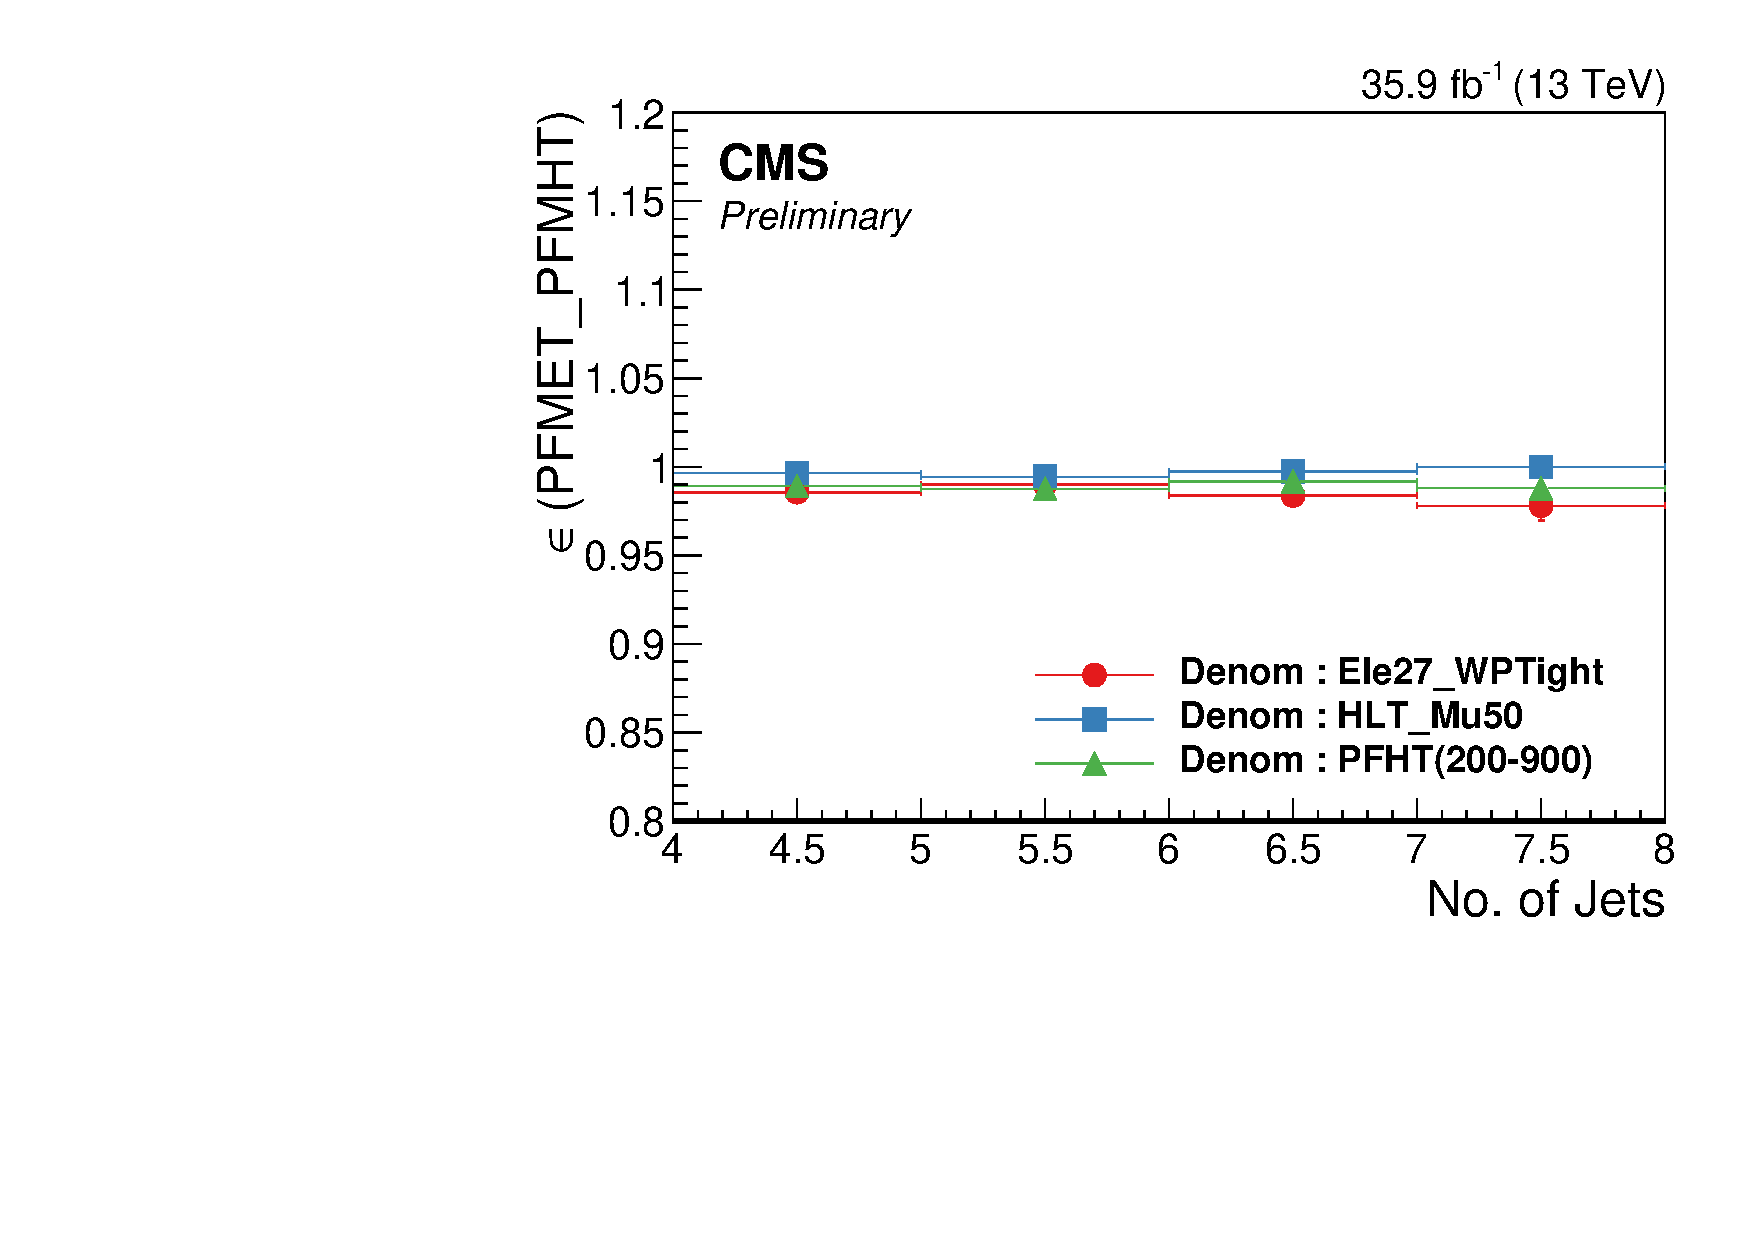
\includegraphics[width=0.49\linewidth]{sections/mc4/EvtSelSBOpt/figures/TrigNJets.pdf}
   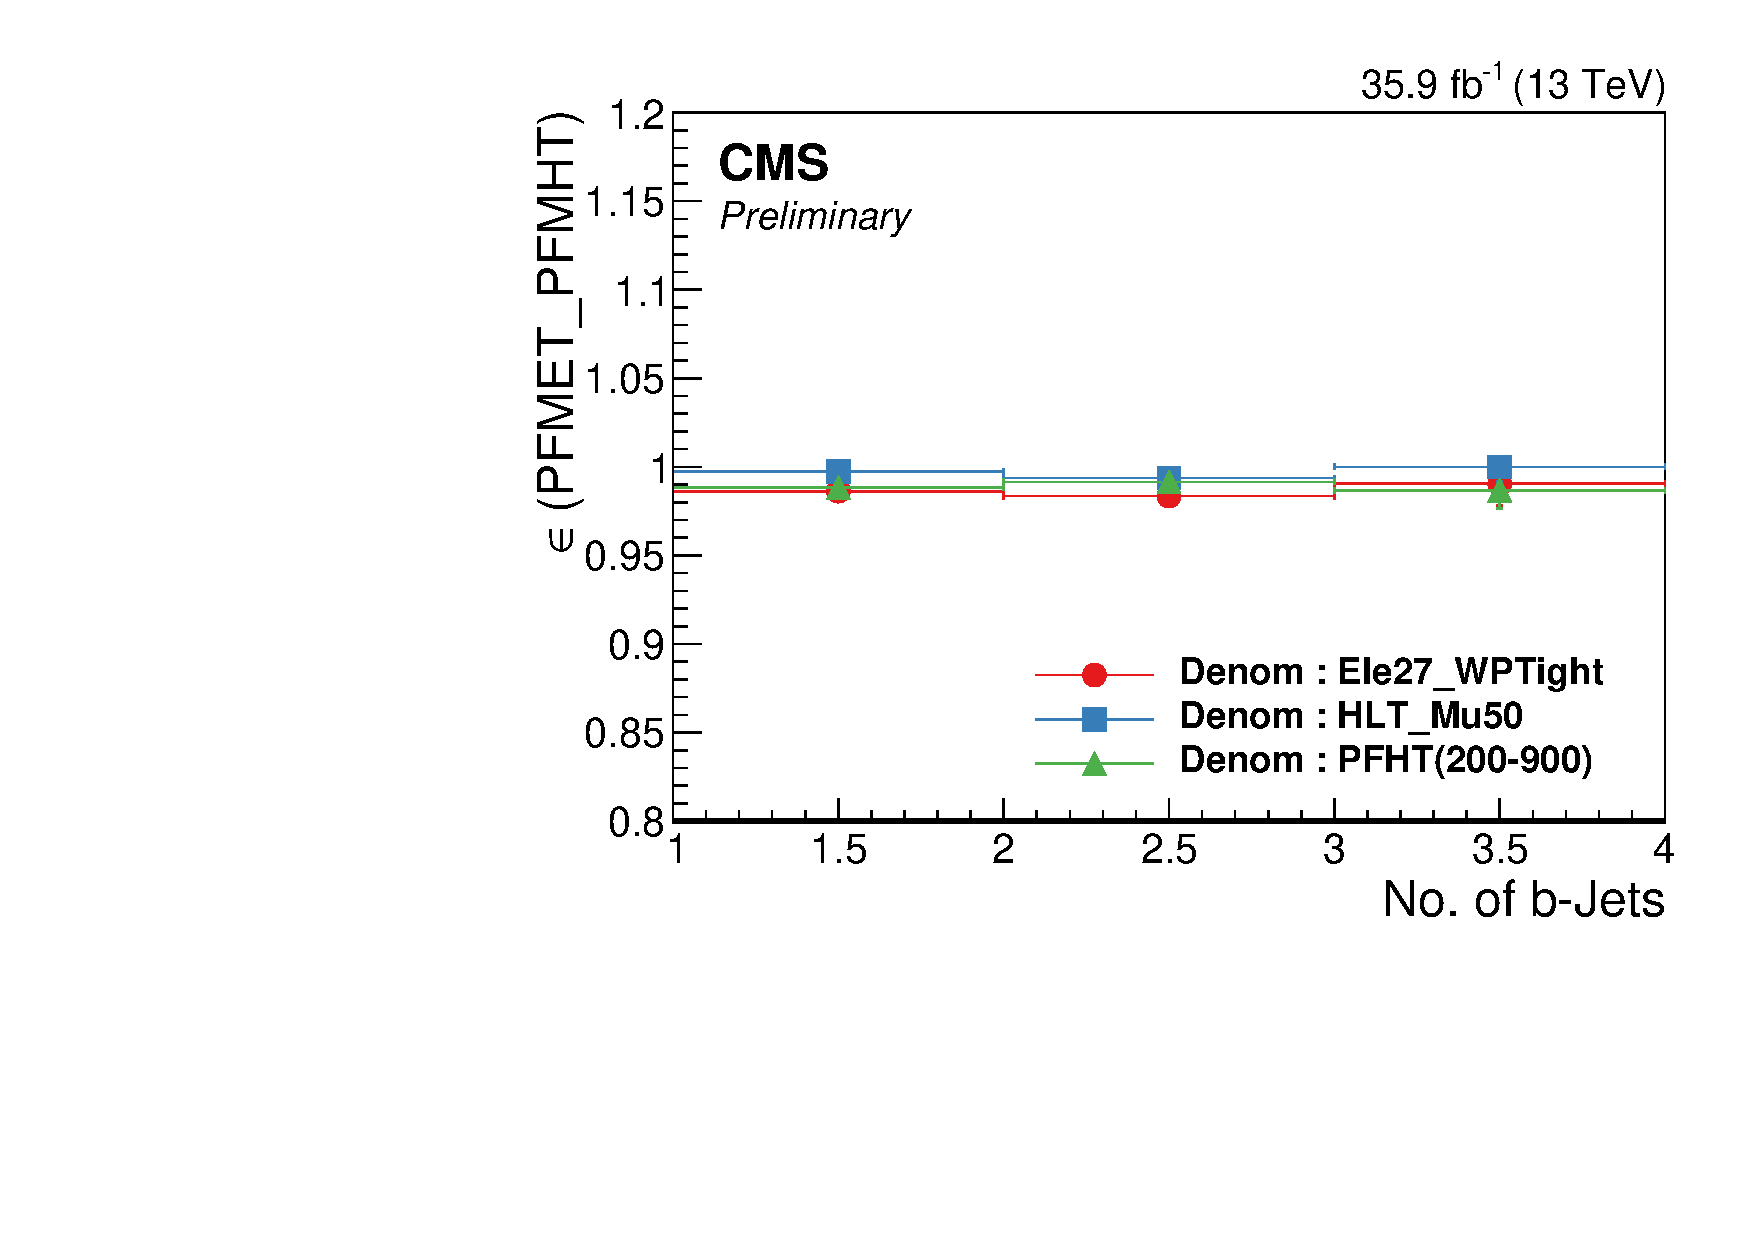
\includegraphics[width=0.49\linewidth]{sections/mc4/EvtSelSBOpt/figures/TrigNBs.pdf}
   \caption{ The trigger efficiency, denote by the black point, as a function
		 of the offline (left) number of jets with $p_{T}>$ 30 GeV and (right) number
		 of $b$-tagged jets with $p_{T}>$ 30GeV. The error bar indicates the
   statistical uncertainty of the trigger efficiency. The blue square
   represents efficiency measured with single-muon dataset.  The red point
   represents efficiency measured with single-electron dataset while the green
   triangle represents efficiency measured with HT dataset.}
   \label{fig:TrigMETJets}
 \end{center}
\end{figure}

The QCD background are estimated using the events triggered by search
triggers, but with cuts to select the QCD-enriched region. Since there are no
real \MET in QCD sample, the \MET trigger efficiency in the QCD-enriched
region would be different from the search region in the low \MET region. A
measurement of the trigger efficiency in the QCD-enriched region is carried
out in the HTMHT dataset to avoid bias. Events are required to pass the
similar cuts as the search trigger efficiency measurement, except an inverted
$\Delta\phi(\MET, j_{1,2,3})$ requirement as blow:
\begin{itemize}
  \item Pass all filters
  \item Veto reconstructed electron
  \item Veto reconstructed muon
  \item $\njets\geq4$
  \item \nbjets $\ge$ 1
  \item \HT $\ge$ 300 GeV
  \item $\Delta\phi(\MET, j_{1,2,3})<$ 0.5, 0.5, 0.3
\end{itemize}
The trigger efficiency is measured as a function of the offline \MET and showed in Fig.~\ref{fig:TrigMETQCD}.
\begin{figure}[tbp]
 \begin{center}
   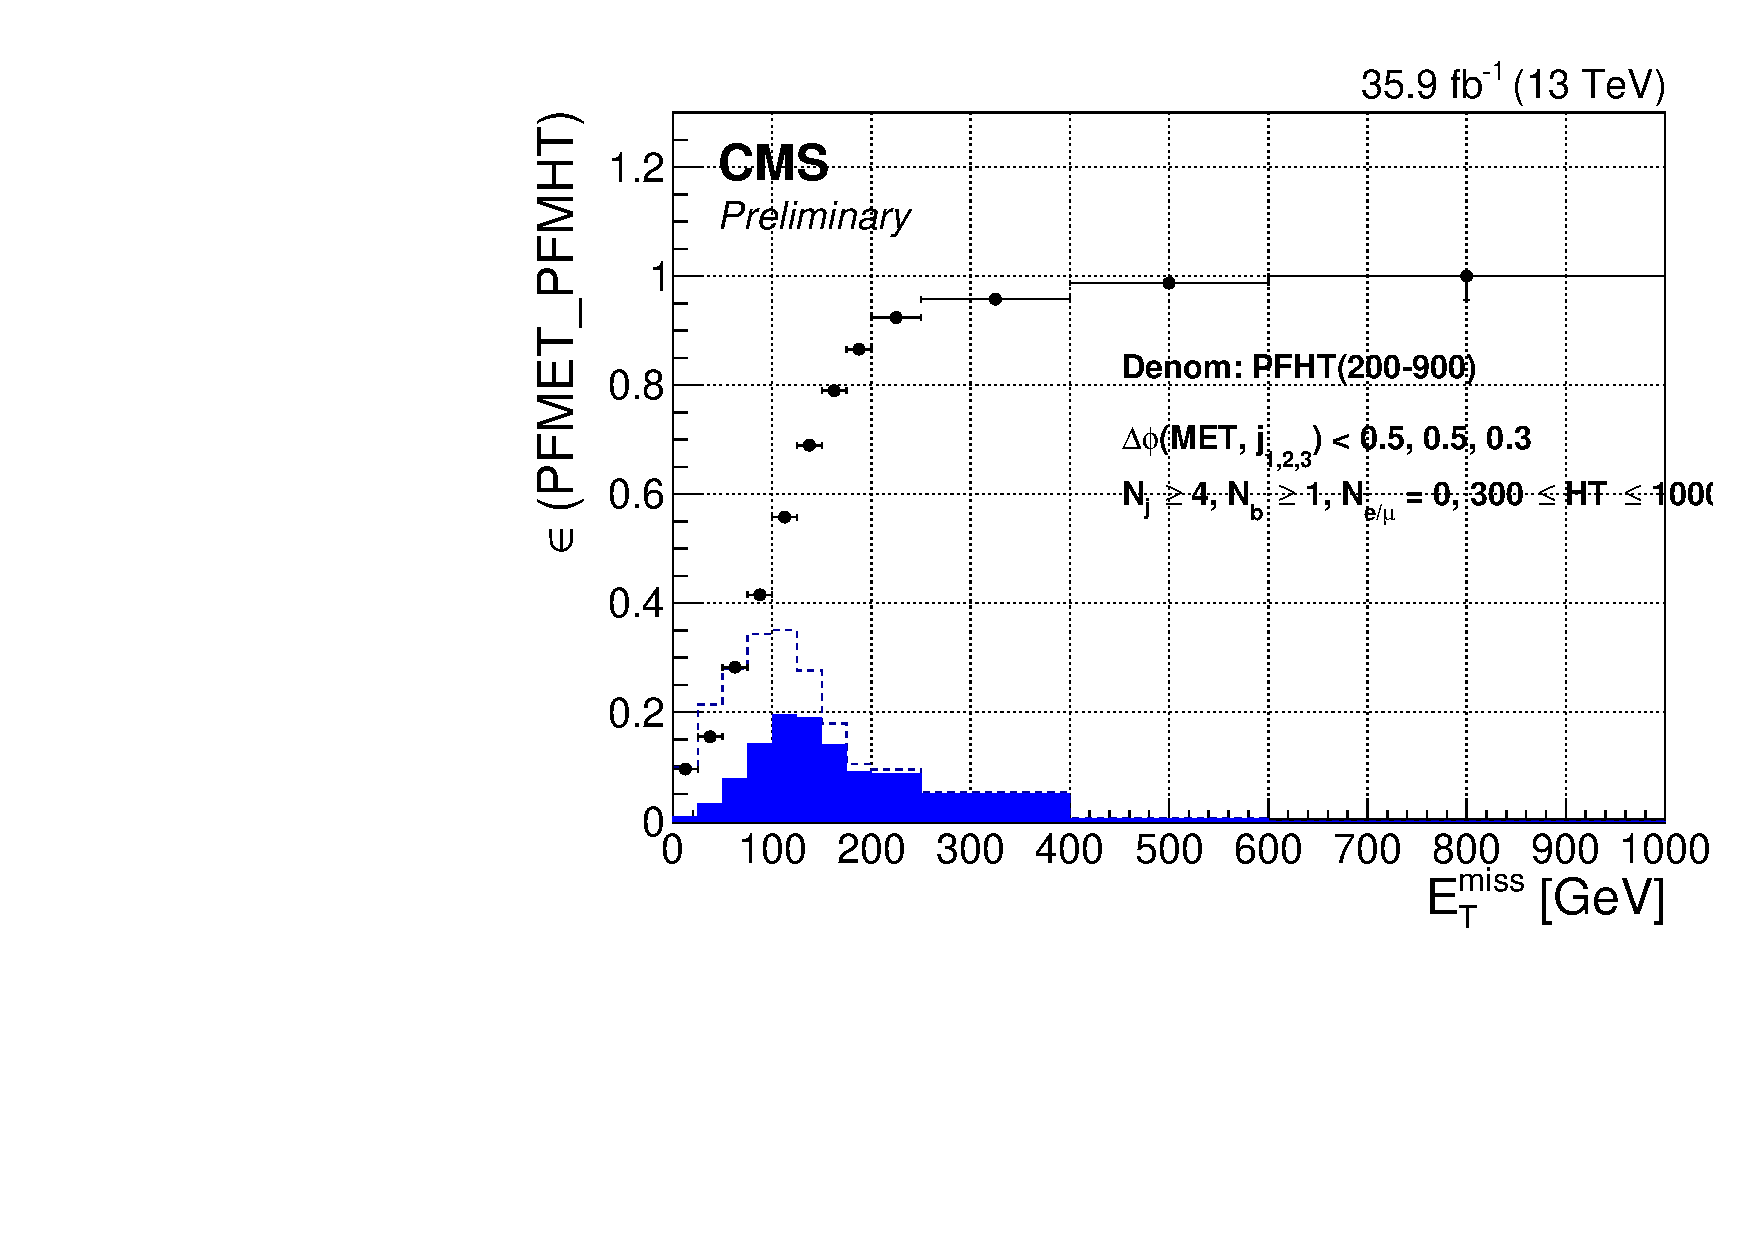
\includegraphics[width=0.49\linewidth]{sections/mc4/EvtSelSBOpt/figures/TrigHT_QCD_TrigMET_HTLess1000_9.pdf}
   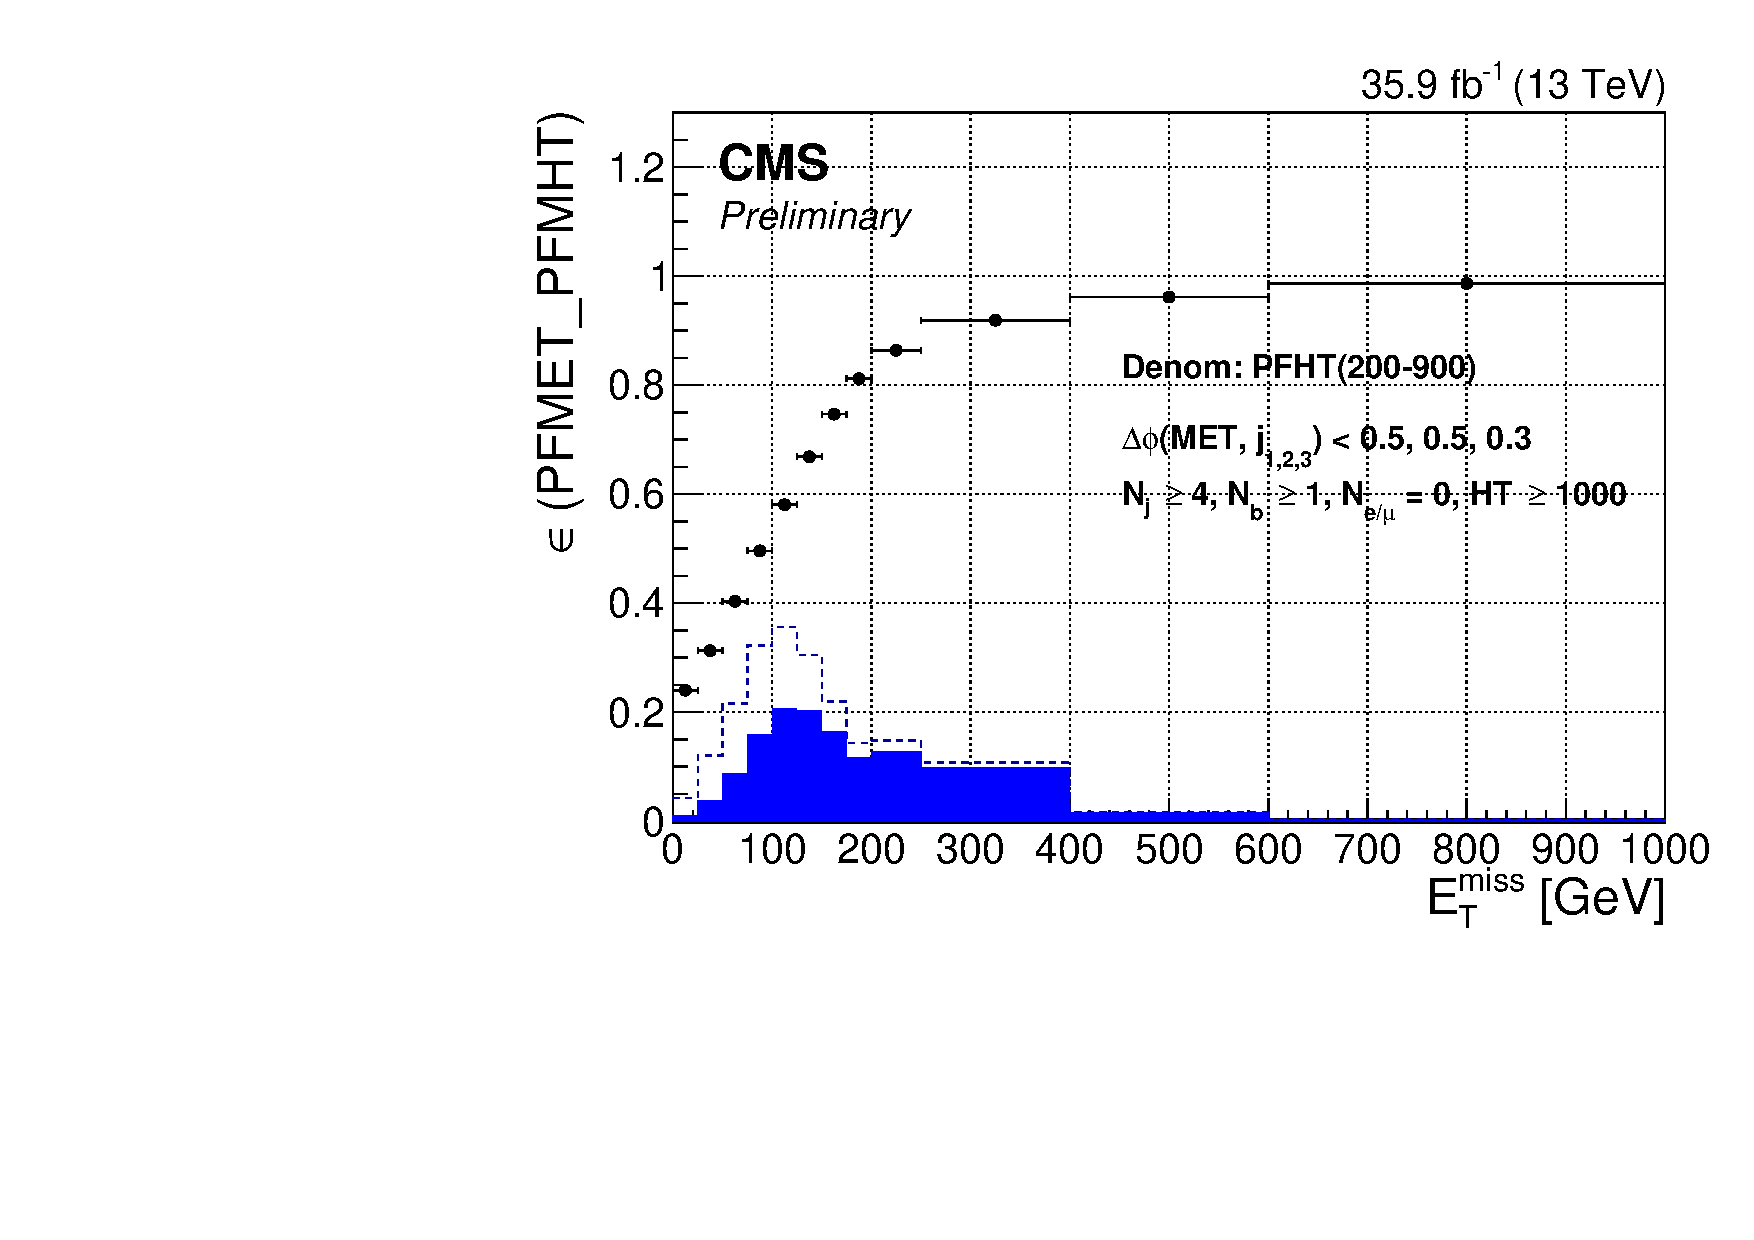
\includegraphics[width=0.49\linewidth]{sections/mc4/EvtSelSBOpt/figures/TrigHT_QCD_TrigMET_HTMore1000_9.pdf}
   \caption{ The trigger efficiency, denote by the black point, as a function
   of the offline \MET for (left) 300 $< \HT <$ 1000 and (right) $\HT >$ 1000.
   The error bar indicates the statistical uncertainty of the trigger
   efficiency. The dash blue line represents the denominator passing the
   selection, while the solid blue histogram represents the numerator where
   the denominator events also trigger the search triggers. }
   \label{fig:TrigMETQCD}
 \end{center}
\end{figure}

Events in the di-muon control sample, which is used for the estimation of the
background from events in which a Z boson decays into neutrinos, are
collected by the single muon trigger. 
\begin{itemize}
  \item \texttt{HLT\_IsoMu24\_eta2p1\_v*}.
  \item \texttt{HLT\_IsoTKMu24\_eta2p1\_v*}.
  \item \texttt{HLT\_Mu50\_eta2p1\_v*}.
\end{itemize}
The trigger efficiencies are measured in the single-electron sample with below selections:
\begin{itemize}
  \item Pass all filters
	\item Leading reconstructed electron with $p_{T}>$ 30GeV
  \item At least one reconstructed muon
  \item $\njets\geq4$
  \item \nbjets $\ge$ 1
  \item \HT $\ge$ 300 GeV
\end{itemize}

The measured single muon trigger efficiency as a function of the reconstructed
leading muon $p_{T}$ and $\eta$ is shown in Fig.~\ref{fig:TrigMuon}.
The muon trigger efficiency is also measured in the HT and MET dataset as
cross checks. We also checked the benefits of adding the double muon triggers
\begin{itemize}
  \item \texttt{HLT\_Mu17\_TrkIsoVVL\_Mu8\_TrkIsoVVL\_DZ\_v*}.
  \item \texttt{HLT\_Mu17\_TrkIsoVVL\_TkMu8\_TrkIsoVVL\_DZ\_v*}.
\end{itemize}.
We do observe a small gain of muon efficiencies as shown in
Fig.~\ref{fig:TrigMuon}, but no beneficial for the $Z \rightarrow \nu \nu$ background method.

\begin{figure}[tbp]
 \begin{center}
   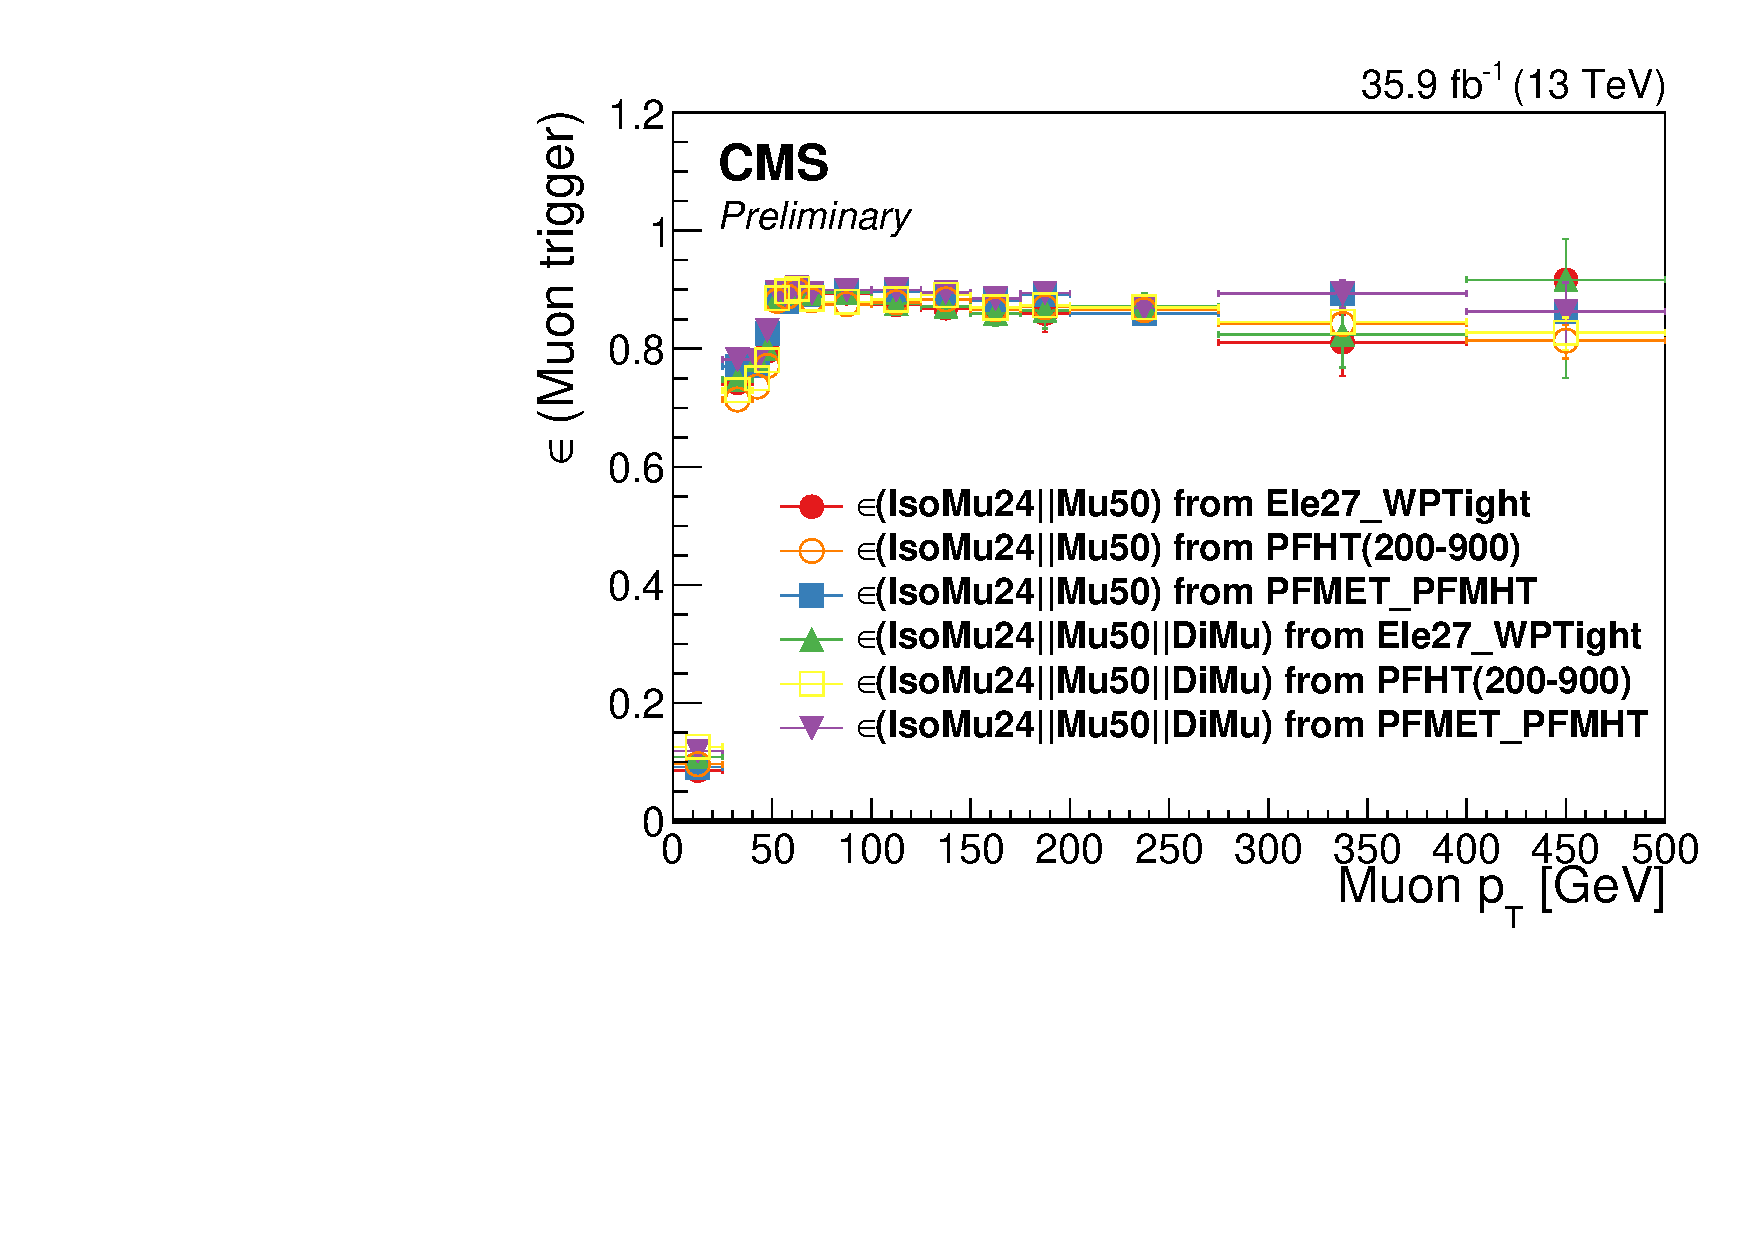
\includegraphics[width=0.49\linewidth]{sections/mc4/EvtSelSBOpt/figures/MuonPT.pdf}
   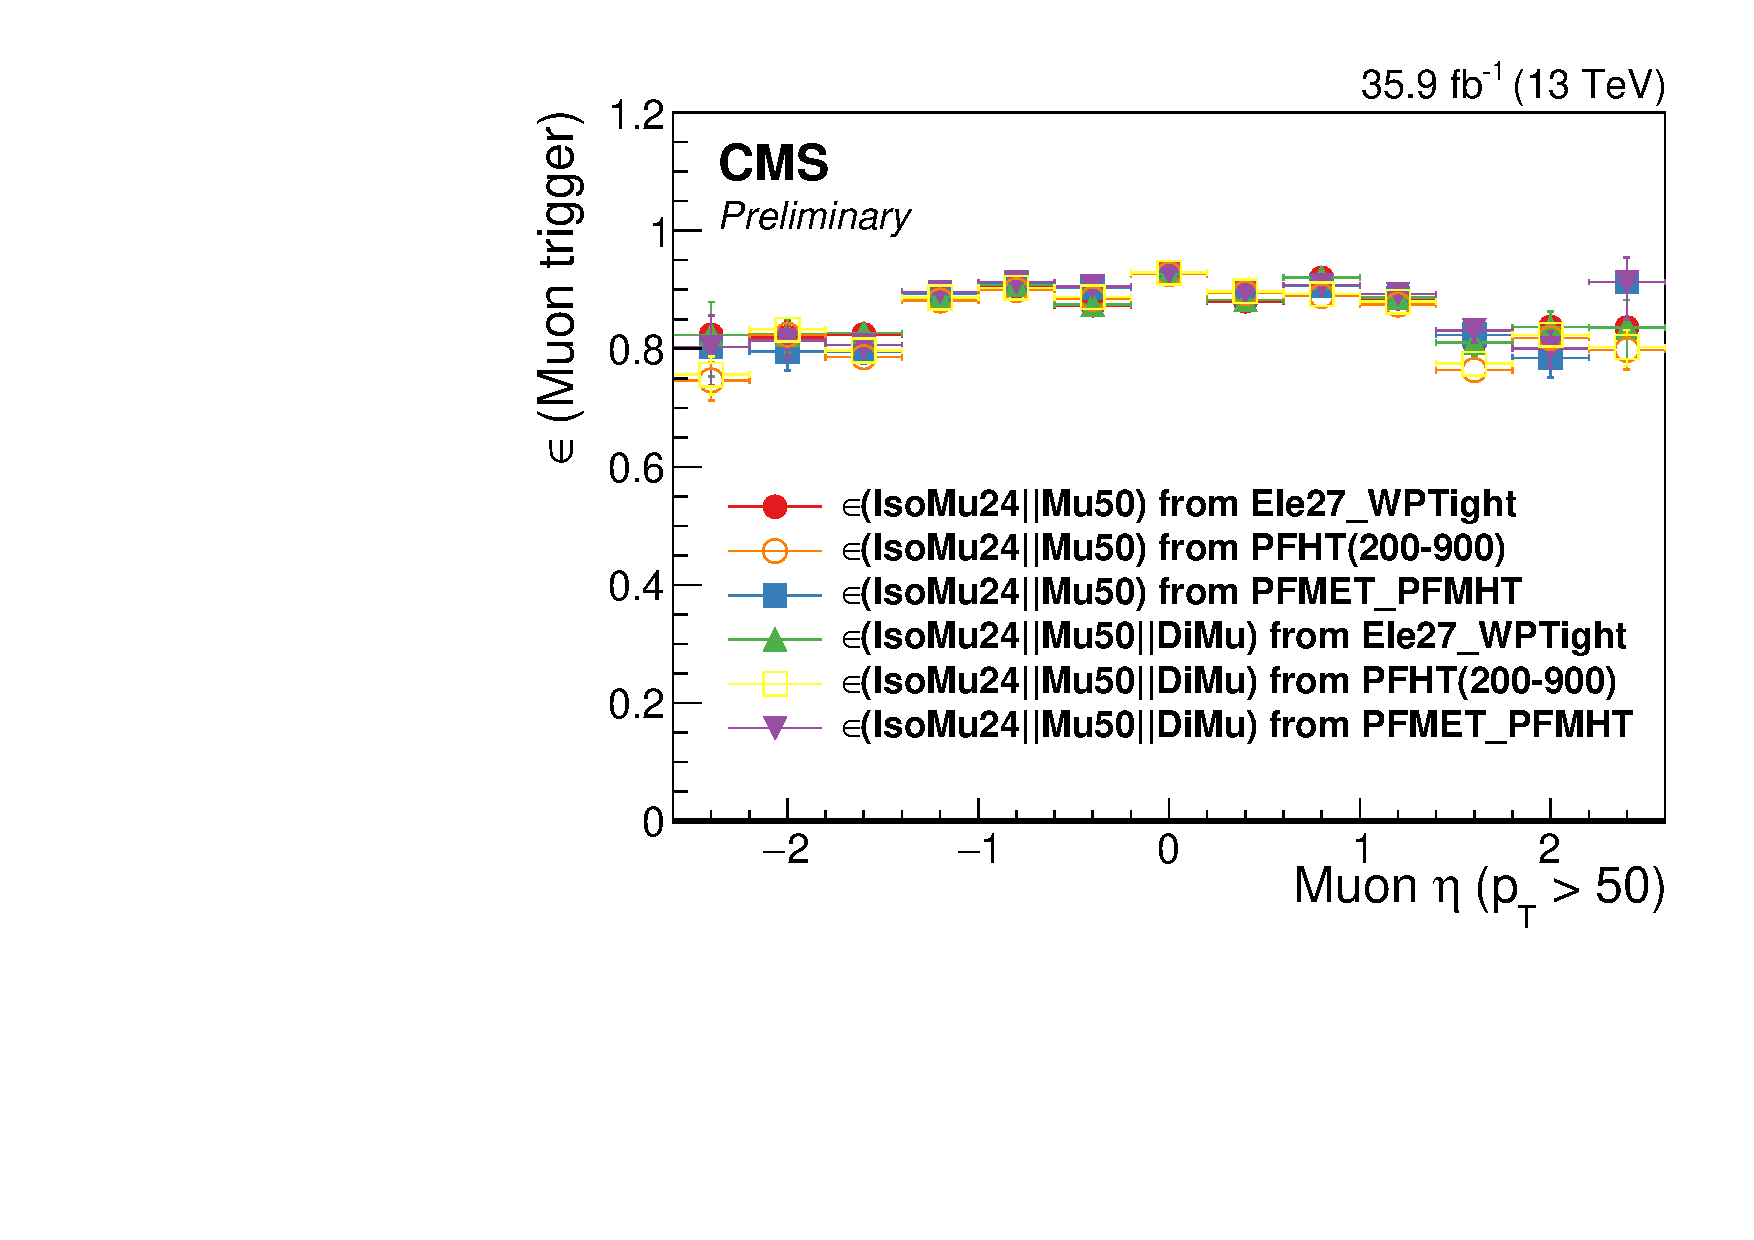
\includegraphics[width=0.49\linewidth]{sections/mc4/EvtSelSBOpt/figures/MuonEta.pdf}
   \caption{ The trigger efficiency as a function of the offline leading Muon
	 (left) $p_{T}$ and (right) $\eta$.}
   \label{fig:TrigMuon}
 \end{center}
\end{figure}

We also checked the trigger efficiency as a function of number of AK4 jets and
$b$-tagged jets, after requiring leading muon with $p_{T}>$ 50GeV, as shown in
Fig.~\ref{fig:TrigMuonJets}. We observed similar efficiency from different
measurements.
\begin{figure}[tbp]
 \begin{center}
   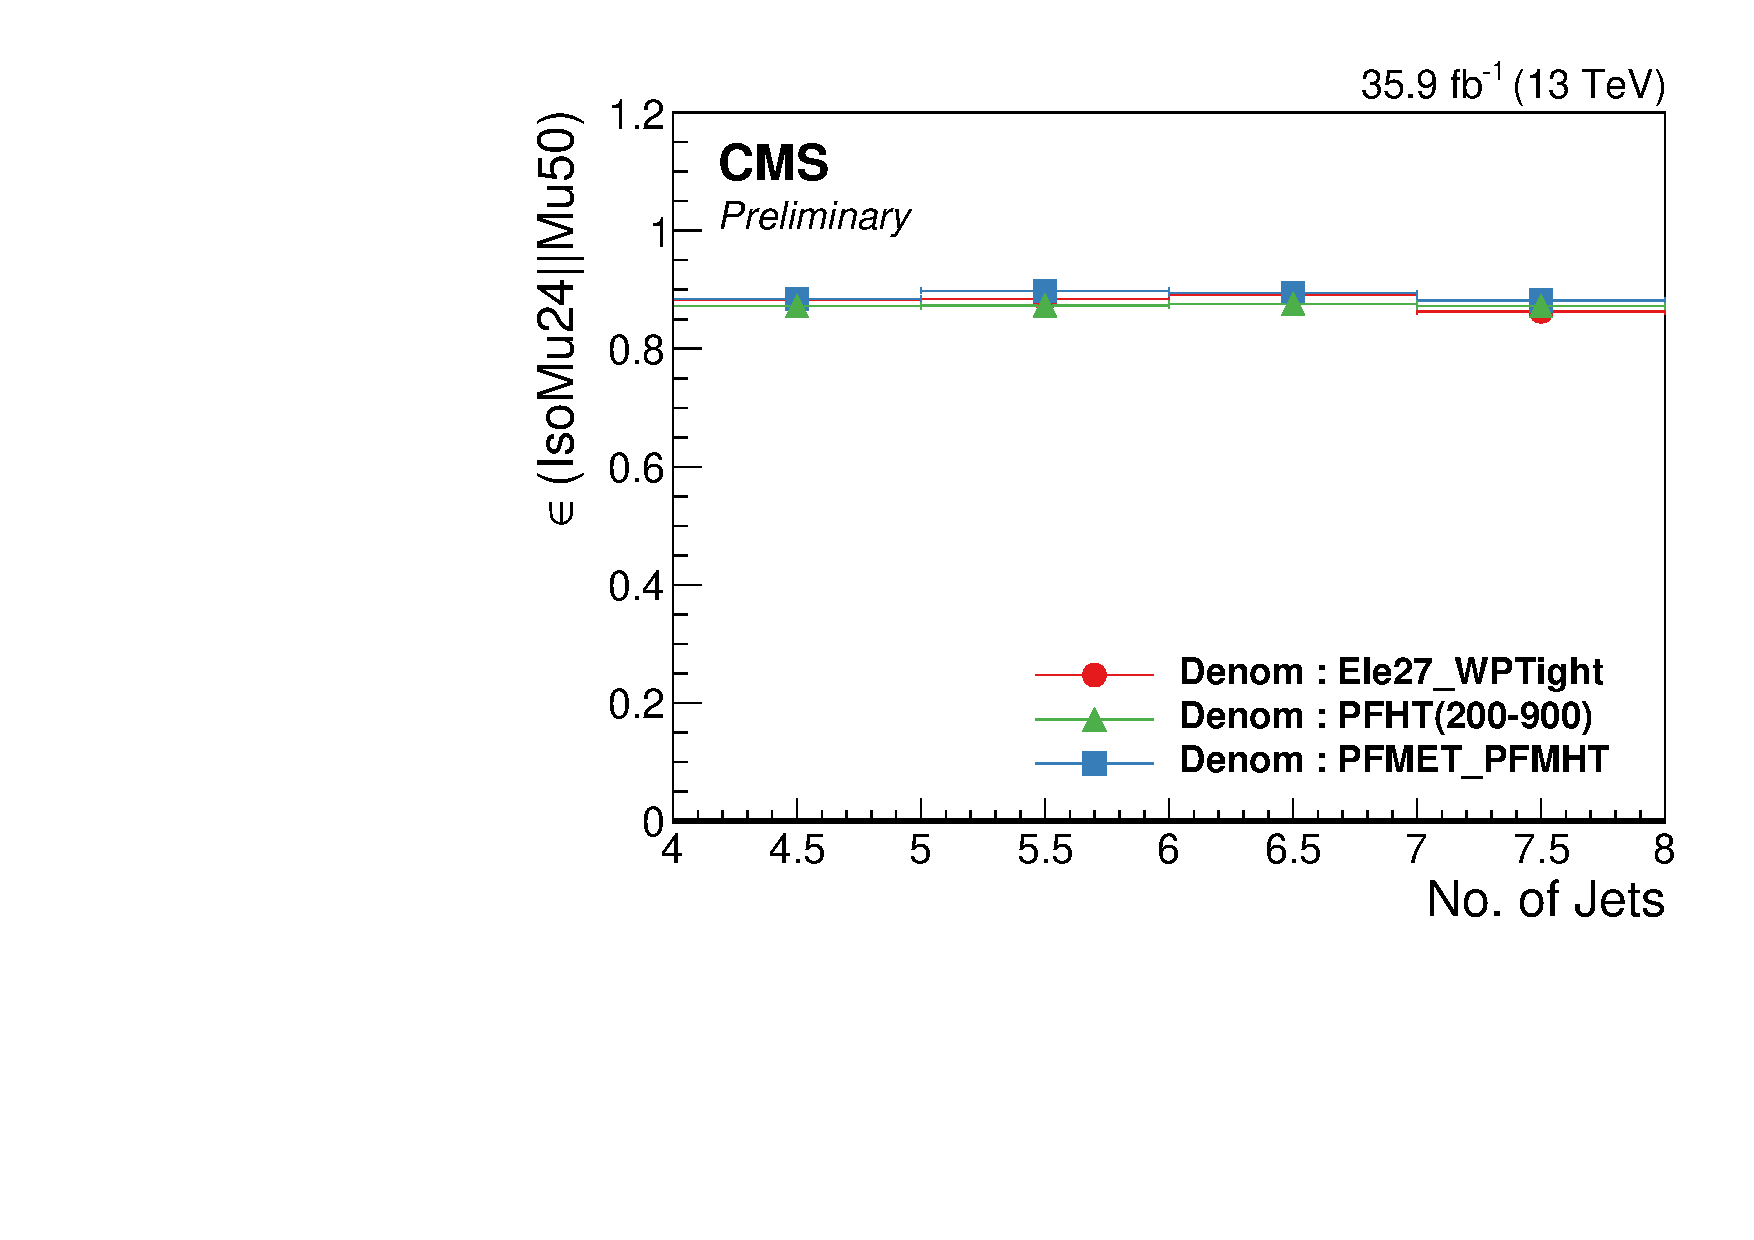
\includegraphics[width=0.49\linewidth]{sections/mc4/EvtSelSBOpt/figures/MuonNJets.pdf}
   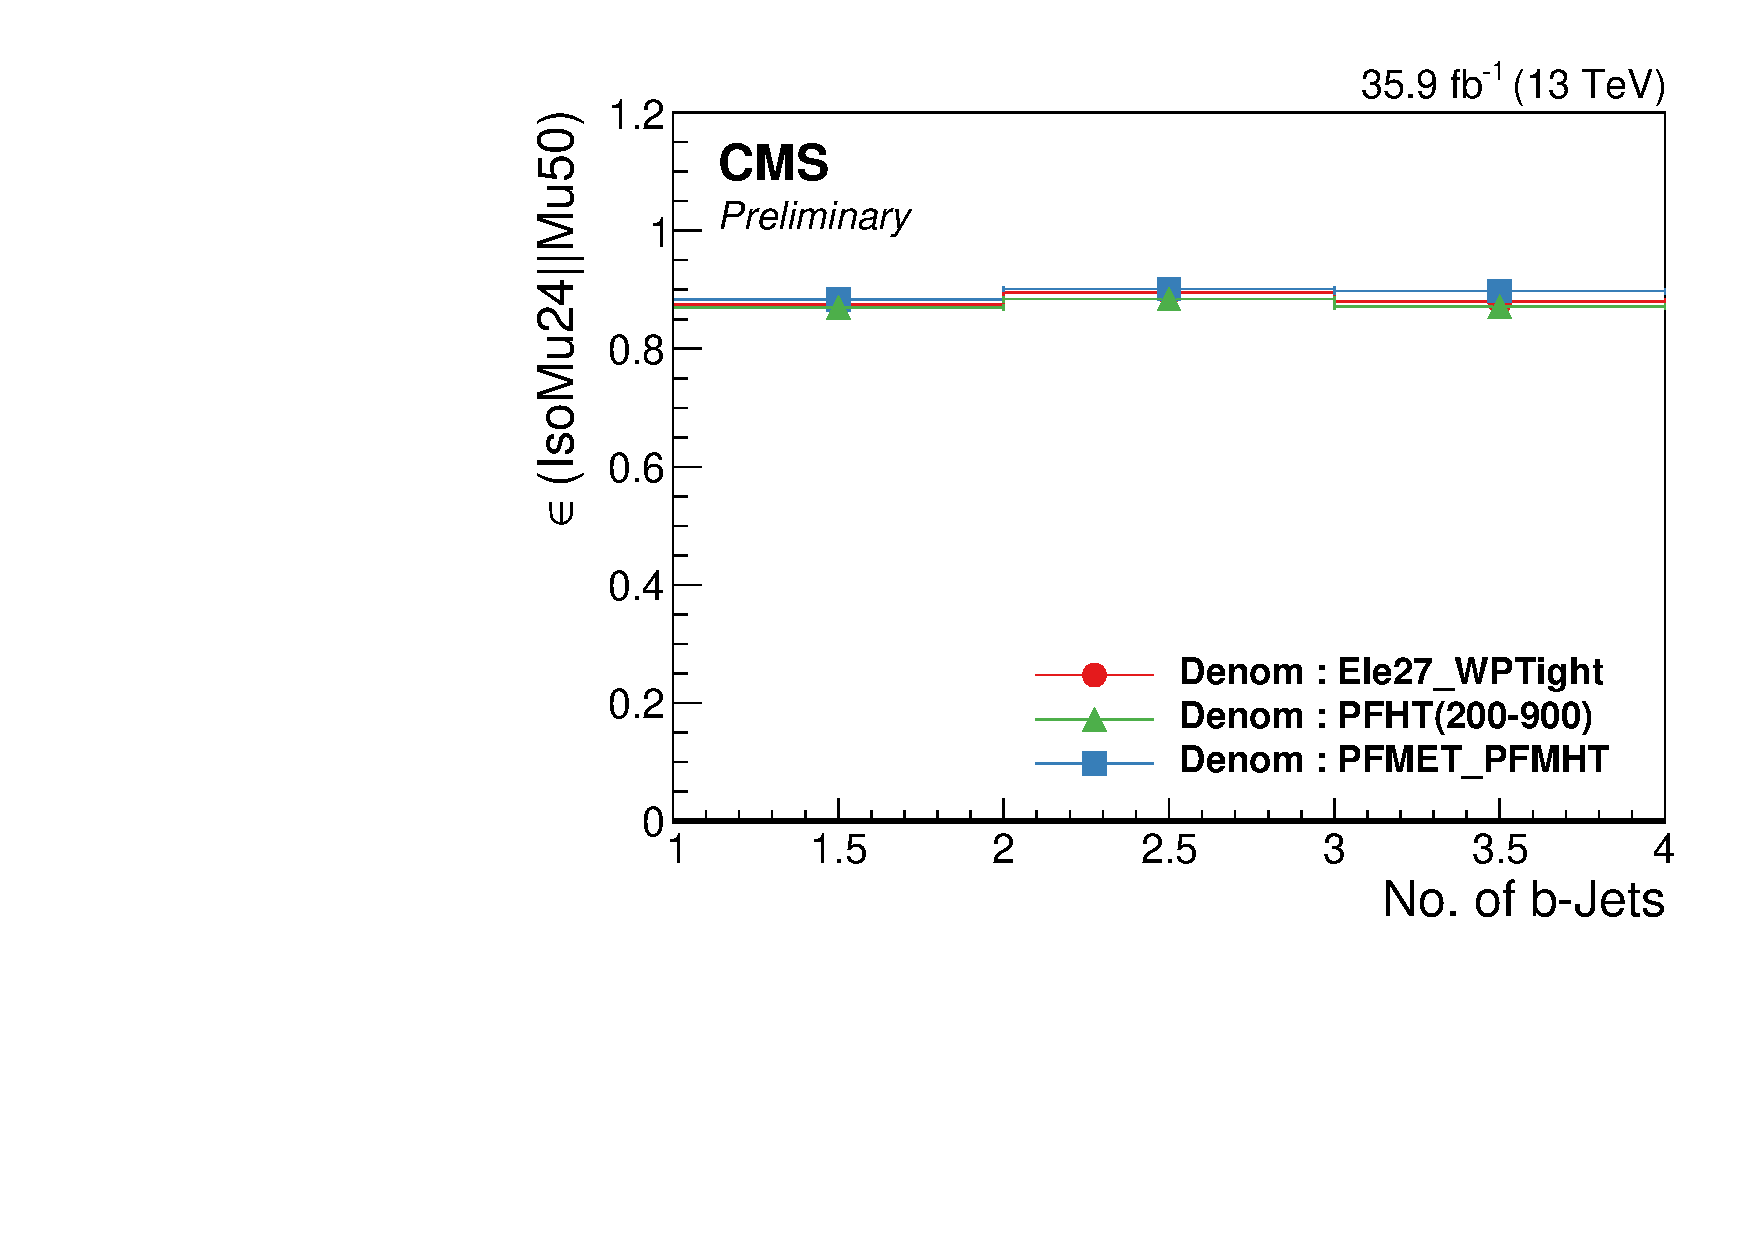
\includegraphics[width=0.49\linewidth]{sections/mc4/EvtSelSBOpt/figures/MuonNBs.pdf}
   \caption{ The trigger efficiency as a function of the offline (left) number
		 of jets with $p_{T}>$ 30 GeV and (right) number of $b$-tagged jets with $p_{T}$
		 $>$ 30GeV, with leading reconstructed muon $p_{T}$ above 50GeV from the
   single-muon trigger. The red point denote the measurement from
   single-electron dataset. The green triangle represents measurement from HT
   dataset, while blue square represents measurement from MET dataset.}
   \label{fig:TrigMuonJets}
 \end{center}
\end{figure}

\subsection{Pre-selection}
\label{sec:pre-selection}

The search looks at multijet events, with b-jets decaying from top quarks, 
large \MET and no leptons. Initially, a loose baseline selection is applied 
in \MET, \HT, \njets and \nbjets. %As illustrated in Tab.~\ref{tab:cutflowMC}, 
This baseline selection preserves 2-20\% of the signal events. 
The events passing the baseline selection are classified into search regions
defined in terms of \ntops, \nbjets, \MET, \HT and \MTTwo.

The following cuts define the baseline selection:

\begin{itemize}
\item Pass all filters that remove detector- and beam-related noise: 
  \begin{itemize}
    \item HBHE noise filter, 
    \item HBHEiso noise filter, 
    \item Ecal dead cell trigger primitive filter,
    \item Primary vertex filter,
    \item Bad EE super crystal filter,
    \item Global tight beam halo filter,
%    \item Fourth bad EE super crystal filter,
    \item Bad muon filter,
    \item Bad charged hadron filter,
    \item Loose JetID event filter.
  \end{itemize}

\item $\njets\geq4$:

%Since the stop is produced in pairs (R-parity conservation) and each one decays to two top quarks, the all-hadronic final state must contain at least four jets. 
Since the stop is produced in pairs and each stop decays to a top and a LSP, the all-hadronic final state will contain 6 jets. Not all the jets pass the selection cuts, therefore we only require at least four jets.
Jets are reconstructed with the Particle Flow (PF) technique
and clustered with the anti-$k_\mathrm{T}$ algorithm with a resolution 
parameter D=0.4~\cite{Cacciari:2008gp} (AK4). Every jet
is required to have $p_{T}>$30 GeV and $|\eta|<$2.4. In addition, they must 
pass the loose jet ID criteria for PF jets as recommended by the JetMET group. 
If any of the jets fail the loose jet ID criteria, the event
is rejected (referred to as the loose JetID event filter
above).

The leading two jets are required to have 
$p_{T}>$50 GeV since SUSY predicts centrally produced jets with 
high $p_{T}$.

\item \MET $\ge$ 250 GeV, where we use the type1-corrected PFmet, using the Summer16\_23Sep2016V3 jet energy corrections and the cut threshold is constrained by trigger
efficiency requirements.

\item \MTTwo $\ge$ 200 GeV, which is mainly used to reduce SM background events with low value of \MTTwo. Especially it works well for the 
\ttbar events where the \MTTwo shows a kinematic edge around the top quark mass.

\item \HT $\ge$ 300 GeV, with \HT = $\sum_{\mathrm{jets}} p_{T}$ where the $p_{T}$ is the magnitude.
Jets in the \HT calculation must meet the same jet seletion criteria defined above.

\item \nbjets $\ge$ 1, with b-jets identified using the CSV b-tagging algorithm 
(CSVM), medium working point.

\item Muon veto:

Muon candidates are selected using the ``Medium Muon" selection~\cite{POGmuon},
recommended by the muon Physics Objects Group (POG).
Muon candidates satisfy $p_{T}>10$ GeV and $|\eta|<2.4$.
Details of the muon medium ID criteria are listed in the Table~\ref{tab:MuonMediumID} and Table~\ref{tab:MuonMediumIDGoodGlobalMuon}.
In addition to the official medium selection, we also apply the additional impact parameter cut to select muon candidate, details listed in the Table~\ref{tab:MuonMediumIDImpactParameter}.
%Note that there are multiple places with the words "2016 ICHEP". This is precisely because SUSY PAG recommends to keep using IDs from ICHEP therefore we label them accordingly with "2016 ICHEP".
%  The recommended PF relative-isolation criterion
%  with $\delta\beta$-based corrections and $\Delta R = 0.4$ is used with
%  a ``loose" cut of $< 0.20$ to eliminate events with an isolated muon.
A PF relative-isolation criteria is enforced (mini-isolation), for which the
the isolation cone shrinks as a function of increasing muon $p_{T}$. The $p_{T}$ 
in the mini-isolation cone is required to be less than 20\% of the 
muon $p_{T}$ to eliminate events with an isolated muon. 
%\fixme{Update to new recommended medium WP to come soon.}

\newsavebox{\closureBox}

\begin{table}[htbp]
\fontsize{10 pt}{1.2 em}
\selectfont
\begin{centering}
\caption{\label{tab:MuonMediumID} Muon Medium ID 2016 HIP Safe}
\hspace*{-4ex}
\begin{lrbox}{\closureBox}
\begin{tabular}{|c|c|}
\hline
  Muon Medium ID                                      &               \\
\hline
  Loose muon ID                                       & Yes           \\
\hline
  Fraction of valid tracker hits $>$                  & 0.80          \\
\hline
  Good Global muon OR Tight segment compatibility $>$ & Yes OR 0.451 \\
\hline
\end{tabular}
\end{lrbox}
\scalebox{0.80}{\usebox{\closureBox}}
\par\end{centering}
\end{table}

\begin{table}[htbp]
\fontsize{10 pt}{1.2 em}
\selectfont
\begin{centering}
\caption{\label{tab:MuonMediumIDGoodGlobalMuon} Muon Medium ID HIP Safe Good Global Muon}
\hspace*{-4ex}
\begin{lrbox}{\closureBox}
\begin{tabular}{|c|c|}
\hline
  Good Global muon                      &       \\
\hline
  Global muon                           & Yes   \\
\hline
  Normalized global-track $\chi^{2} <$  & 3     \\
\hline
  Tracker-Standalone position match $<$ & 12    \\
\hline
  Kick finder $<$                       & 20    \\
\hline
  Segment compatibility $>$             & 0.303 \\
\hline
\end{tabular}
\end{lrbox}
\scalebox{0.80}{\usebox{\closureBox}}
\par\end{centering}
\end{table}

\begin{table}[htbp]
\fontsize{10 pt}{1.2 em}
\selectfont
\begin{centering}
\caption{\label{tab:MuonMediumIDImpactParameter} Additional Impact Parameter cut on Muon }
\hspace*{-4ex}
\begin{lrbox}{\closureBox}
\begin{tabular}{|c|c|}
\hline
  Muon Impact Parameter &     \\
\hline
  d0 $<$                & 0.2 \\
\hline
  dz $<$                & 0.5 \\
\hline
\end{tabular}
\end{lrbox}
\scalebox{0.80}{\usebox{\closureBox}}
\par\end{centering}
\end{table}

\item Electron veto:

Electron candidates are selected using the POG-recommended
``Cut Based VETO" selection. 
Different cut criteria are applied on the barrel and endcap electromagnetic calorimeter region, values of the cut based veto are listed in the Table~\ref{tab:ElectronCutBasedVeto}. 

They are required to have $p_{T}>10$ GeV and $|\eta|<2.5$.
reconstructed Isolated electrons are rejected using PF-based "mini-isolation" cut requiring
less than 10\% of the electron energy in the isolation cone.

\begin{table}[htbp]
\fontsize{10 pt}{1.2 em}
\selectfont
\begin{centering}
\caption{\label{tab:ElectronCutBasedVeto} Electron Cut Based Veto 2016 Data in 80X CMSSW offline reconstruction condition}
\hspace*{-4ex}
\begin{lrbox}{\closureBox}
\begin{tabular}{|c|c|c|}
\hline
                                     & ECAL Barrel($|Eta|<1.479$) & ECAL Endcap($|Eta|>1.479$) \\
\hline
  full5x5 sigmaIetaIeta $<$          & 0.0115                     & 0.037                    \\
\hline
  abs(dEtaInSeed) $<$                & 0.00749                    & 0.00895                  \\
\hline
  abs(dPhiIn) $<$	             & 0.228                      & 0.213                    \\
\hline
  H/E $<$	                     & 0.356                      & 0.211                    \\
\hline
  Rel. comb. PF iso with EA corr $<$ & 0.175                      & 0.159                    \\
\hline
  abs(1/E-1/p) $<$                   & 0.299                      & 0.15                     \\
\hline
  expected missing inner hits $<$    & 3                          & 4                        \\
\hline
  pass conversion veto               & yes                        & yes                      \\
\hline
\end{tabular}
\end{lrbox}
\scalebox{0.80}{\usebox{\closureBox}}
\par\end{centering}
\end{table}

\item Angular cut:

A cut on the angle between \MET and the first three leading jets, 
$\Delta\phi(\MET, j_{1,2,3})>$ 0.5, 0.5, 0.3, is applied to remove 
events coming from QCD processes.

\item Isolated track veto:

After applying the cuts described above
the residual background comes from
\ttbar, single top, and $W+$jets events with one $W\rightarrow l\nu$
decay where $l$ can be an electron, muon or tau decaying hadronically. 
To further suppress these backgrounds, we reject events 
that have one or more isolated tracks. The track isolation
is calculated from charged PF candidates consistent with the 
reconstructed primary vertex ($|dz(PV)|<0.1~\mathrm{cm}$).
The requirements are different for muon, electron and charged hadron tracks.
For both electron and muon tracks, the isolated track requirements are: 
$p_{T}>$5 GeV, $|\eta|<$2.5 and relative isolation less than 0.2.
For charged hadron tracks, the $p_{T}$ requirement
is raised to be at least 10 GeV and the relative isolation value to be less 
than 0.1. To retain more signal, and thus improve signal-to-background
event discrimination, events with one isolated track, as defined
above, are only rejected if they satisfy
  \begin{equation}
    \label{eq:mt_isotk}
    m_T(tk,\MET) = \sqrt{2p_{T}^{tk}\MET(1-\cos\Delta\phi)}<100\;\mathrm{GeV}
  \end{equation}
  where $p_{T}^{tk}$ is the transverse momentum of the track and
  $\Delta\phi$ is the azimuthal separation between the track and \MET
  vector. 

\end{itemize}

\subsection{Search regions}
\label{sec:searchregions}

In our 2016 analysis, we bin the search regions in terms of the number of b-tagged jets and top candidates. 
The top reconstruction and identification procedure (top-tagging) 
is described in Sec.~\ref{sec:top-tagging}. 

In order to improve background suppression, in particular the \ttbar
contribution, the \MET, \HT and \MTTwo variables were added to the 
set that defines the search regions. The variable 
\MTTwo~\cite{Lester:1999tx,Barr:2003rg} is an extension of the transverse 
mass variable that is sensitive to the pair production of heavy particles, each
of which decays to an invisible particle.
The \pTop, the \pRsystem, and the \MET in an event
are used to constructed \MTTwo assuming the invisible particles are massless.
In order to illustrate how the \MTTwo is calculated, let us take the process 
${\rm pp} \rightarrow \sTop\santiTop\rightarrow t\bar{t}\chi_1^0\chi_1^0$
as an example. This process contains two simultaneous decays of an unseen 
particle of unknown mass(\sTop or \santiTop) into another invisible 
particle ($\chi_1^0$) and visible particle ($t$ or $\bar{t}$). The
variable \MTTwo is defined as:
\begin{equation} \label{eq:MT2}
   \begin{array}{l}
     \displaystyle{ \MTTwo \equiv \min_{\vec{q}_{T}^{(1)}+\vec{q}_{T}^{(2)} = \vec{p}_{T}} [\max\{m_{T}^2(\vec{p}_{T}^{t^{(1)}}, \vec{q}_{T}^{(1)}; m_{\chi_1^0}), m_{T}^2(\vec{p}_{T}^{t^{(2)}}, \vec{q}_{T}^{(2)}; m_{\chi_1^0})\}]  } 
   \end{array}
\end{equation}
where the $m_{T}^2$ is the transverse mass,
\begin{equation} \label{eq:MTdef}
   \begin{array}{l}
     \displaystyle{
        m_{T}^2(\vec{p}_{T}^{t^{(1)}}, \vec{q}_{T}^{(1)}; m_{\chi_1^0}) \equiv m_{t^{(1)}}^{2} + m_{\chi_1^0}^2 + 2(E_{T}^{t^{(1)}}E_{T}^{(1)} - \vec{p}_{T}^{t^{(1)}} \cdot \vec{q}_{T}^{(1)})
     }
   \end{array}
\end{equation} 
\MTTwo is a minimization of two transverse masses with a constraint that 
the sum of the transverse momenta of both $\chi_1^0$'s is equal to the 
missing transverse momentum of the event, i.e., 
$\vec{q}_{T}^{(1)}+\vec{q}_{T}^{(2)} = \vec{p}_{T}$. 
\MTTwo has a kinematic upper limit which is the \sTop mass. 
The superscripts $(1)$ and $(2)$ in the equations refer to the individual 
decays of the \sTop particles. In the specific case of the analysis described
in this note, we replace the quantities related to superscript $(1)$ by those
of associated with the fully reconstructed top quark, i.e., the \pTop. 
Similarly, we replace the quantities related to superscript $(2)$ by those
of the partially reconstructed top quark, i.e., the \pRsystem 
for $\ntops =1$ and the fully reconstructed top quark for $\ntops \ge 2$. 
\MET then corresponds to $\vec{p}_{T}$ in the equation~\ref{eq:MT2}. 
Since we assume that the invisible particle is massless, $m_{\chi_1^0}$ should 
be zero in Eqs.~\ref{eq:MT2}-~\ref{eq:MTdef}. 

In a few words, we start from the fact that there is at least one good hadronic top candidate in the search samples. 
If there are two top candidates, \MTTwo is calculated using the pair of top 
candidates and \MET. In case of there are more than two top candidates
in the sample, we compute \MTTwo for all combinations and choose the 
\MTTwo with the smallest value. If there is only one top candidate identified
by the top-tagging algorithm, we reconstruct the other top 
quark from the remanent of the event using the b-tagged jet (or the hardest $p_{T}$ jet if no b-tagged jet found) as a seed and the R-sys 
jet closest to the seed jet with an invariant mass between 50 GeV and 
the top quark mass. In case no combination satisfies the invariant mass
requirement, we use the seed jet as the only remanent of the other 
top quark. In the latter case, \MTTwo is calculated from the reconstructed top candidate, the remanent and the \MET.

%Table~%\ref{tab:cutflowMC} 
%illustrates on the sample selection process with
%a MC simulation. The cut flow is shown, as well as the predictions for the
%different SM backgrounds. Table~%\ref{tab:cutflowMCSat} 
%illustrates on the sample selection process with
%a few signal points as well as the total MC.

%\begin{landscape}
%\newsavebox{\cutflowBox}
%\begin{table}[htb]
%  \caption{Sample selection cut flow and event yields from MC simulated 
%samples. All numbers are normalized to $12.9\fbinv$. 
%}
%  \label{tab:cutflowMC}
%  \vskip-5ex
%  \begin{center}
%    \begin{lrbox}{\cutflowBox}
%\begin{tabular}{c | c | c | c | c | c | c | c}
%Cut     &	 $t\bar{t}$ 	&	 QCD  &	 $Z(\nu\nu)+jets$        &	 $W(l\nu)+jets$ 	&	 Single top 	&	 Rare      &	$ t\bar{t}Z$ \\
%\hline
%No Cut 	&	 7.58e+05 (100\%)	&	 1.29e+09 (100\%) &1.1e+06 (100\%) &2.43e+06 (100\%) & 5.99e+04 (100\%) & 3.24e+05 (100\%) &	 1.99e+03 (100\%) \\
%Noise Filters     &7.49e+05 (98.8\%)&1.27e+09 (98.4\%)&1.1e+06 (100\%) &2.4e+06  (98.8\%)& 5.91e+04 (98.7\%)	&	 3.2e+05  (98.8\%)	&	 1.96e+03 (98.5\%) \\
%$\mu$ Veto         & 4.84e+05 (64.6\%)&1.27e+09 (100\%) &1.1e+06 (100\%) &1.87e+06 (77.9\%)&3.92e+04 (66.3\%)	&	 1.78e+05 (55.6\%)	&	 1.32e+03 (67.3\%) \\
%$e$ Veto    & 3e+05 (62\%)&1.27e+09 (100\%) &1.09e+06 (99.1\%) &1.42e+06 (75.9\%)&2.49e+04 (63.5\%)	&	 9.21e+04 (51.7\%)	&	 901 (68.3\%) \\
%IsoTrkVeto         & 1.9e+05 (63.3\%)&1.22e+09 (96\%)  &1.07e+06 (98.2\%) &1.08e+06 (76.1\%)& 1.62e+04 (65\%)  	&	 6.83e+04 (74.2\%)	&	 689 (76.5\%) \\
%$N_{jets} \geq 4$       &1e+05 (52.6\%)	& 1.57e+07 (1.3\%) &5.85e+04 (5.46\%)  & 6.91e+04 (6.4\%)& 6.39e+03 (39.4\%)	&	 6.39e+03 (9.4\%) 	&	 571 (82.9\%) \\
%$N_{B-jets} \geq 1$   &7.96e+04 (79.6\%)& 3.07e+06 (19.6\%)& 1.11e+04 (19\%) &1.31e+04 (19\%)& 4.66e+03 (72.9\%)	&	 2.29e+03 (35.8\%)	&	 458 (80.2\%) \\
%$H_{T} \geq 500$  &2.55e+04 (32\%)&5.6e+05  (18.2\%) & 4.22e+03 (38\%) & 5.17e+03 (39.5\%)& 1.92e+03 (41.2\%)	&	 1.09e+03 (47.6\%)	&	 244 (53.3\%) \\
%$\textrm{\MET} \geq 200$ &9.71e+03 (38.1\%)&2.71e+04 (4.8\%) & 2.44e+03 (57.8\%) &2.21e+03 (42.7\%)&622  (32.4\%)	&385 (35.3\%)   &	 124 (50.8\%) \\
%$\Delta\phi$            &5.56e+03 (57.3\%)& 3.07e+03 (11.3\%)&1.77e+03 (72.5\%) &1.29e+03 (58.4\%)	&292  (46.9\%)	&212 (55.1\%)     & 95.5 (77\%) \\
%$N_{t}\geq 1$  &	 2.5e+03 (45\%)	&589 (19.2\%)	& 305 (17.3\%)	&223 (17.3\%)	&82.8  (28.4\%)	& 70.7 (33.3\%) & 50.4 (52.8\%) \\
%$\textrm{\MTTwo} \geq 200$ 	&1.6e+03 (64\%)	&513  (87.1\%)&266 (87.2\%)&180  (80.7\%)	&61.3 (74\%) & 50.3 (71.1\%) &	 43.7 (86.7\%) \\
%\hline
%Baseline                	&	 1.6e+03 	&	 513              	&	 266 	&	 180 	&	 61.3    	&	 50.3             	&	 43.7     \\
%\end{tabular}
%    \end{lrbox}
%    \scalebox{0.80}{\usebox{\cutflowBox}}    
%  \end{center}
%\end{table}
%\end{landscape}

%\begin{landscape}
%\newsavebox{\cutflowBoxSig}
%\begin{table}[htb]
%  \caption{Sample selection cut flow and event yields from MC simulated
%samples. All numbers are normalized to $12.9\fbinv$. These are for some signal samples.}
%  \label{tab:cutflowMC}
%  \vskip-5ex
%  \begin{center}
%    \begin{lrbox}{\cutflowBox}
%\begin{tabular}{c | c | c | c | c | c}
%Cut           	&	 Total MC         	&	 T1tttt(1500,100)	&	 T1tttt(1200,800)   	&	 T2tt(500,325)     	&	 T2tt(850,100) \\ 	
%\hline
%No Cut           &	 1.29e+09 (100\%) 	&	 166 (100\%)     	&	 659 (100\%)        	&	 2.03e+03 (100\%)  	&	 217 (100\%)\\ 	
%Noise Filters       &	 1.28e+09 (99\%)  	&	 163 (98.2\%)    	&	 651 (98.8\%)        	&	 2e+03    (98.5\%)	&	 214 (98.6\%)\\ 	
%$\mu$ Veto           	&	 1.28e+09 (100\%) 	&	 103  (63.1\%)   	&	 417 (64\%)	&	 1.53e+03  (76.5\%)	&	 171 (79.9\%)\\ 	
%$e$ Veto              	&	 1.27e+09 (99\%)  	&	 65.8 (68.9\%)   	&	 277 (66.4\%)	&	 1.17e+03  (76.5\%)	&	 135 (78.9\%)\\ 	
%IsoTrkVeto           	&	 1.22e+09 (96\%)  	&	 58.1 (88.3\%)   	&	 215 (77.6\%)	&	 943       (80.6\%)	&	 126 (93.3\%)\\ 	
%$N_{jets} \geq 4$        &	 1.6e+07 (1.3\%)  	&	 58.1 (100\%)    	&	 214 (99.5\%)	&	 850       (90.1\%)	&	 113 (89.6\%)\\ 	
%$N_{B-jets} \geq 1$   	&	 3.18e+06 (19.8\%)	&	 55.6 (95.7\%)   	&	 203 (94.9\%)	&	 685 (80.6\%)   	&	 92.9 (82.2\%)\\ 	
%$H_T \geq 500$  	&	 5.98e+05 (18.8\%)&55.6 (100\%)    & 183 (90.1\%)	&	 454  (66.3\%) 	&	 87.4 (94.1\%)\\ 	
%$\textrm{\MET} \geq 200$ 	&	 4.26e+04 (7.1\%) 	&	 53.3 (95.7\%)   	&	 122 (66.7\%)	&	 305  (67.2\%) 	&	 82.6 (94.5\%)\\ 	
%$\Delta\phi$            	&	 1.23e+04 (28.9\%)	&	 43.6 (81.8\%)   	&	 96.8 (79.3\%)	&	 192  (63\%) 	&	 74.7 (90.4\%)\\ 	
%$N_{t} \geq 1$      	&	 3.82e+03 (31\%)  	&	 39.5 (90.6\%) 	&	 88.2 (91.1\%)   	&	 109 (56.8\%)  	&	 48.6 (65.1\%)\\ 	
%$\textrm{\MTTwo} \geq 200$ 	&	 2.71e+03 (70.9\%)	&	 38.8 (98.3\%)	&	 82.8 (93.9\%)   	&	 87.5  (80.3\%)	&	 47.5 (97.7\%)\\ 	
%Baseline                	&	 2.71e+03         	&	 38.8 	&	 82.8 	&	 87.5 	&	 47.5 \\ 	
%\end{tabular}
%    \end{lrbox}
%    \scalebox{0.90}{\usebox{\cutflowBox}}
%  \end{center}
%\end{table}
%\end{landscape}

%\todo{Fig.~\ref{fig:compSBvars} are from 2015 data and MC for illustration purpose. They will be updated with 2016 data and MC samples later.}
Fig.~\ref{fig:compSBvars} 
shows the comparison between total SM backgrounds from simulation and several signal points for the four search bin variables after baseline cuts. We can clearly see all the variables have good discrimination power. Observed data are also shown and the total SM backgrounds are scaled to the same yield as data to ensure a shape comparison. %The same scale is applied to signals as well in addition to the ``$\times5$" or ``$\times10$" scales.

\begin{figure}[h]
  \begin{center}
    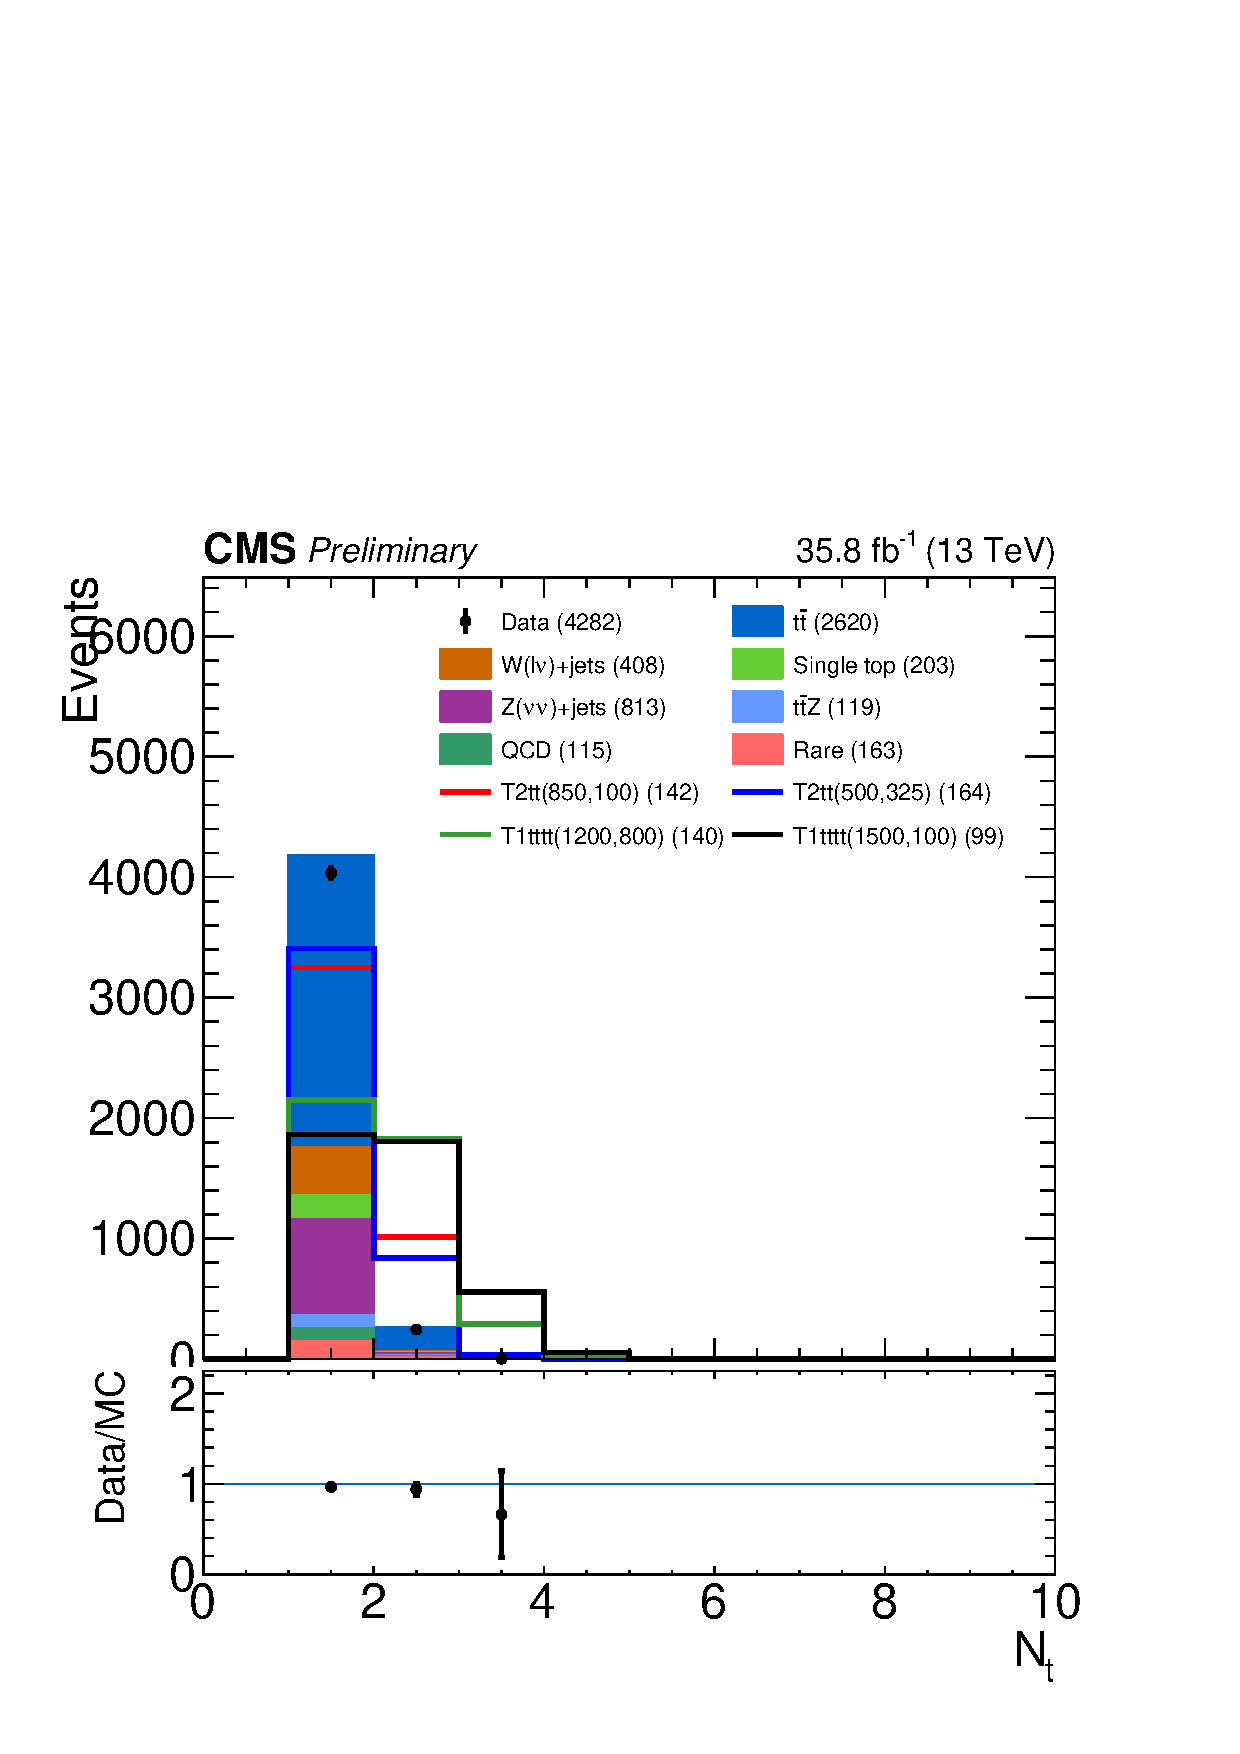
\includegraphics[width=0.45\linewidth]{sections/mc4/EvtSelSBOpt/figures/DataMC_MET_model_NTops_baseline.pdf}
    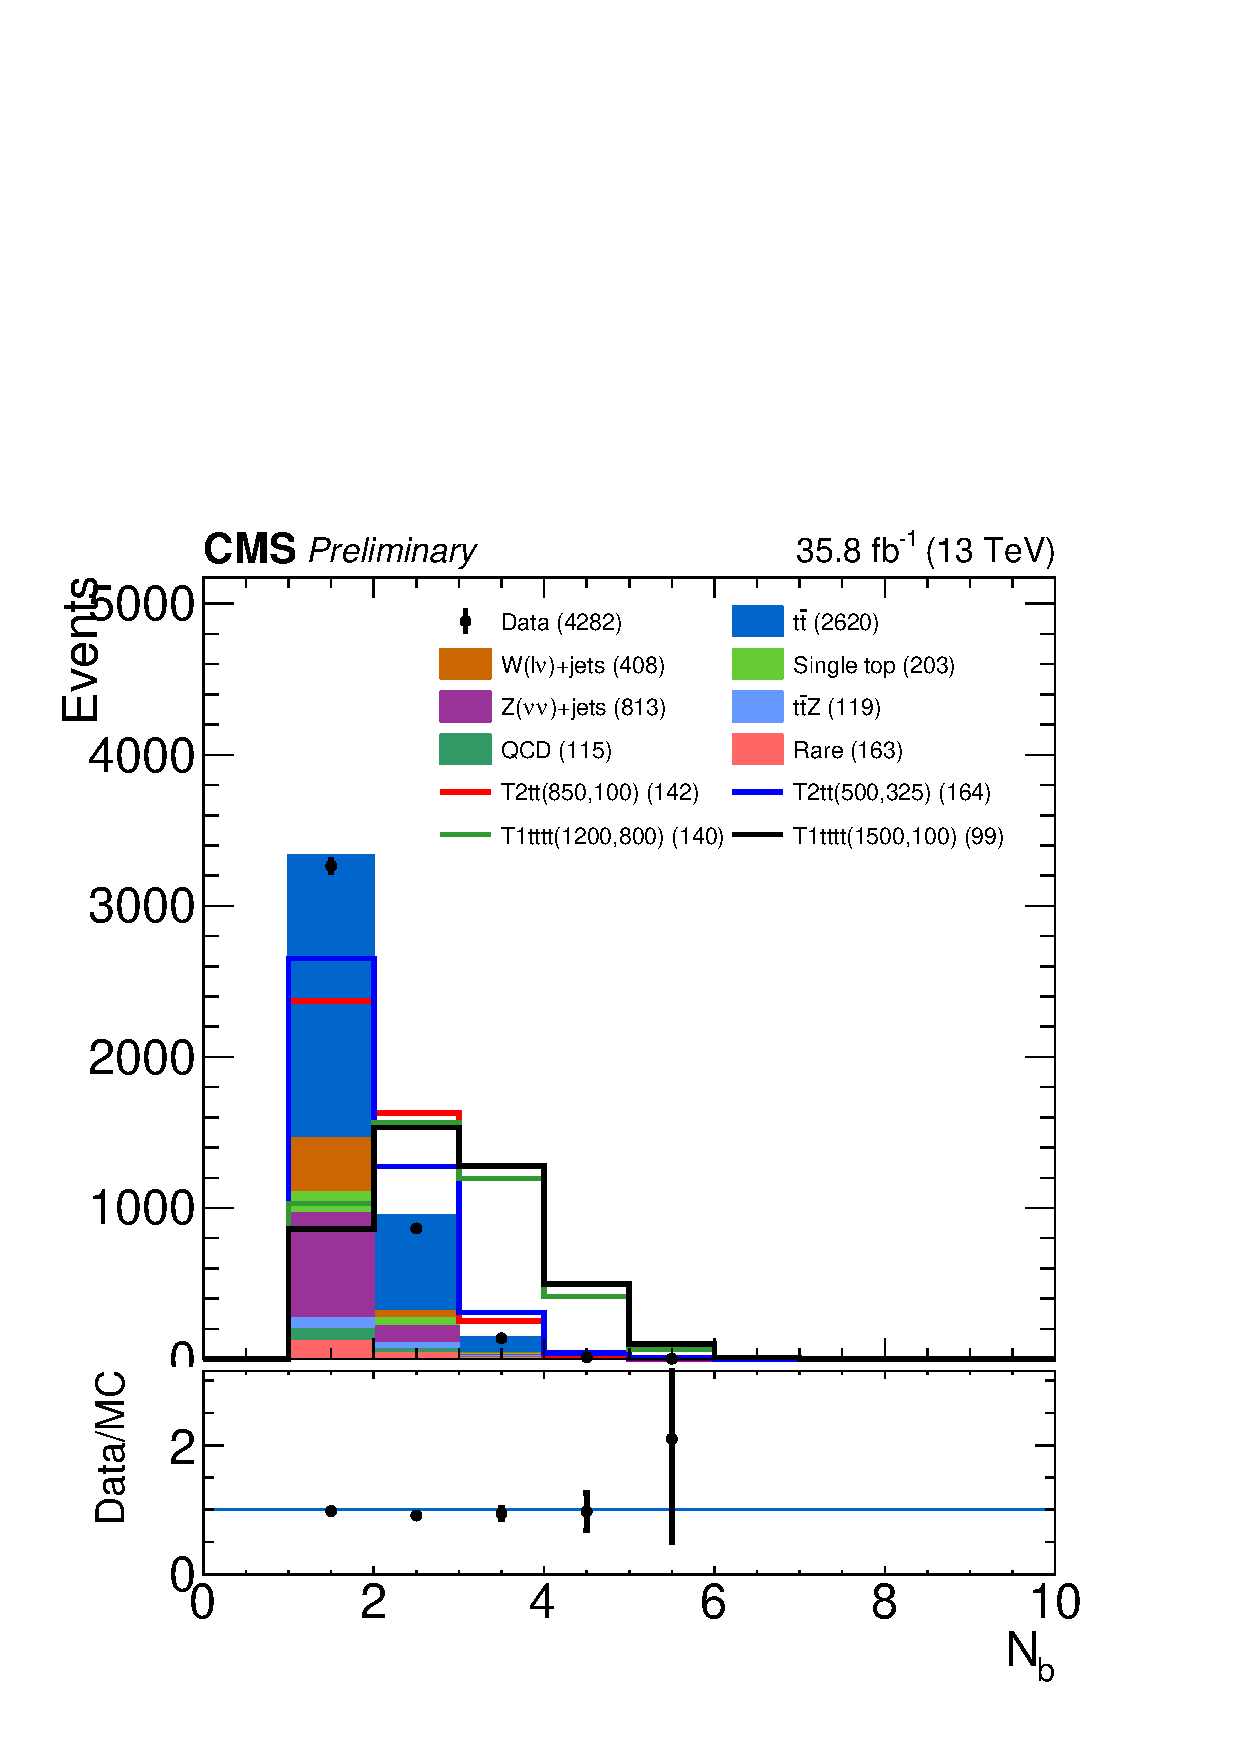
\includegraphics[width=0.45\linewidth]{sections/mc4/EvtSelSBOpt/figures/DataMC_MET_model_NBJEts_baseline.pdf}\\
    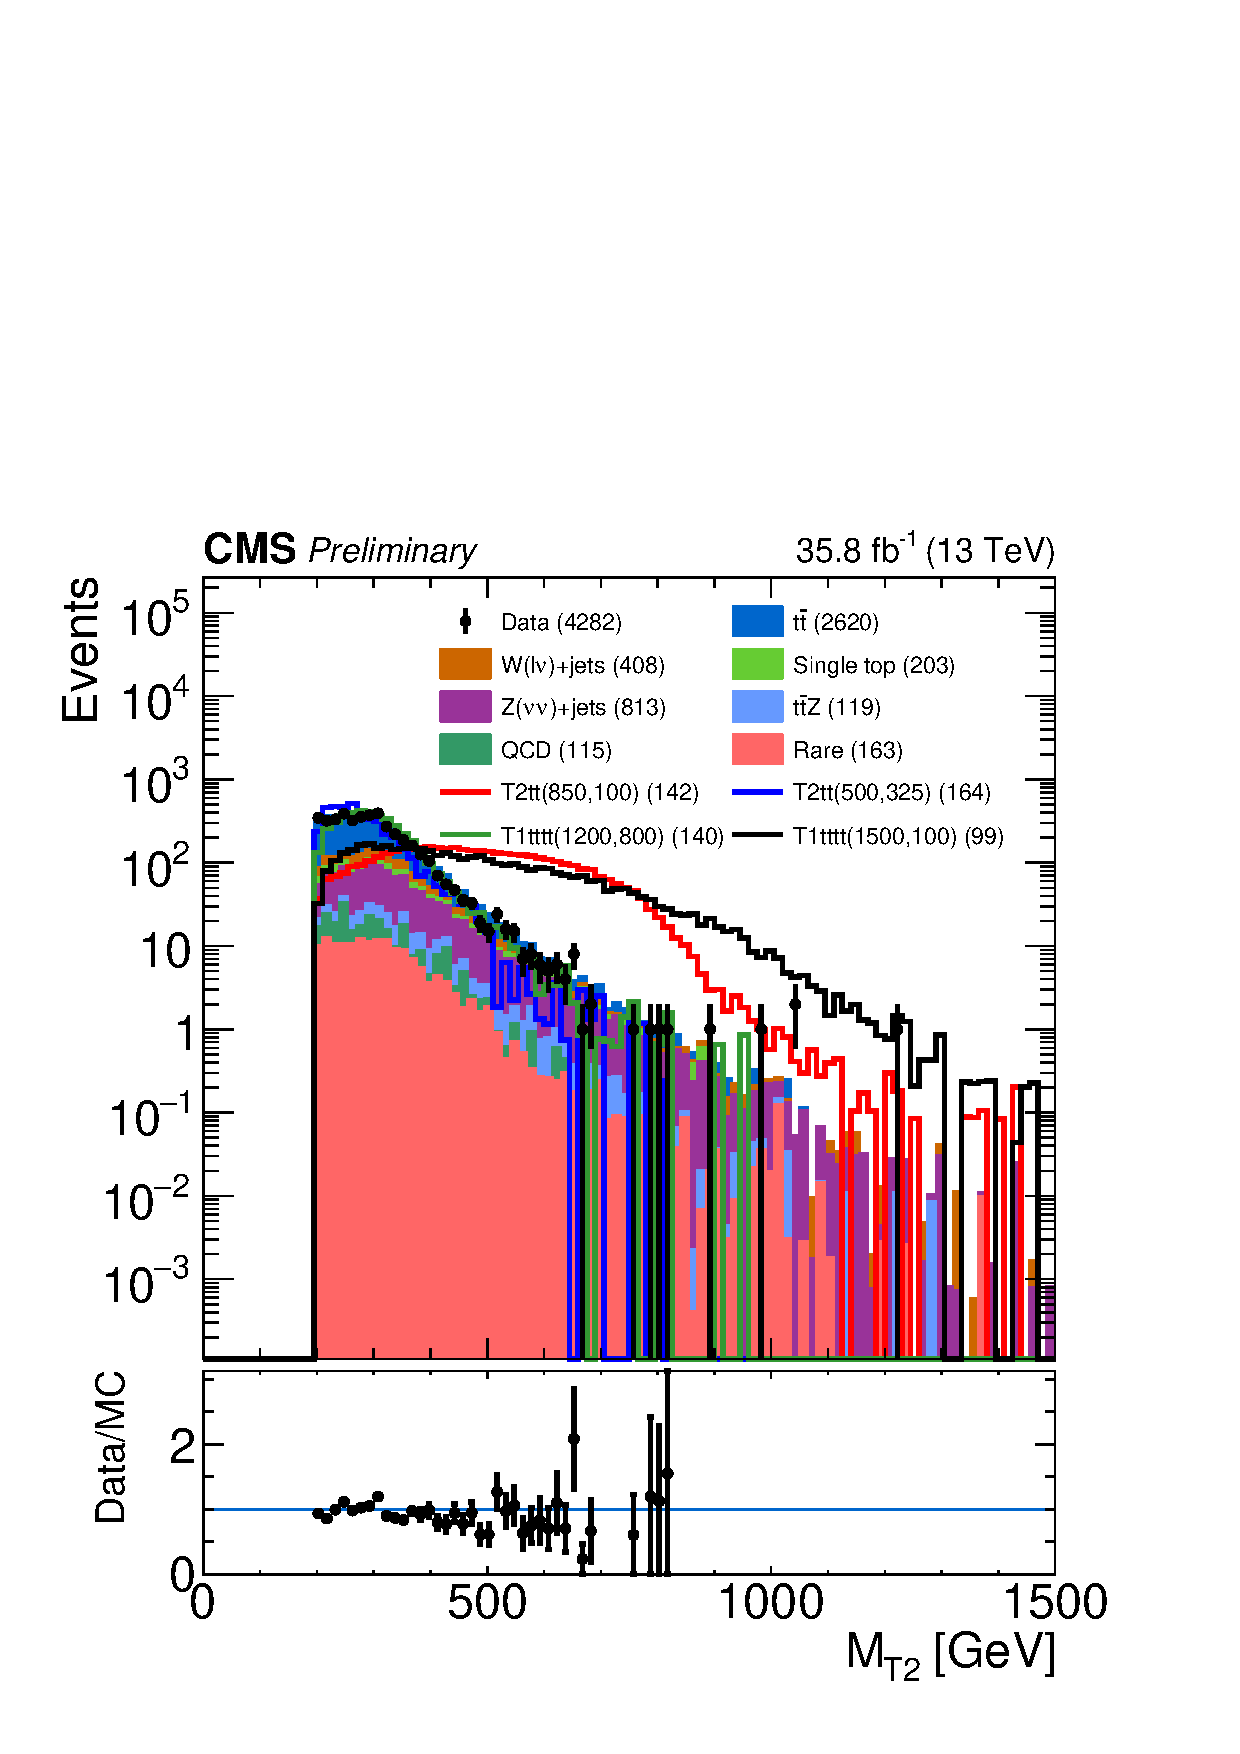
\includegraphics[width=0.45\linewidth]{sections/mc4/EvtSelSBOpt/figures/DataMC_MET_model_MT2_baseline.pdf}
    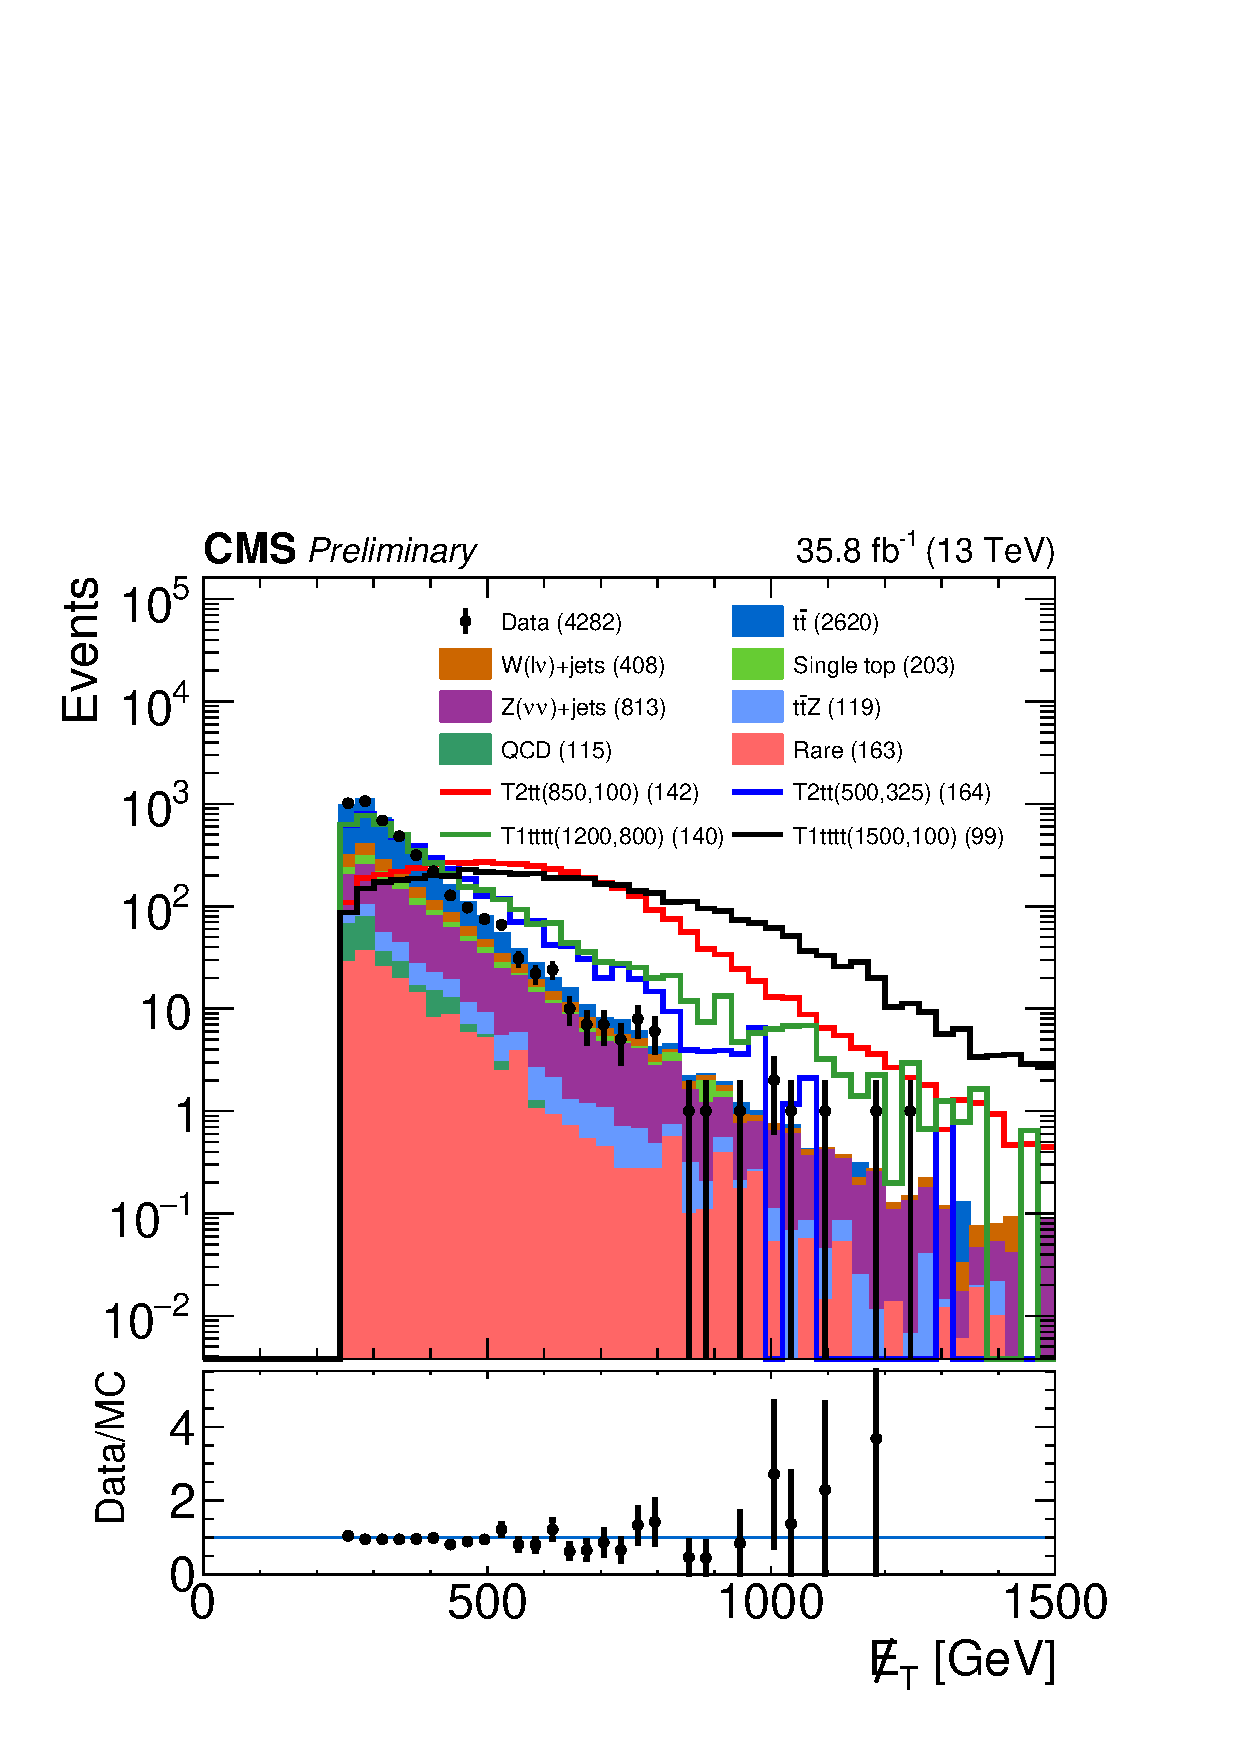
\includegraphics[width=0.45\linewidth]{sections/mc4/EvtSelSBOpt/figures/DataMC_MET_model_met_baseline.pdf}
    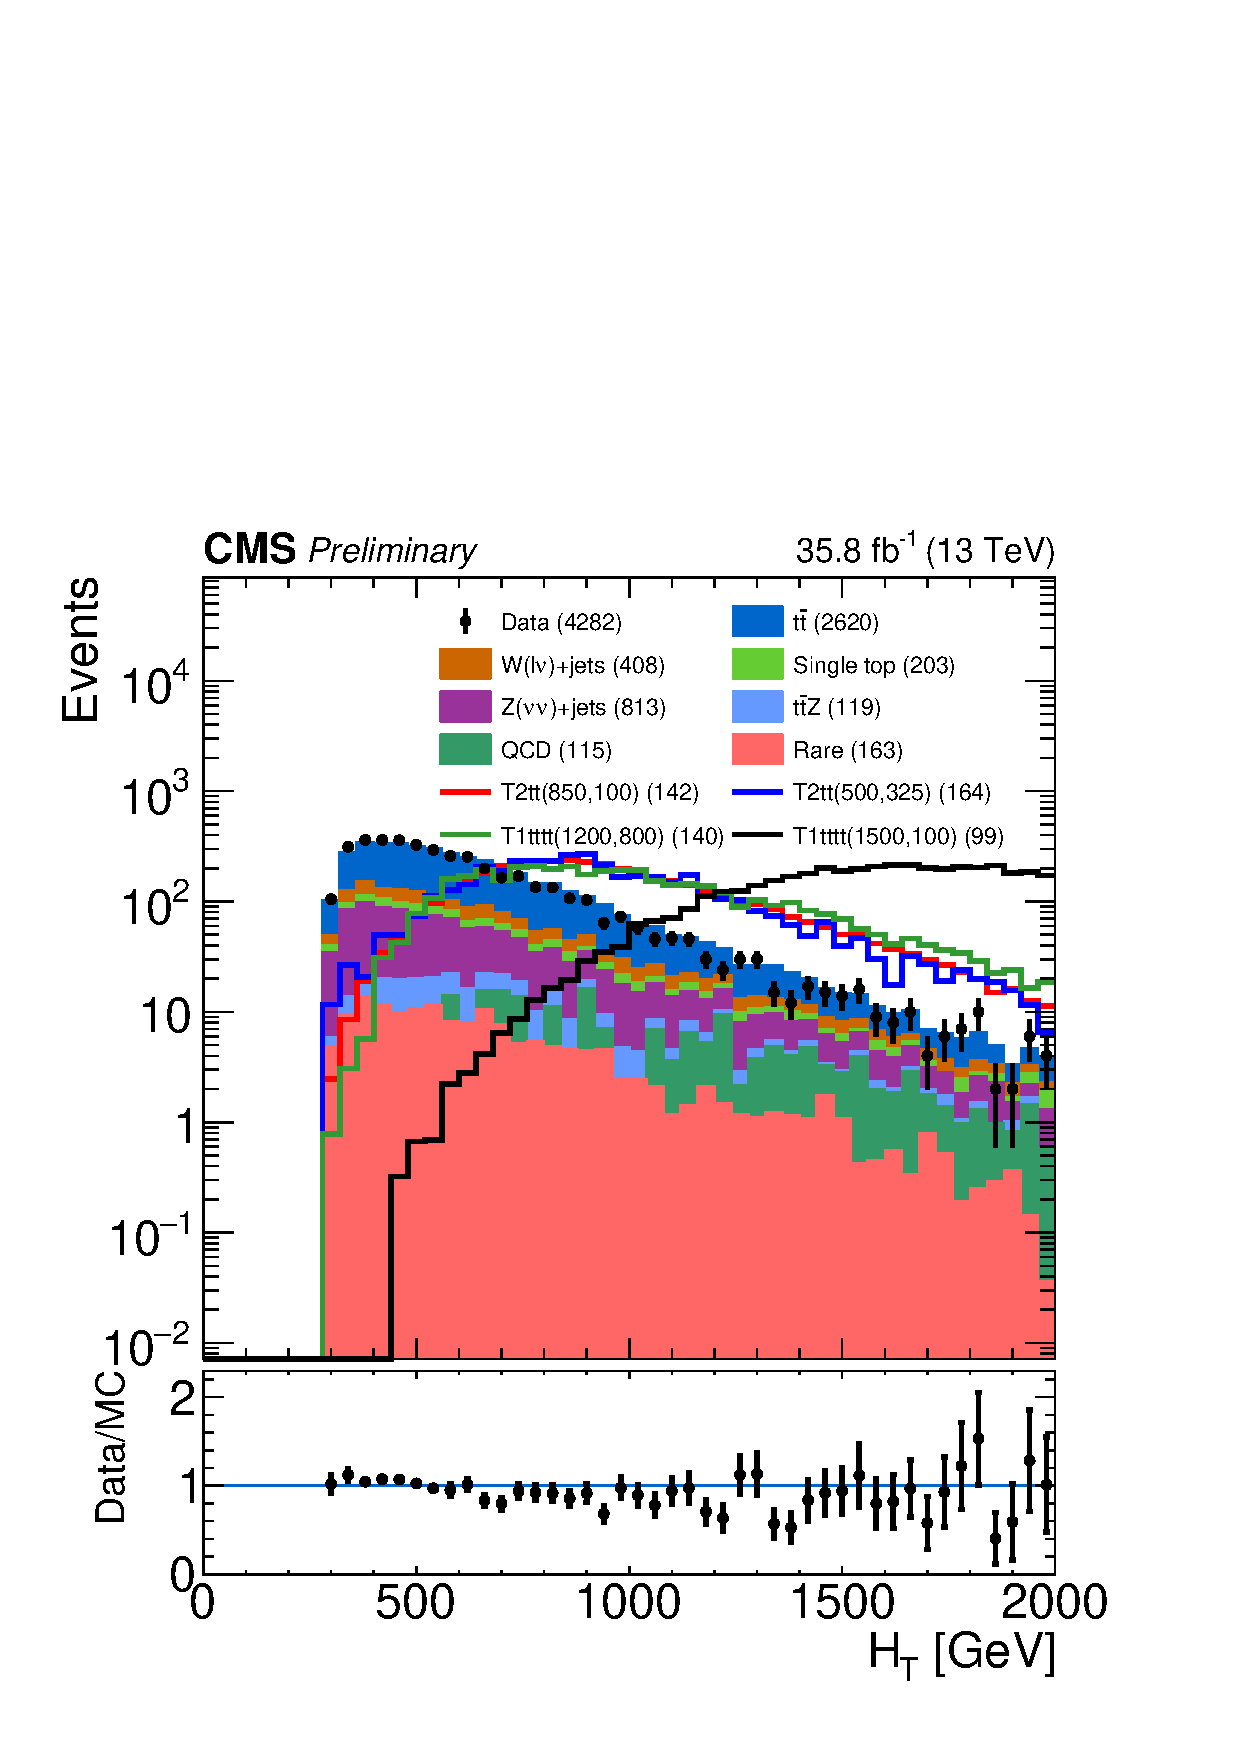
\includegraphics[width=0.45\linewidth]{sections/mc4/EvtSelSBOpt/figures/DataMC_MET_model_ht_baseline.pdf}\\
    \caption{Comparison of the distributions between total SM backgrounds from simulation and several signal points for \ntops, \nbjets, \MET and \MTTwo clock-wise with \HT at the bottom. Total SM backgrounds and signals are scaled to same data yield for a shape comparison. The yeilds for the Data and the SM backgrounds are in the legend.  The scale is included in the legend for the signal points. }
    \label{fig:compSBvars}
  \end{center}
\end{figure}

%Fig.~\ref{fig:compMT2vsMET} shows the 2D distributions of \MTTwo versus \MET for the major \ttbar background and two signals, i.e., T2tt(850, 100) and T2tt(500, 325). We can clearly see the shapes are different between the \ttbar background and the high stop mass signal point. For the low stop mass point, the correlation between \MTTwo and \MET is not as strong as the high mass point, however difference can still be seen between this signal and the \ttbar background.

%\begin{figure}[h]
%  \begin{center}
%    \includegraphics[width=0.32\linewidth]{}%eventSelection/figures/comb_TTbar_MT2_vs_met_baseline.pdf}
%    \includegraphics[width=0.32\linewidth]{}%eventSelection/figures/comb_Signal_T2tt_mStop850_mLSP100_MT2_vs_met_baseline.pdf}
%    \includegraphics[width=0.32\linewidth]{}%eventSelection/figures/comb_Signal_T2tt_mStop500_mLSP325_MT2_vs_met_baseline.pdf}
%    \caption{ 2D distributions of \MTTwo versus \MET for the major \ttbar background and two signal points, i.e., T2tt(850, 100) in the middle and T2tt(500, 325) in the right, after the baseline cuts. }
%    \label{fig:compMT2vsMET}
%  \end{center}
%\end{figure}

The search bins defined after baseline cuts (in total 84 bins) are illustrated in Fig.~\ref{fig:SBXX}. An improvement we make is switching from the \MTTwo variable to \HT variable for search bins where $\nbjets>=3$ or $\ntops>=3$ since these bins should be sensitive to the T1tttt signals where the \MTTwo cannot be clearly as defined with more than two reconstructed top quarks or provide the best sensitivity. 
To accommodate with increaing luminosity of 2016 data and improve our search sensitivity, we make harder search bins in
\MET, \HT and \MTTwo dimentions. The optimization was based on significance scan of each of \MET, \MTTwo and \HT dimentions. However
furthur adjustment was done to have reasonable control sample events for major background predictions.
The numbers displayed in the figures are the binning indices which are used throughout the analysis.
The bins with $\ntops>=3$ are important for T1tttt signal but for T2tt we do not use them for limit calculation.

\begin{figure}[h]
  \begin{center}
    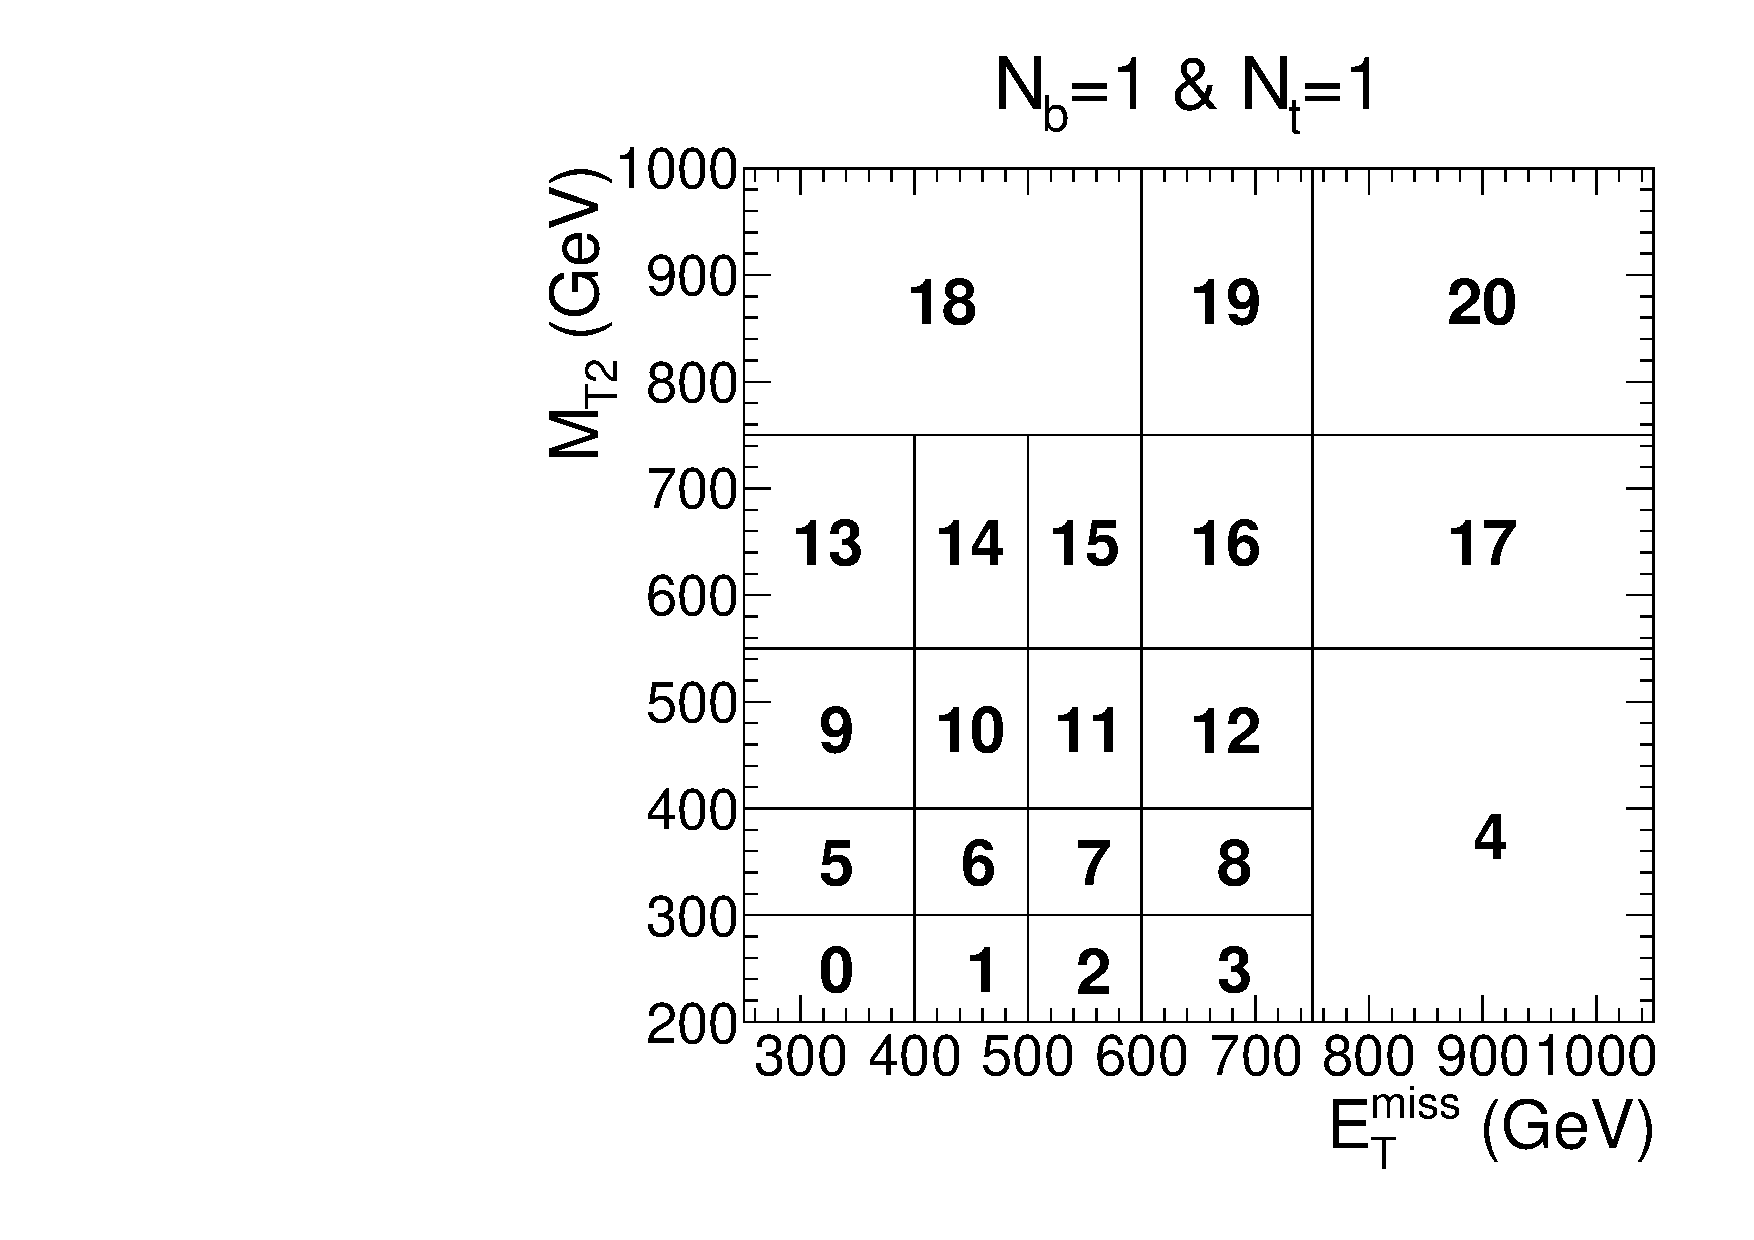
\includegraphics[width=0.30\linewidth]{sections/mc4/EvtSelSBOpt/figures/poly_MT2_vs_met_0.pdf}
    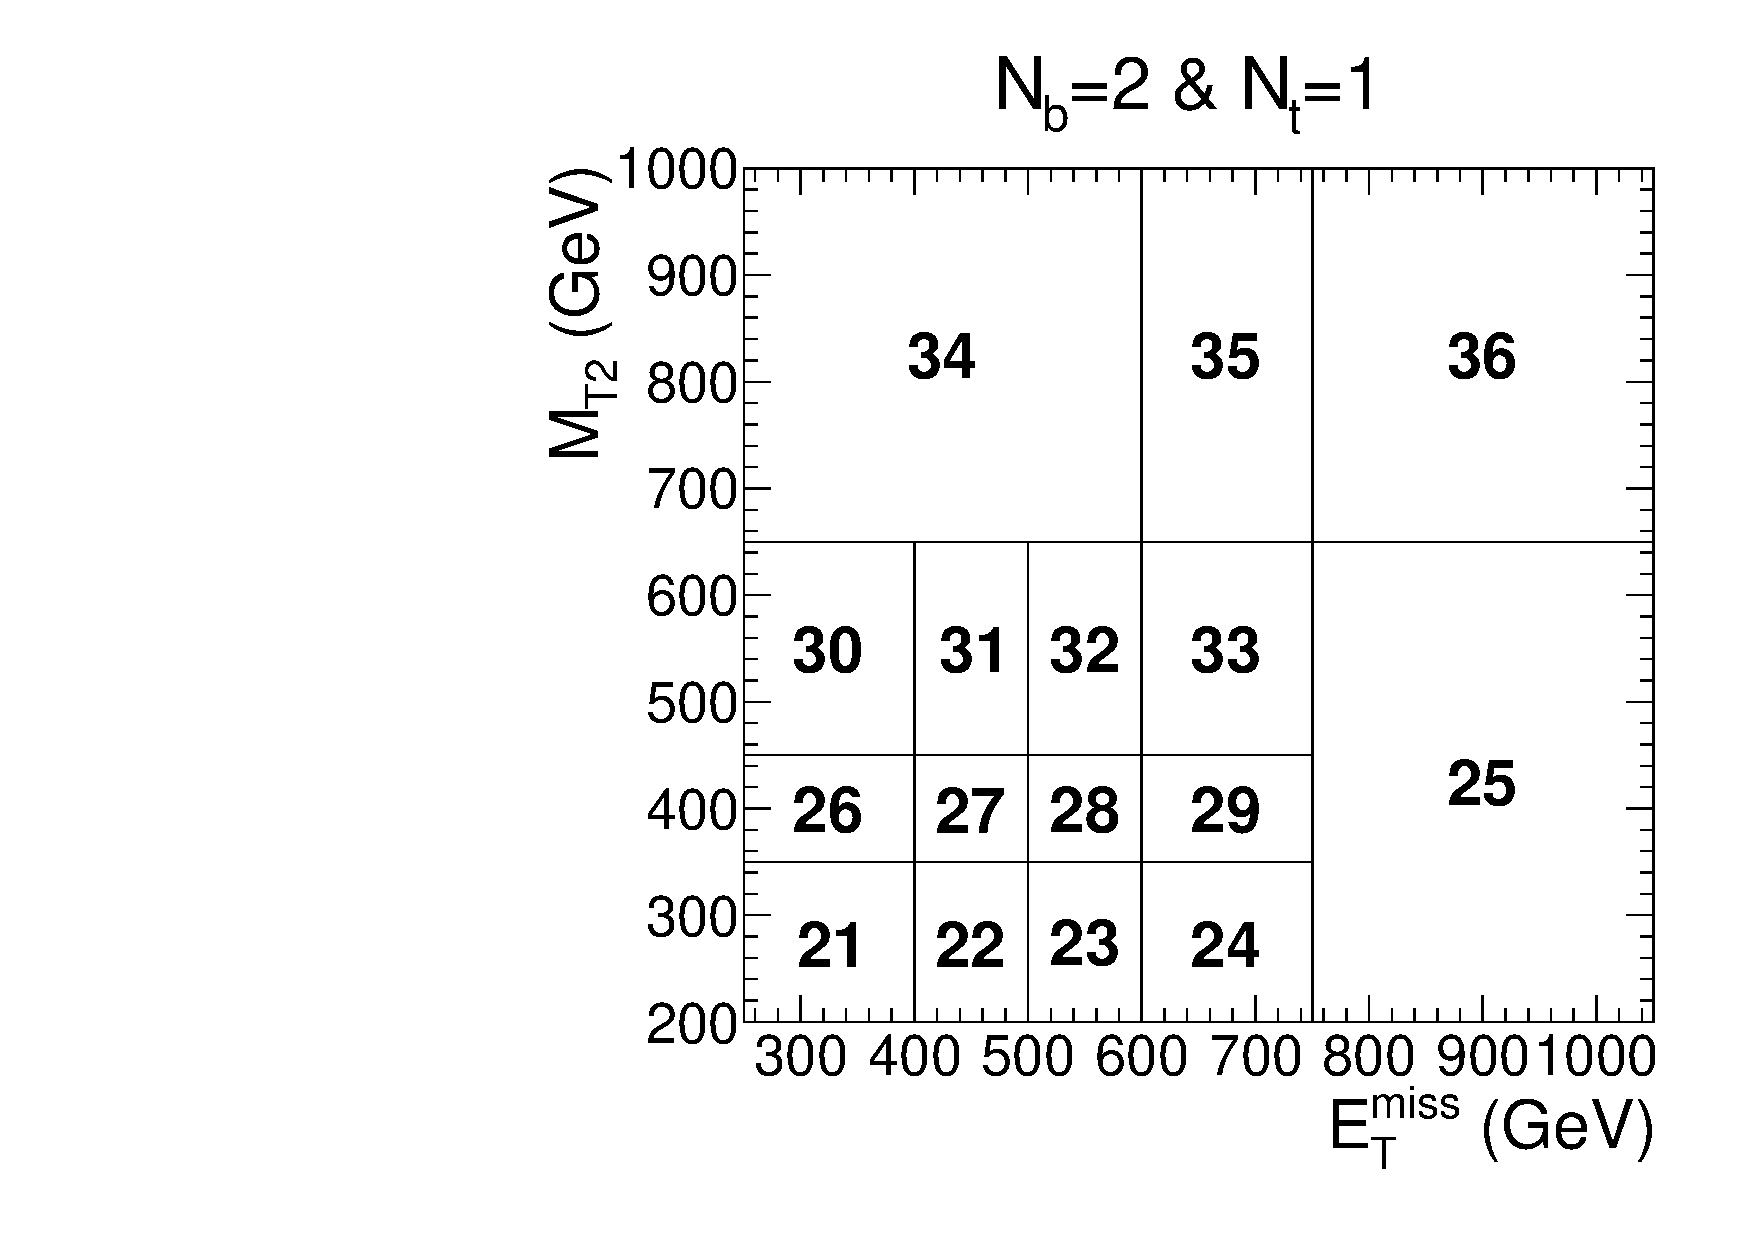
\includegraphics[width=0.30\linewidth]{sections/mc4/EvtSelSBOpt/figures/poly_MT2_vs_met_1.pdf}
    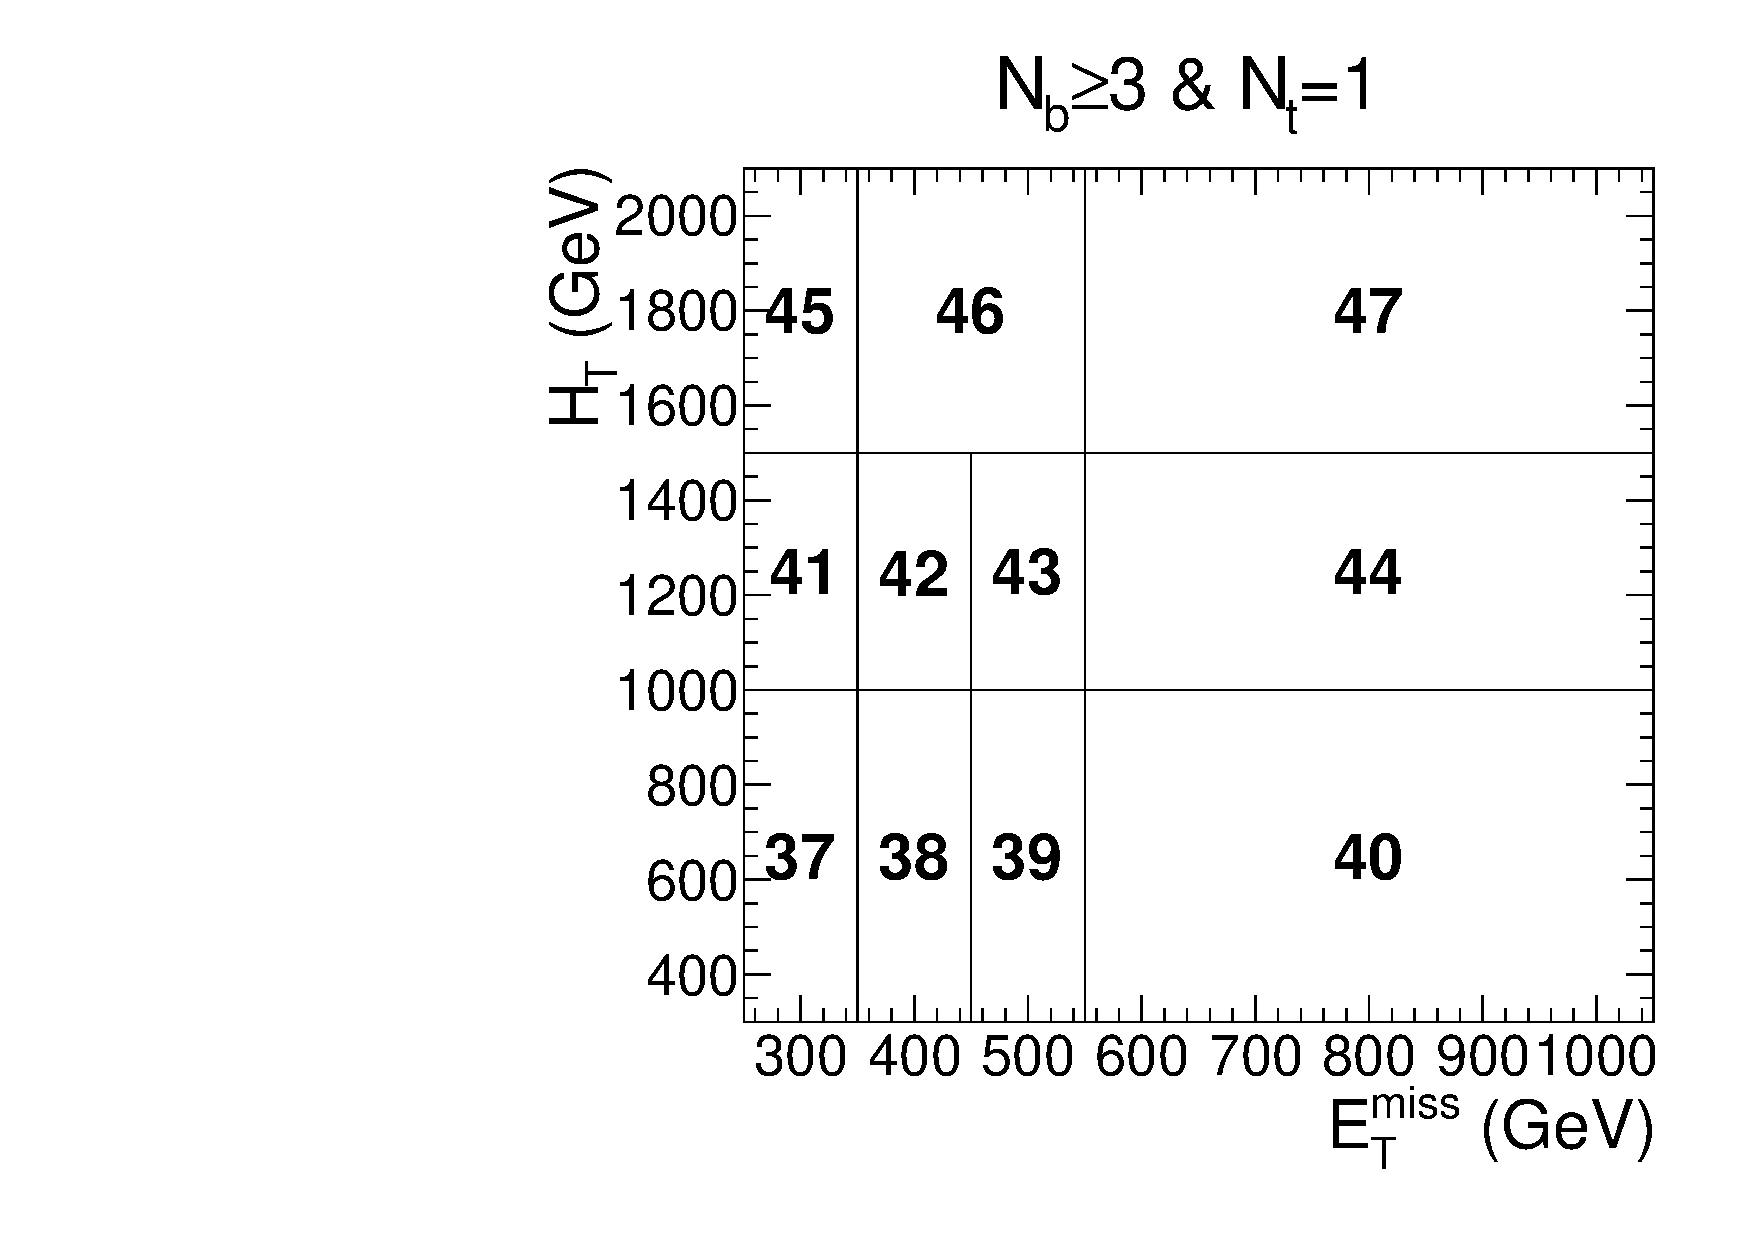
\includegraphics[width=0.30\linewidth]{sections/mc4/EvtSelSBOpt/figures/poly_MT2_vs_met_2.pdf} \\
    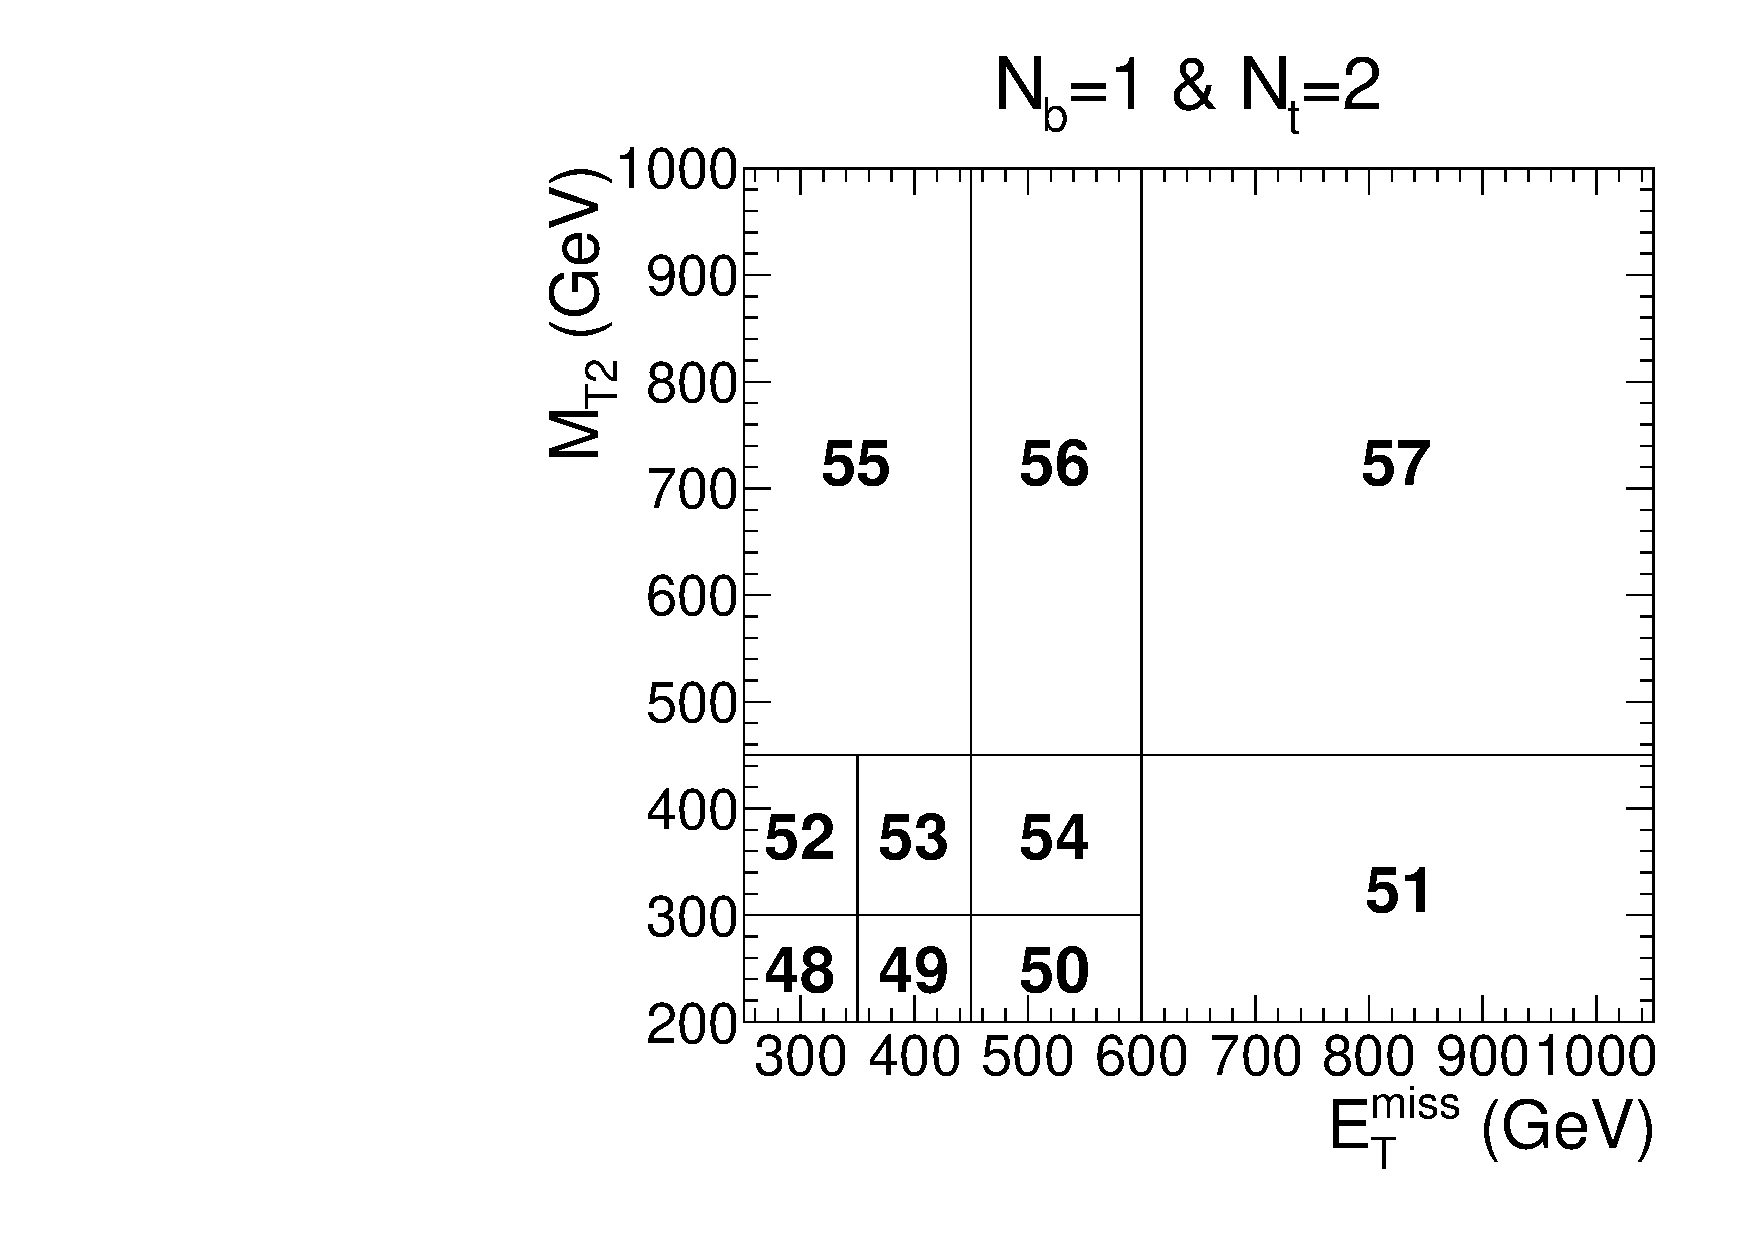
\includegraphics[width=0.30\linewidth]{sections/mc4/EvtSelSBOpt/figures/poly_MT2_vs_met_3.pdf} 
    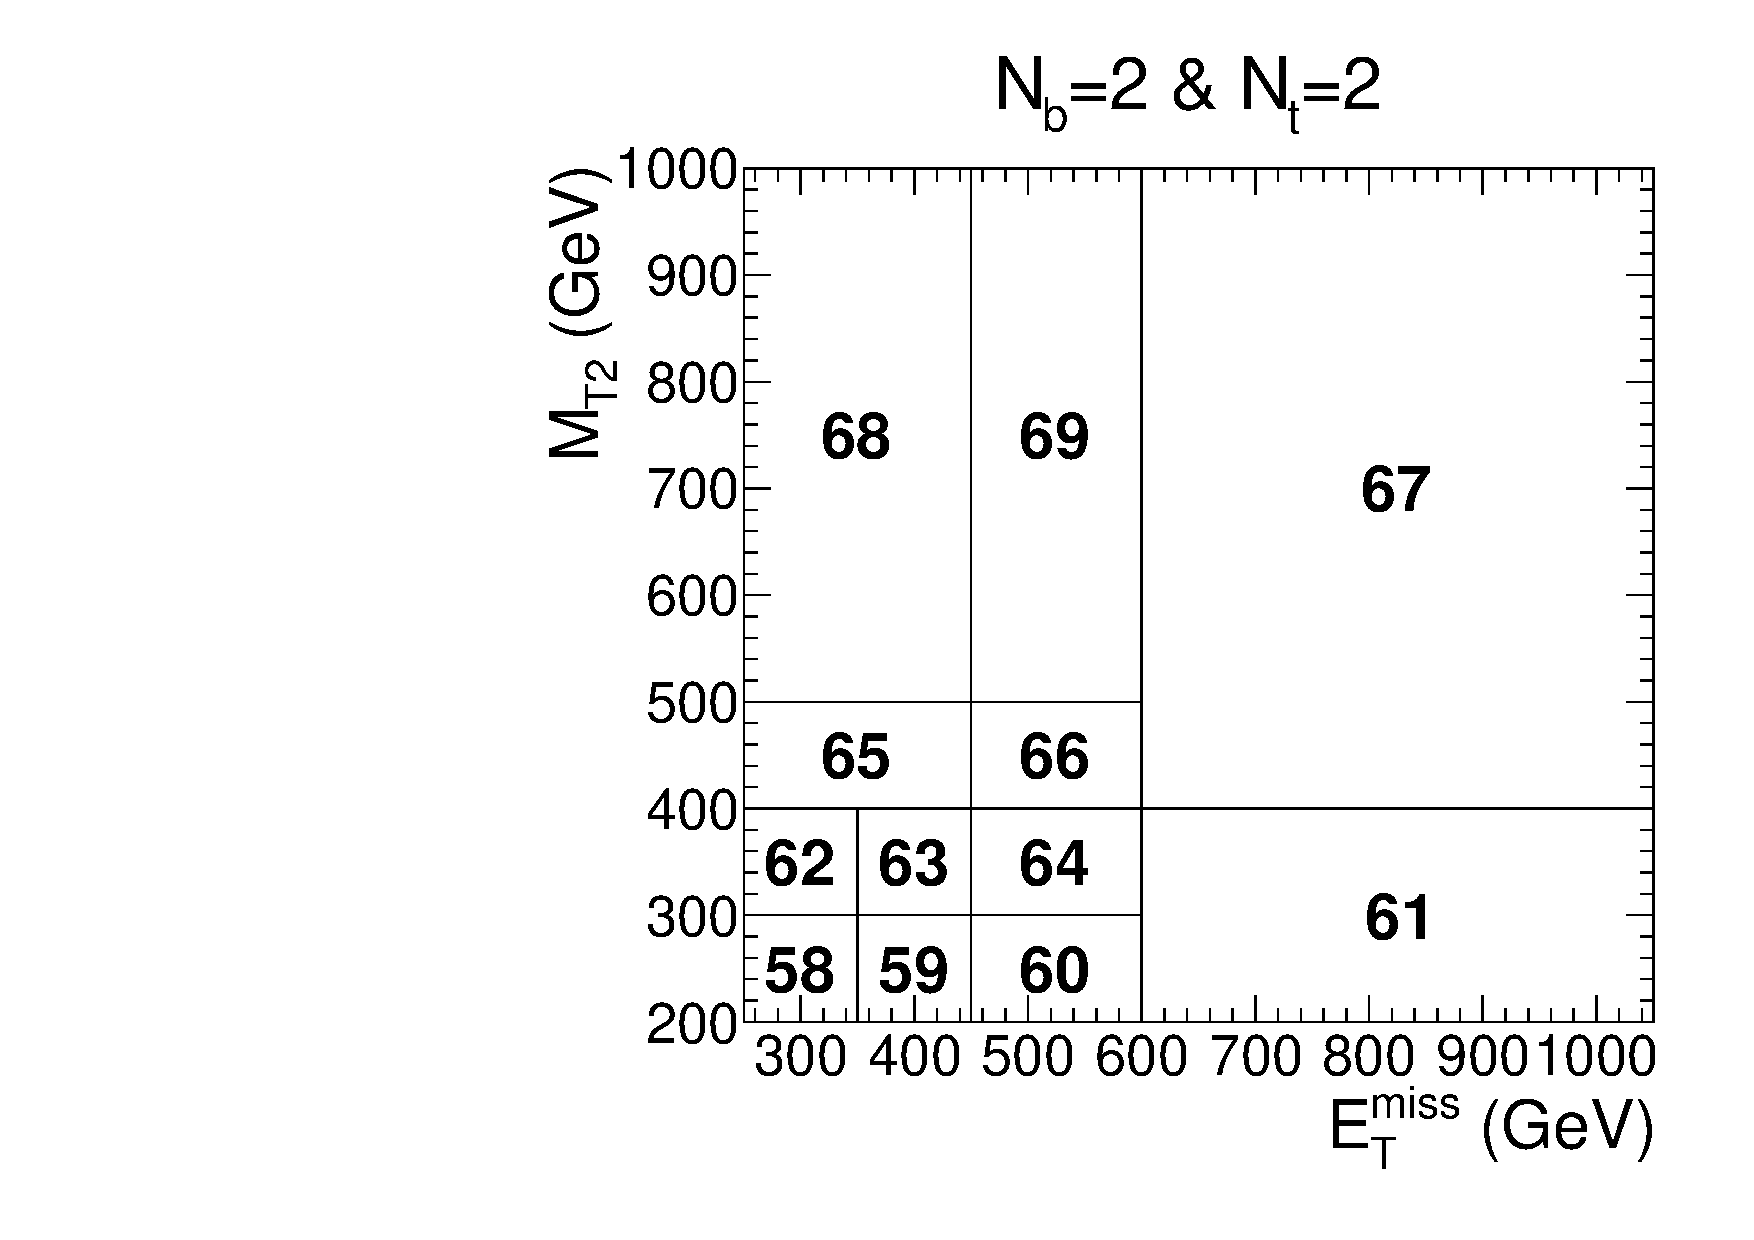
\includegraphics[width=0.30\linewidth]{sections/mc4/EvtSelSBOpt/figures/poly_MT2_vs_met_4.pdf} 
    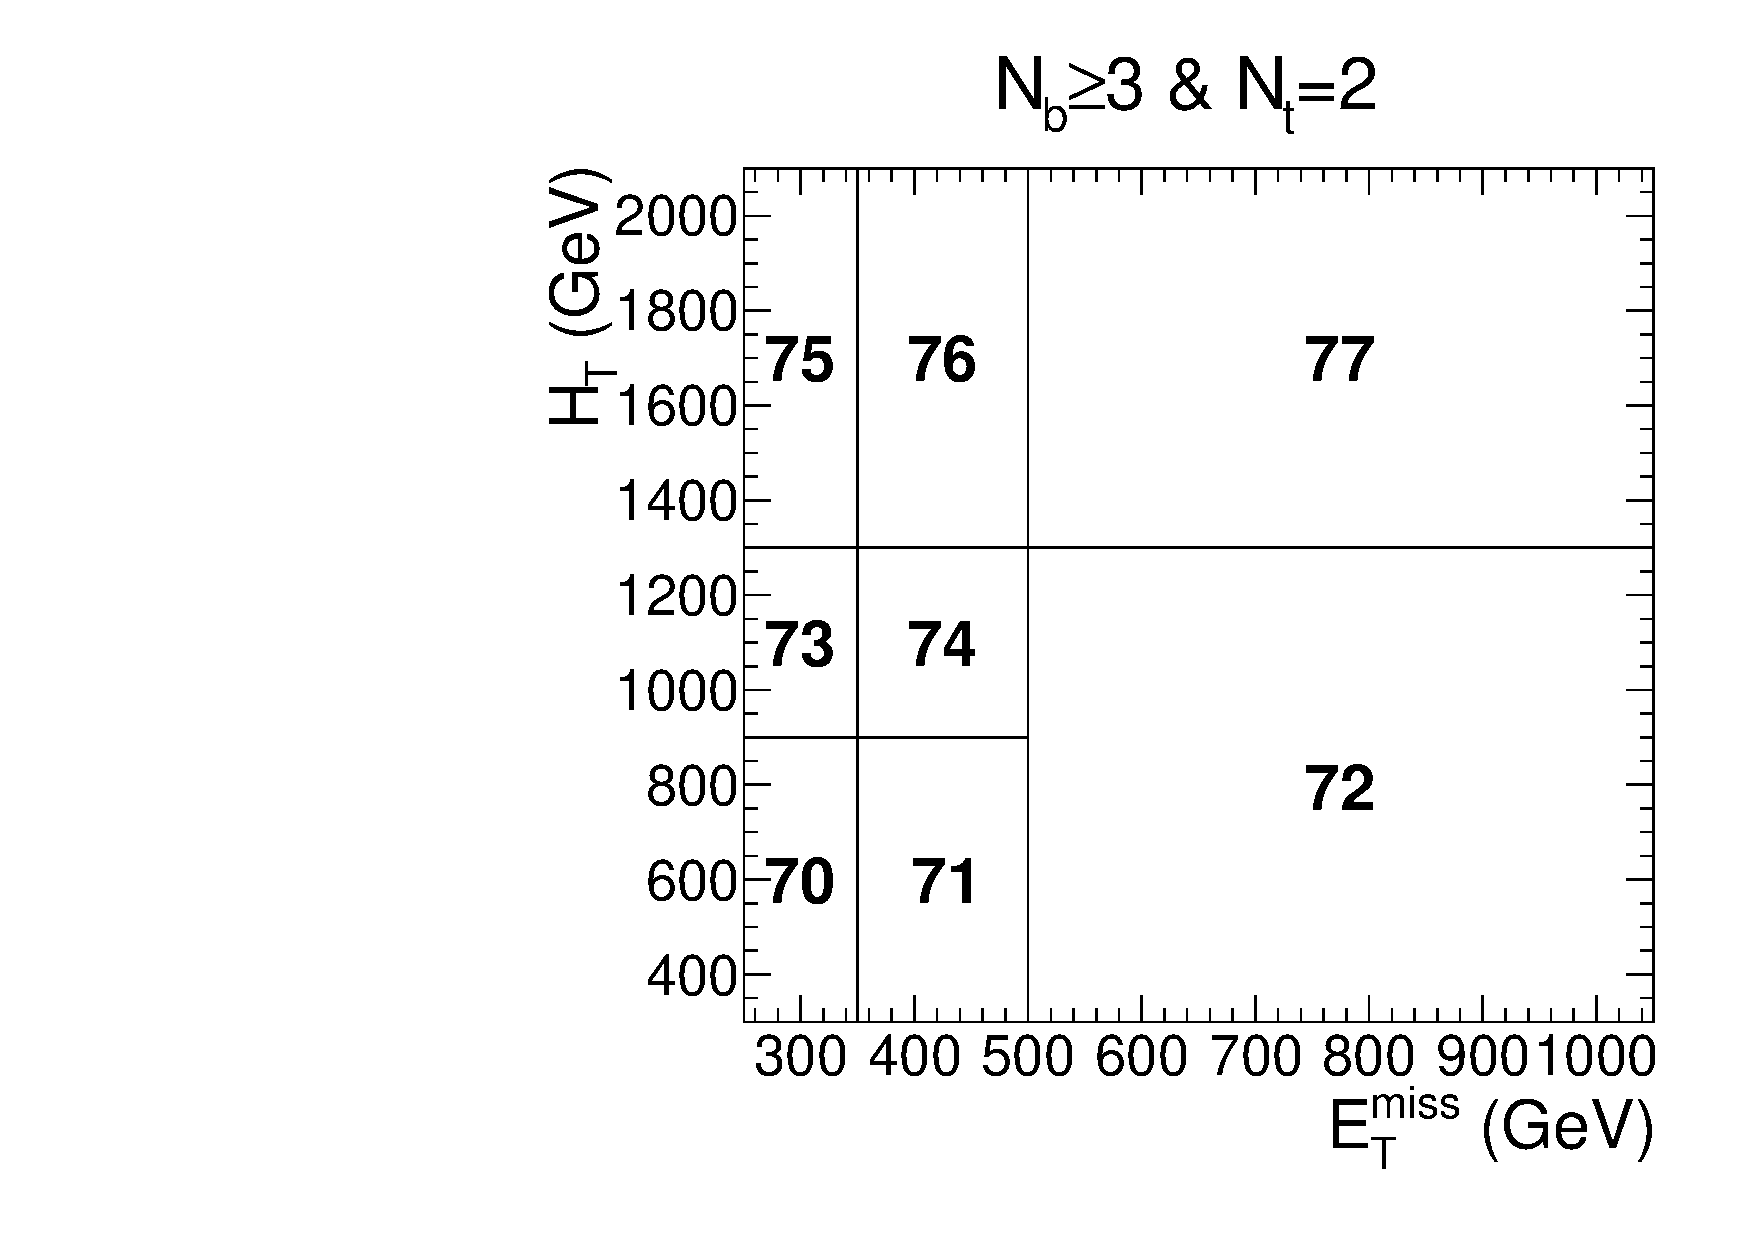
\includegraphics[width=0.30\linewidth]{sections/mc4/EvtSelSBOpt/figures/poly_MT2_vs_met_5.pdf} \\
    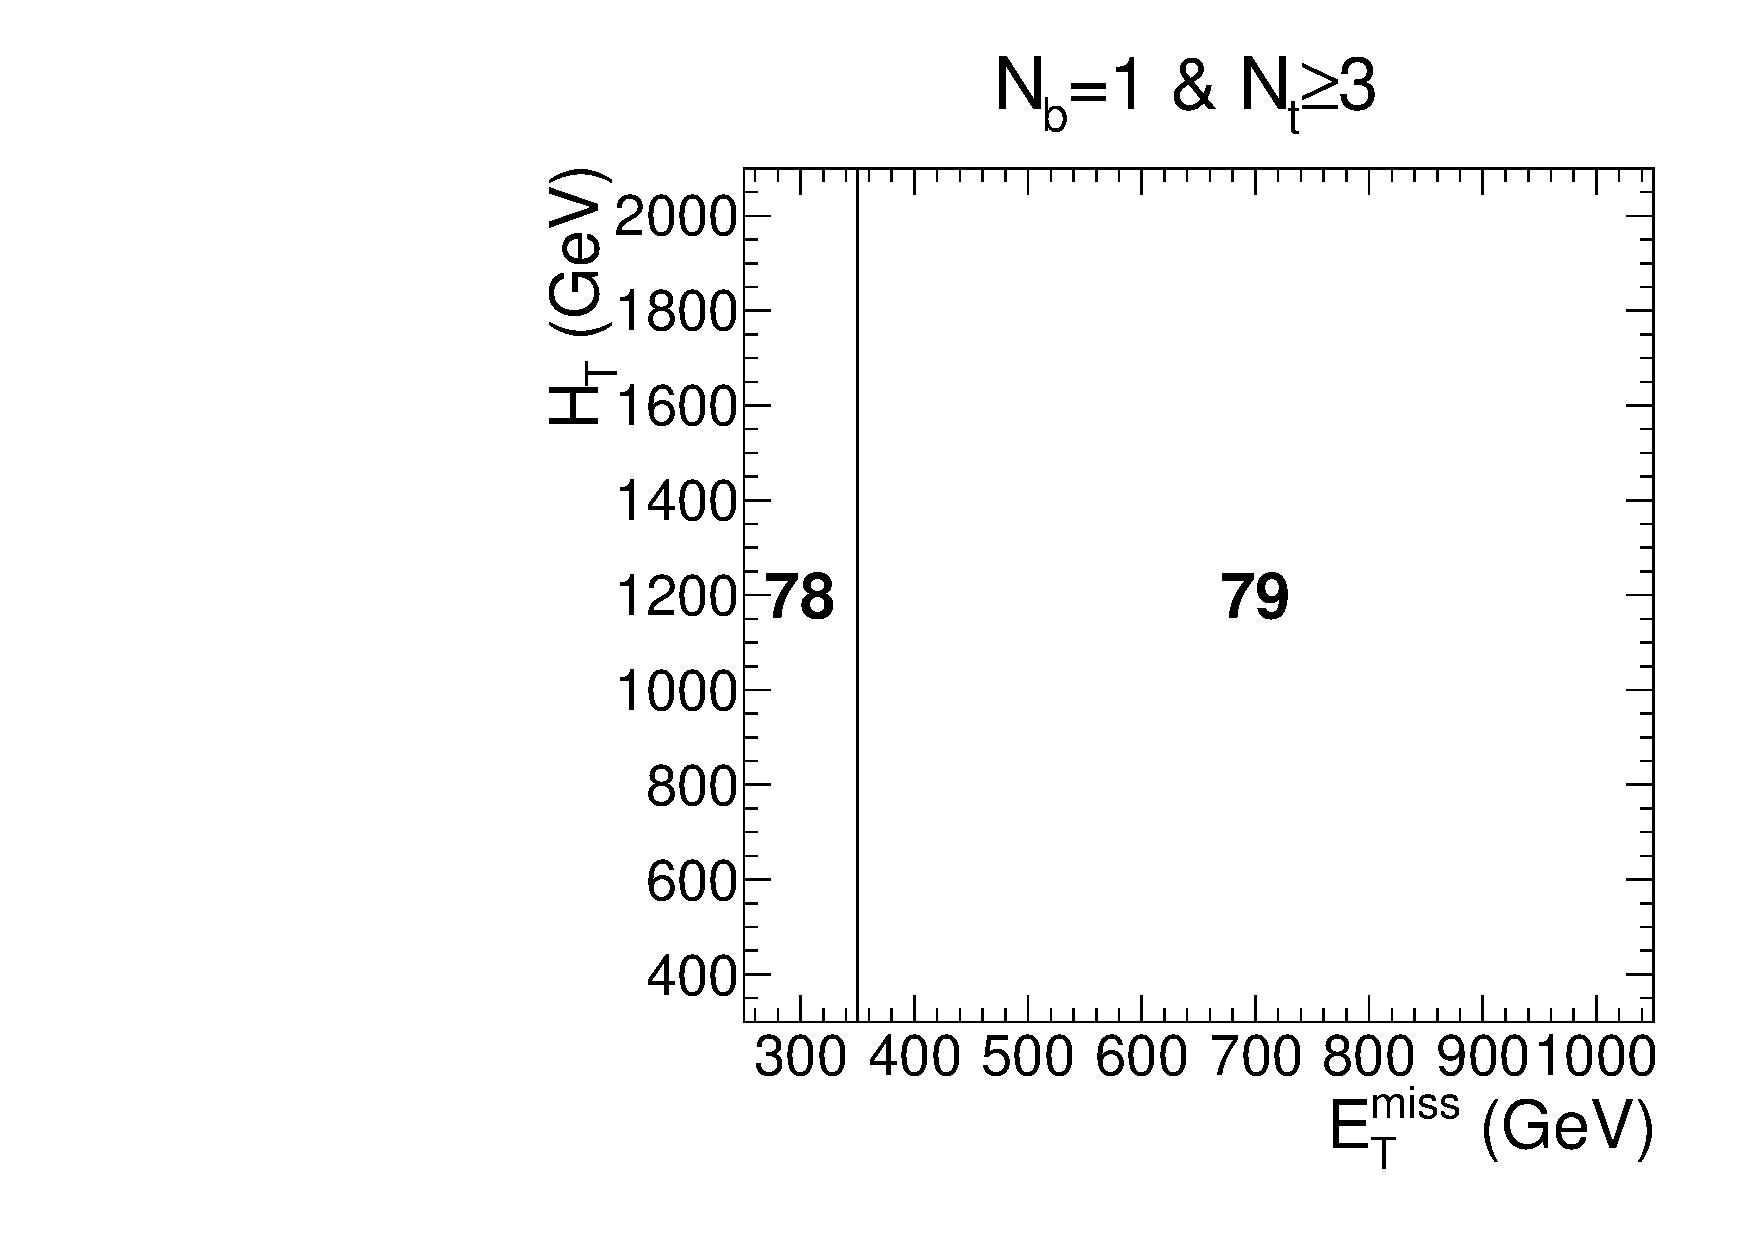
\includegraphics[width=0.30\linewidth]{sections/mc4/EvtSelSBOpt/figures/poly_MT2_vs_met_6.pdf} 
    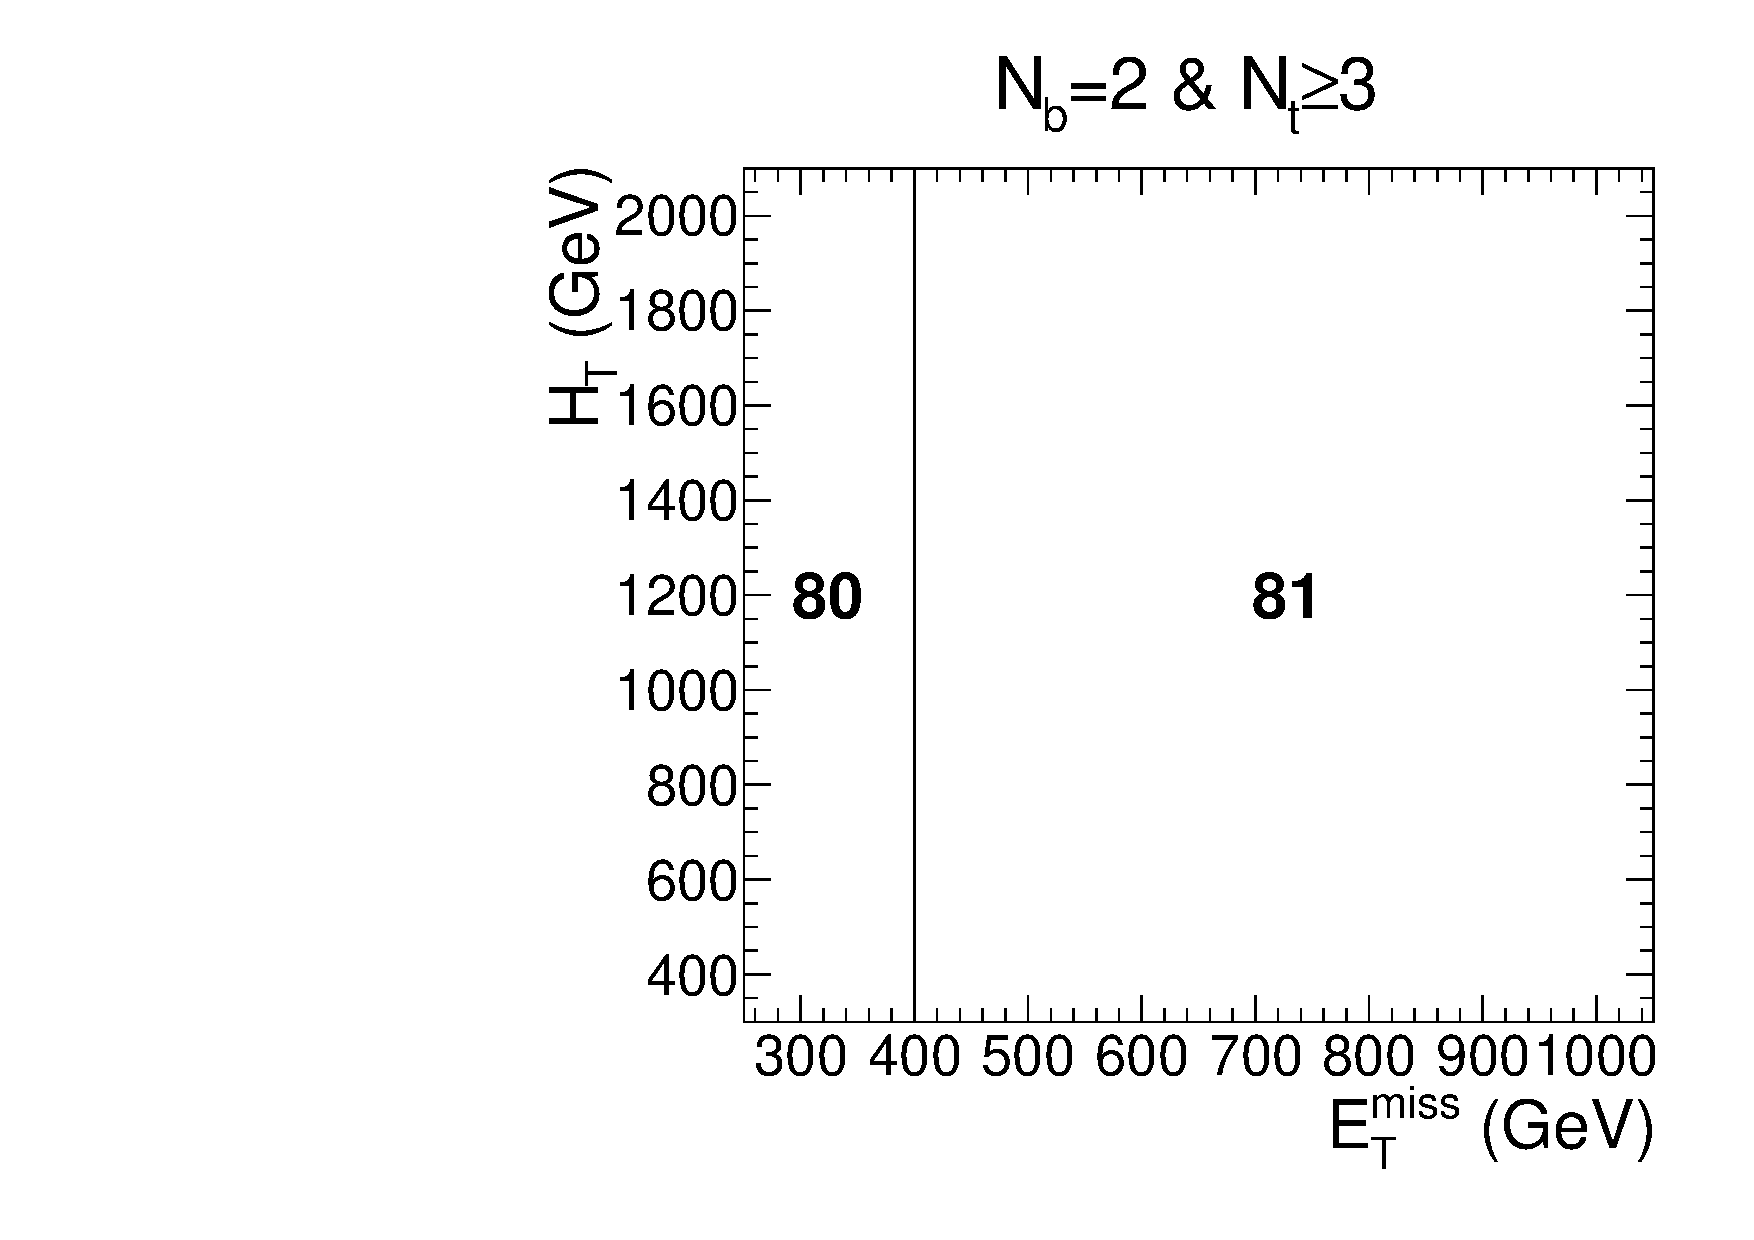
\includegraphics[width=0.30\linewidth]{sections/mc4/EvtSelSBOpt/figures/poly_MT2_vs_met_7.pdf} 
    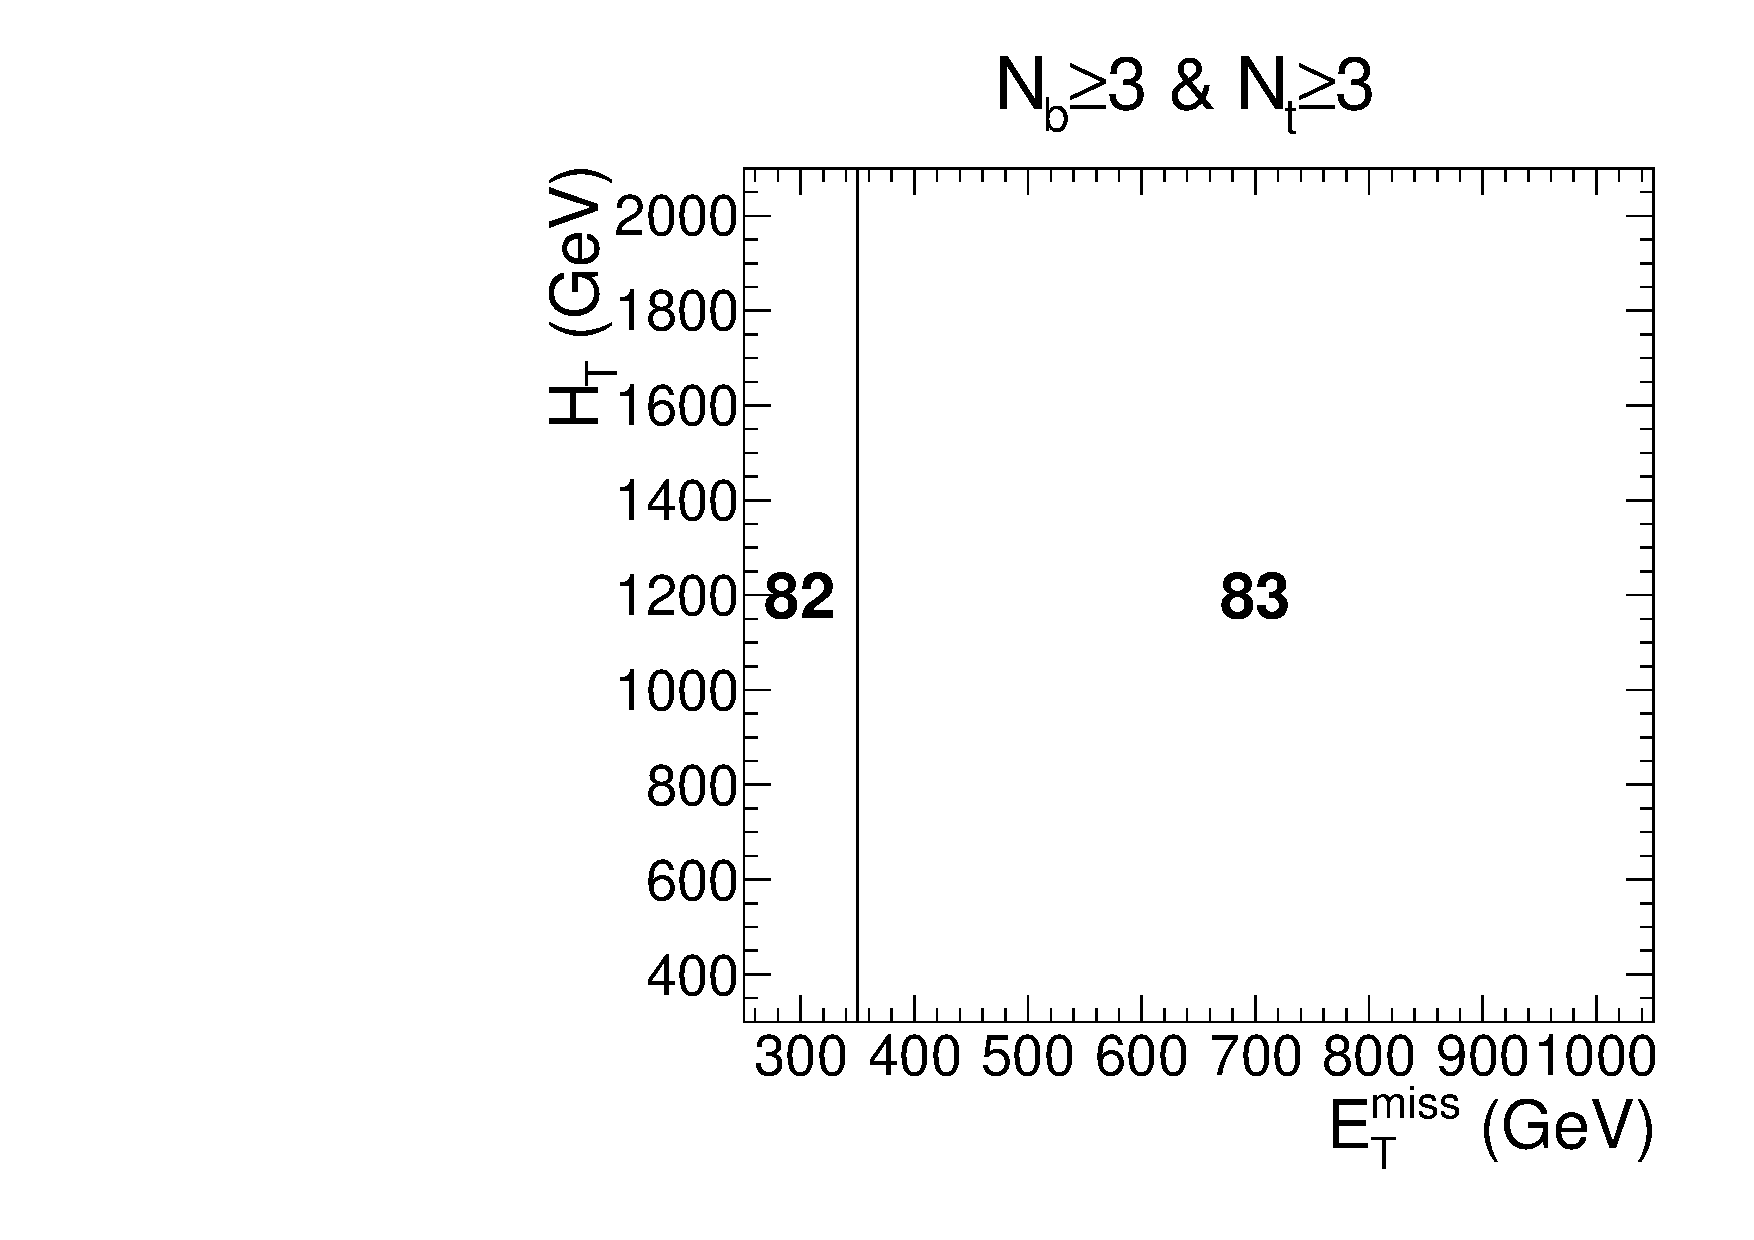
\includegraphics[width=0.30\linewidth]{sections/mc4/EvtSelSBOpt/figures/poly_MT2_vs_met_8.pdf} \\
    \caption{Original search bin definitions after baseline cuts (in total 84 search bins). }
    \label{fig:SBXX}
  \end{center}
\end{figure}

\subsection{MC samples for Background and Signal Studies}
\label{sec:sm-mc}

The analysis uses a set of Monte Carlo samples for background estimation method
development and predictions as well as SUSY signal samples for interpretation
of the results in the light of a number of simplified models. All the
background samples are generated with the Geant4-based CMS simulation 
application while all the signal samples for limit setting are generated
using the Fast Simulation application.

\paragraph{Standard Model Samples}

Monte Carlo samples of SM processes reconstructed with CMSSW release 8.0 
(Summer16) are used throughout this analysis note.
A complete list of these samples is shown in Tab.~\ref{tab:MCsamples}. 
The cross sections listed come from calculations performed at the 
next-to-next-to-leading-order (NNLO) unless otherwise noted.
All samples use the ``Moriond17" pileup scenario, which simulates a pileup 
distribution with an average of 25 interactions per bunch crossing and a 
25~ns interval between bunches.

% This table is out-dated, if needed, can copy the table from the MT2 AN2016_460
\begin{table}[hp]
\centering
\caption{Standard model Monte Carlo samples used in the analysis.}
\label{tab:MCsamples}
{\footnotesize
\begin{tabular}{lccc}
\hline \hline
Dataset & $\sigma$ (pb) & $\int$ (fb$^{-1}$) \\
\hline
\multicolumn{3}{c}{QCD MC samples (LO)} \\ \hline
QCD\_HT100to200\_TuneCUETP8M1\_13TeV-madgraphMLM-pythia8 & 27540000 & 0.01\\
QCD\_HT200to300\_TuneCUETP8M1\_13TeV-madgraphMLM-pythia8 & 1735000 & 0.01\\
QCD\_HT300to500\_TuneCUETP8M1\_13TeV-madgraphMLM-pythia8 & 366800 & 0.05\\
QCD\_HT500to700\_TuneCUETP8M1\_13TeV-madgraphMLM-pythia8 & 29370 & 0.67\\
QCD\_HT700to1000\_TuneCUETP8M1\_13TeV-madgraphMLM-pythia8 & 6524 & 2.30\\
QCD\_HT1000to1500\_TuneCUETP8M1\_13TeV-madgraphMLM-pythia8 & 1064 & 4.67\\
QCD\_HT1500to2000\_TuneCUETP8M1\_13TeV-madgraphMLM-pythia8 & 121.5 & 31.67\\
QCD\_HT2000toInf\_TuneCUETP8M1\_13TeV-madgraphMLM-pythia8 & 25.42 & 77.17\\
\hline
\multicolumn{3}{c}{SM \ttbar MC samples} \\ \hline
%TTJets\_TuneCUETP8M1\_13TeV-madgraphMLM-pythia8 & 816.0 & 13.90\\
TTJets\_SingleLeptFromT\_TuneCUETP8M1\_13TeV-madgraphMLM-pythia8 & 179.3 & 324.6\\
TTJets\_SingleLeptFromTbar\_TuneCUETP8M1\_13TeV-madgraphMLM-pythia8 & 179.3 & 335.7\\
TTJets\_DiLept\_TuneCUETP8M1\_13TeV-madgraphMLM-pythia8 & 86.66 & 351.2\\
TTJets\_HT-600to800\_TuneCUETP8M1\_13TeV-madgraphMLM-pythia8 & 2.615 & 1898\\
TTJets\_HT-800to1200\_TuneCUETP8M1\_13TeV-madgraphMLM-pythia8 & 1.077 & 3198\\
TTJets\_HT-1200to2500\_TuneCUETP8M1\_13TeV-madgraphMLM-pythia8 & 0.195 & 5063\\
TTJets\_HT-2500toInf\_TuneCUETP8M1\_13TeV-madgraphMLM-pythia8 & 0.002 & 218575\\
\hline
\multicolumn{3}{c}{SM \wlnu MC samples} \\ \hline
WJetsToLNu\_HT-100To200\_TuneCUETP8M1\_13TeV-madgraphMLM-pythia8 & 1635 & 6.20\\
WJetsToLNu\_HT-200To400\_TuneCUETP8M1\_13TeV-madgraphMLM-pythia8 & 437.0 & 11.97\\
WJetsToLNu\_HT-400To600\_TuneCUETP8M1\_13TeV-madgraphMLM-pythia8 & 59.50 & 31.96\\
WJetsToLNu\_HT-600ToInf\_TuneCUETP8M1\_13TeV-madgraphMLM-pythia8 & 22.80 & 45.44\\
WJetsToLNu\_HT-600To800\_TuneCUETP8M1\_13TeV-madgraphMLM-pythia8 & 15.50 & 257.1\\
WJetsToLNu\_HT-800To1200\_TuneCUETP8M1\_13TeV-madgraphMLM-pythia8 & 6.366 & 247.4\\
WJetsToLNu\_HT-1200To2500\_TuneCUETP8M1\_13TeV-madgraphMLM-pythia8 & 1.614 & 158.4\\
WJetsToLNu\_HT-2500ToInf\_TuneCUETP8M1\_13TeV-madgraphMLM-pythia8 & 0.037 & 6770\\
\hline
\multicolumn{3}{c}{SM \znunu MC samples} \\ \hline
ZJetsToNuNu\_HT-100To200\_13TeV-madgraph & 345.0 & 14.92\\
ZJetsToNuNu\_HT-200To400\_13TeV-madgraph & 96.38 & 52.22\\
ZJetsToNuNu\_HT-400To600\_13TeV-madgraph & 13.46 & 75.34\\
ZJetsToNuNu\_HT-600ToInf\_13TeV-madgraph & 5.170 & 196.5\\
ZJetsToNuNu\_HT-600To800\_13TeV-madgraph & 3.146 & 75.34\\
ZJetsToNuNu\_HT-800To1200\_13TeV-madgraph & 1.453 & 75.34\\
ZJetsToNuNu\_HT-1200To2500\_13TeV-madgraph & 0.359 & 75.34\\
ZJetsToNuNu\_HT-2500ToInf\_13TeV-madgraph & 0.008487& 75.34\\
\hline
\multicolumn{3}{c}{SM \zll MC samples} \\ \hline
DYJetsToLL\_M-50\_TuneCUETP8M1\_13TeV-madgraphMLM-pythia8 & 6025 & 1.50\\
DYJetsToLL\_M-50\_HT-100to200\_TuneCUETP8M1\_13TeV-madgraphMLM-pythia8 & 171.5 & 15.31\\
DYJetsToLL\_M-50\_HT-200to400\_TuneCUETP8M1\_13TeV-madgraphMLM-pythia8 & 52.58 & 18.18\\
DYJetsToLL\_M-50\_HT-400to600\_TuneCUETP8M1\_13TeV-madgraphMLM-pythia8 & 6.984 & 155.0\\
DYJetsToLL\_M-50\_HT-600to800\_TuneCUETP8M1\_13TeV-madgraphMLM-pythia8 & 1.676 & xxx\\
DYJetsToLL\_M-50\_HT-800to1200\_TuneCUETP8M1\_13TeV-madgraphMLM-pythia8 & 0.831 & xxx\\
DYJetsToLL\_M-50\_HT-1200to2500\_TuneCUETP8M1\_13TeV-madgraphMLM-pythia8 & 0.143 & xxx\\
DYJetsToLL\_M-50\_HT-2500toInf\_TuneCUETP8M1\_13TeV-madgraphMLM-pythia8 & 0.00319 & xxx\\
\hline
\multicolumn{3}{c}{SM single-top MC samples} \\ \hline
%ST\_s-channel\_4f\_leptonDecays\_13TeV-amcatnlo-pythia8\_TuneCUETP8M1 & 3.340 & 183.6\\
%ST\_t-channel\_antitop\_4f\_leptonDecays\_13TeV-powheg-pythia8\_TuneCUETP8M1 & 26.23 & 64.64\\
%ST\_t-channel\_top\_4f\_leptonDecays\_13TeV-powheg-pythia8\_TuneCUETP8M1 & 44.07 & 74.88\\
ST\_tW\_antitop\_5f\_inclusiveDecays\_13TeV-powheg-pythia8\_TuneCUETP8M1 & 35.80 (NLO) & 27.93\\
ST\_tW\_top\_5f\_inclusiveDecays\_13TeV-powheg-pythia8\_TuneCUETP8M1 & 35.80 (NLO) & 27.81\\
\hline
\multicolumn{3}{c}{SM diboson and other rare process MC samples} \\ \hline
ttHJetTobb\_M125\_13TeV\_amcatnloFXFX\_madspin\_pythia8 & 0.293 & 18269\\
TTZToLLNuNu\_M-10\_TuneCUETP8M1\_13TeV-amcatnlo-pythia8 & 0.228 & 811.4\\
TTZToQQ\_TuneCUETP8M1\_13TeV-amcatnlo-pythia8 & 0.530 & 663.4\\
TTWJetsToLNu\_TuneCUETP8M1\_13TeV-amcatnloFXFX-madspin-pythia8 & 0.204 & 635.6\\
TTWJetsToQQ\_TuneCUETP8M1\_13TeV-amcatnloFXFX-madspin-pythia8 & 0.423 & 1018\\
%ZH\_HToBB\_ZToNuNu\_M125\_13TeV\_amcatnloFXFX\_madspin\_pythia8 & 0.100 & 12116\\
%WH\_HToBB\_WToLNu\_M125\_13TeV\_amcatnloFXFX\_madspin\_pythia8 & 0.260 & 4782\\
WW\_TuneCUETP8M1\_13TeV\_pythia8 & 115.0 & 64.26\\
WZ\_TuneCUETP8M1\_13TeV\_pythia8 & 47.13 & 1339\\
ZZ\_TuneCUETP8M1\_13TeV\_pythia8 & 16.523 & 5556\\
%TTTT\_TuneCUETP8M1\_13TeV-amcatnlo-pythia8 & 0.009 & 57031\\
WWZ\_TuneCUETP8M1\_13TeV-amcatnlo-pythia8 & 0.165 & 1341\\
WZZ\_TuneCUETP8M1\_13TeV-amcatnlo-pythia8 & 0.056 & 3938\\
ZZZ\_TuneCUETP8M1\_13TeV-amcatnlo-pythia8 & 0.014 & 15297\\
\hline \hline
\end{tabular}
}
\end{table}

\paragraph{Signal samples}

Diagrams associated with the signal simplified models (SMS) used in this search for interpretation of the results are shown in Fig~\ref{Fig:signal_diagrams}. The top diagram is often referred to as T2tt($x,y$) and represents direct squark-antisquark pair production with $x$ and $y$ the top squark and \chiOneZero masses, respectively~\cite{CMS-SMS-paper}. Under the assumption that the SUSY particles that could decay to top squarks are too heavy and beyond the reach of LHC Run 2, this diagram would represent the dominant process for top squark pair production and the target signal process for this analysis.

If the gluino is within the LHC reach in Run 2, gluino-induced processes such as those in the bottom row of Fig~\ref{Fig:signal_diagrams} would become relevant to the analysis. The bottom left diagram is called T1tttt($x,y$) with $x$ and $y$ the gluino and \chiOneZero masses.
In this model, the gluino undergoes a three-body decay into \ensuremath{\rm t}, \ensuremath{\rm \bar{t}} and 
\chiOneZero. The event kinematics are similar to the case
where
$\gluino\to\mathrm{t}\sTop, \sTop\to\mathrm{t}\chiOneZero$~\cite{CMS-SMS-paper}
as in the other model shown on the bottom right, denoted as 
T5ttcc($x,y,z$).
The numbers in parentheses refer to the gluino, top squark, and 
\chiOneZero masses. 

Cross sections for a couple of mass points are shown in 
Tab.~\ref{tab:signalMC} for the T2tt and T1tttt SMS. 
These selected points were generated with full simulation and were used for
cut flow studies and search region optimization. Limit setting was performed
using fast simulation signal samples.

%%T2tt mass points selected for the study, with motivation. T1tttt and the dark matter signal points used for 
%%additional studies aiming for next stage of work.

\begin{table}[hp]
\centering
\caption{Cross sections for a couple of mass points for the T2tt and T1tttt 
Simplified Models. The selected points were generated with full simulation.} %Note that all samples are generated with FullSim.}
\label{tab:signalMC}
{\footnotesize
\begin{tabular}{lccc}
\hline \hline
Dataset & $\sigma$ (pb) & $\int$ (fb$^{-1}$) \\
\hline
SMS-T2tt\_mStop-500\_mLSP-325\_TuneCUETP8M1\_13TeV-madgraph-pythia8 & 0.51848 & 748 \\
SMS-T2tt\_mStop-850\_mLSP-100\_TuneCUETP8M1\_13TeV-madgraphMLM-pythia8 & 0.01896 & 12694 \\
\hline
SMS-T1tttt\_mGluino-1500\_mLSP-100\_TuneCUETP8M1\_13TeV-madgraph-pythia8 & 0.014 & 7268\\
SMS-T1tttt\_mGluino-1200\_mLSP-800\_TuneCUETP8M1\_13TeV-madgraph-pythia8 & 0.086 & 1719 \\
%T5ttttDeg\_mGo1300\_mStop300\_mCh285\_mChi280\_23bodydec\_v2 (private) & 0.0460525 & 951 \\
%T5ttttDeg\_mGo1300\_mStop300\_mChi280\_4bodydec\_v2 (private) & 0.0460525 & 956 \\ 
%TTDMDMJets\_M600GeV\_Tune4C\_13TeV-madgraph-tauola & 0.1038 & 1219 \\
%TTDMDMJets\_M1000GeV\_Tune4C\_13TeV-madgraph-tauola & 0.01585 & 7686 \\
\hline \hline
\end{tabular}
\footnotesize}
\end{table}

